\documentclass[twoside]{book}

% Packages required by doxygen
\usepackage{fixltx2e}
\usepackage{calc}
\usepackage{doxygen}
\usepackage[export]{adjustbox} % also loads graphicx
\usepackage{graphicx}
\usepackage[utf8]{inputenc}
\usepackage{makeidx}
\usepackage{multicol}
\usepackage{multirow}
\PassOptionsToPackage{warn}{textcomp}
\usepackage{textcomp}
\usepackage[nointegrals]{wasysym}
\usepackage[table]{xcolor}

% Font selection
\usepackage[T1]{fontenc}
\usepackage[scaled=.90]{helvet}
\usepackage{courier}
\usepackage{amssymb}
\usepackage{sectsty}
\renewcommand{\familydefault}{\sfdefault}
\allsectionsfont{%
  \fontseries{bc}\selectfont%
  \color{darkgray}%
}
\renewcommand{\DoxyLabelFont}{%
  \fontseries{bc}\selectfont%
  \color{darkgray}%
}
\newcommand{\+}{\discretionary{\mbox{\scriptsize$\hookleftarrow$}}{}{}}

% Page & text layout
\usepackage{geometry}
\geometry{%
  a4paper,%
  top=2.5cm,%
  bottom=2.5cm,%
  left=2.5cm,%
  right=2.5cm%
}
\tolerance=750
\hfuzz=15pt
\hbadness=750
\setlength{\emergencystretch}{15pt}
\setlength{\parindent}{0cm}
\setlength{\parskip}{3ex plus 2ex minus 2ex}
\makeatletter
\renewcommand{\paragraph}{%
  \@startsection{paragraph}{4}{0ex}{-1.0ex}{1.0ex}{%
    \normalfont\normalsize\bfseries\SS@parafont%
  }%
}
\renewcommand{\subparagraph}{%
  \@startsection{subparagraph}{5}{0ex}{-1.0ex}{1.0ex}{%
    \normalfont\normalsize\bfseries\SS@subparafont%
  }%
}
\makeatother

% Headers & footers
\usepackage{fancyhdr}
\pagestyle{fancyplain}
\fancyhead[LE]{\fancyplain{}{\bfseries\thepage}}
\fancyhead[CE]{\fancyplain{}{}}
\fancyhead[RE]{\fancyplain{}{\bfseries\leftmark}}
\fancyhead[LO]{\fancyplain{}{\bfseries\rightmark}}
\fancyhead[CO]{\fancyplain{}{}}
\fancyhead[RO]{\fancyplain{}{\bfseries\thepage}}
\fancyfoot[LE]{\fancyplain{}{}}
\fancyfoot[CE]{\fancyplain{}{}}
\fancyfoot[RE]{\fancyplain{}{\bfseries\scriptsize Generated by Doxygen }}
\fancyfoot[LO]{\fancyplain{}{\bfseries\scriptsize Generated by Doxygen }}
\fancyfoot[CO]{\fancyplain{}{}}
\fancyfoot[RO]{\fancyplain{}{}}
\renewcommand{\footrulewidth}{0.4pt}
\renewcommand{\chaptermark}[1]{%
  \markboth{#1}{}%
}
\renewcommand{\sectionmark}[1]{%
  \markright{\thesection\ #1}%
}

% Indices & bibliography
\usepackage{natbib}
\usepackage[titles]{tocloft}
\setcounter{tocdepth}{3}
\setcounter{secnumdepth}{5}
\makeindex

% Hyperlinks (required, but should be loaded last)
\usepackage{ifpdf}
\ifpdf
  \usepackage[pdftex,pagebackref=true]{hyperref}
\else
  \usepackage[ps2pdf,pagebackref=true]{hyperref}
\fi
\hypersetup{%
  colorlinks=true,%
  linkcolor=blue,%
  citecolor=blue,%
  unicode%
}

% Custom commands
\newcommand{\clearemptydoublepage}{%
  \newpage{\pagestyle{empty}\cleardoublepage}%
}

\usepackage{caption}
\captionsetup{labelsep=space,justification=centering,font={bf},singlelinecheck=off,skip=4pt,position=top}

%===== C O N T E N T S =====

\begin{document}

% Titlepage & ToC
\hypersetup{pageanchor=false,
             bookmarksnumbered=true,
             pdfencoding=unicode
            }
\pagenumbering{alph}
\begin{titlepage}
\vspace*{7cm}
\begin{center}%
{\Large Point Cloud Renderer \\[1ex]\large 0.\+1 }\\
\vspace*{1cm}
{\large Generated by Doxygen 1.8.13}\\
\end{center}
\end{titlepage}
\clearemptydoublepage
\pagenumbering{roman}
\tableofcontents
\clearemptydoublepage
\pagenumbering{arabic}
\hypersetup{pageanchor=true}

%--- Begin generated contents ---
\chapter{Namespace Index}
\section{Namespace List}
Here is a list of all documented namespaces with brief descriptions\+:\begin{DoxyCompactList}
\item\contentsline{section}{\hyperlink{namespace_cloud_data}{Cloud\+Data} }{\pageref{namespace_cloud_data}}{}
\item\contentsline{section}{\hyperlink{namespace_controllers}{Controllers} }{\pageref{namespace_controllers}}{}
\item\contentsline{section}{\hyperlink{namespace_data_structures}{Data\+Structures} }{\pageref{namespace_data_structures}}{}
\item\contentsline{section}{\hyperlink{namespace_loading}{Loading} }{\pageref{namespace_loading}}{}
\item\contentsline{section}{\hyperlink{namespace_object_creation}{Object\+Creation} }{\pageref{namespace_object_creation}}{}
\end{DoxyCompactList}

\chapter{Hierarchical Index}
\section{Class Hierarchy}
This inheritance list is sorted roughly, but not completely, alphabetically\+:\begin{DoxyCompactList}
\item \contentsline{section}{Loading.\+Abstract\+Renderer}{\pageref{interface_loading_1_1_abstract_renderer}}{}
\begin{DoxyCompactList}
\item \contentsline{section}{Loading.\+Concurrent\+Multi\+Time\+Renderer}{\pageref{class_loading_1_1_concurrent_multi_time_renderer}}{}
\item \contentsline{section}{Loading.\+Concurrent\+One\+Time\+Renderer}{\pageref{class_loading_1_1_concurrent_one_time_renderer}}{}
\item \contentsline{section}{Loading.\+Single\+Threaded\+Multi\+Time\+Renderer}{\pageref{class_loading_1_1_single_threaded_multi_time_renderer}}{}
\item \contentsline{section}{Loading.\+Single\+Threaded\+One\+Time\+Renderer}{\pageref{class_loading_1_1_single_threaded_one_time_renderer}}{}
\end{DoxyCompactList}
\item \contentsline{section}{Cloud\+Data.\+Bounding\+Box}{\pageref{class_cloud_data_1_1_bounding_box}}{}
\item \contentsline{section}{Loading.\+Cloud\+Loader}{\pageref{class_loading_1_1_cloud_loader}}{}
\item \contentsline{section}{Loading.\+Game\+Object\+L\+R\+U\+Cache}{\pageref{class_loading_1_1_game_object_l_r_u_cache}}{}
\item I\+Comparable\begin{DoxyCompactList}
\item \contentsline{section}{Loading.\+Loading\+Priority}{\pageref{struct_loading_1_1_loading_priority}}{}
\end{DoxyCompactList}
\item I\+Enumerable\begin{DoxyCompactList}
\item \contentsline{section}{Cloud\+Data.\+Node}{\pageref{class_cloud_data_1_1_node}}{}
\item \contentsline{section}{Data\+Structures.\+Priority\+Queue$<$ I, T $>$}{\pageref{class_data_structures_1_1_priority_queue}}{}
\begin{DoxyCompactList}
\item \contentsline{section}{Data\+Structures.\+Dictionary\+Priority\+Queue$<$ I, T $>$}{\pageref{class_data_structures_1_1_dictionary_priority_queue}}{}
\item \contentsline{section}{Data\+Structures.\+Heap\+Priority\+Queue$<$ I, T $>$}{\pageref{class_data_structures_1_1_heap_priority_queue}}{}
\item \contentsline{section}{Data\+Structures.\+List\+Priority\+Queue$<$ I, T $>$}{\pageref{class_data_structures_1_1_list_priority_queue}}{}
\end{DoxyCompactList}
\item \contentsline{section}{Data\+Structures.\+Thread\+Safe\+Queue$<$ T $>$}{\pageref{class_data_structures_1_1_thread_safe_queue}}{}
\end{DoxyCompactList}
\item \contentsline{section}{Data\+Structures.\+List\+Priority\+Queue$<$ double, Node $>$}{\pageref{class_data_structures_1_1_list_priority_queue}}{}
\item Mono\+Behaviour\begin{DoxyCompactList}
\item \contentsline{section}{Controllers.\+Abstract\+Point\+Set\+Controller}{\pageref{class_controllers_1_1_abstract_point_set_controller}}{}
\begin{DoxyCompactList}
\item \contentsline{section}{Controllers.\+Point\+Cloud\+Set\+Multi\+Time\+Controller}{\pageref{class_controllers_1_1_point_cloud_set_multi_time_controller}}{}
\item \contentsline{section}{Controllers.\+Point\+Cloud\+Set\+One\+Time\+Controller}{\pageref{class_controllers_1_1_point_cloud_set_one_time_controller}}{}
\item \contentsline{section}{Controllers.\+Point\+Cloud\+Set\+Real\+Time\+Controller}{\pageref{class_controllers_1_1_point_cloud_set_real_time_controller}}{}
\end{DoxyCompactList}
\item \contentsline{section}{Controllers.\+Camera\+Controller}{\pageref{class_controllers_1_1_camera_controller}}{}
\item \contentsline{section}{Controllers.\+Clouds\+From\+Directory\+Loader}{\pageref{class_controllers_1_1_clouds_from_directory_loader}}{}
\item \contentsline{section}{Controllers.\+Dynamic\+Loader\+Controller}{\pageref{class_controllers_1_1_dynamic_loader_controller}}{}
\item \contentsline{section}{Controllers.\+F\+P\+S\+Output\+Controller}{\pageref{class_controllers_1_1_f_p_s_output_controller}}{}
\item \contentsline{section}{Controllers.\+Point\+Cloud\+Loader\+Controller}{\pageref{class_controllers_1_1_point_cloud_loader_controller}}{}
\item \contentsline{section}{Object\+Creation.\+Mesh\+Configuration}{\pageref{class_object_creation_1_1_mesh_configuration}}{}
\begin{DoxyCompactList}
\item \contentsline{section}{Object\+Creation.\+Geo\+Quad\+Mesh\+Configuration}{\pageref{class_object_creation_1_1_geo_quad_mesh_configuration}}{}
\item \contentsline{section}{Object\+Creation.\+Point\+Mesh\+Configuration}{\pageref{class_object_creation_1_1_point_mesh_configuration}}{}
\item \contentsline{section}{Object\+Creation.\+Quad4\+Point\+Mesh\+Configuration}{\pageref{class_object_creation_1_1_quad4_point_mesh_configuration}}{}
\end{DoxyCompactList}
\end{DoxyCompactList}
\item \contentsline{section}{Cloud\+Data.\+Node\+Status}{\pageref{class_cloud_data_1_1_node_status}}{}
\item \contentsline{section}{Loading.\+Point\+Attributes}{\pageref{class_loading_1_1_point_attributes}}{}
\item \contentsline{section}{Cloud\+Data.\+Point\+Cloud\+Meta\+Data}{\pageref{class_cloud_data_1_1_point_cloud_meta_data}}{}
\item \contentsline{section}{Data\+Structures.\+Priority\+Queue$<$ double, Node $>$}{\pageref{class_data_structures_1_1_priority_queue}}{}
\item \contentsline{section}{Data\+Structures.\+Priority\+Queue$<$ Loading.\+Loading\+Priority, Node $>$}{\pageref{class_data_structures_1_1_priority_queue}}{}
\item \contentsline{section}{Data\+Structures.\+Random\+Access\+Queue$<$ T $>$}{\pageref{class_data_structures_1_1_random_access_queue}}{}
\item \contentsline{section}{Data\+Structures.\+Random\+Access\+Queue$<$ Node $>$}{\pageref{class_data_structures_1_1_random_access_queue}}{}
\item \contentsline{section}{Data\+Structures.\+Thread\+Safe\+Hash\+Set$<$ T $>$}{\pageref{class_data_structures_1_1_thread_safe_hash_set}}{}
\item \contentsline{section}{Data\+Structures.\+Thread\+Safe\+Queue$<$ Node $>$}{\pageref{class_data_structures_1_1_thread_safe_queue}}{}
\item \contentsline{section}{Cloud\+Data.\+Vector3d}{\pageref{class_cloud_data_1_1_vector3d}}{}
\end{DoxyCompactList}

\chapter{Class Index}
\section{Class List}
Here are the classes, structs, unions and interfaces with brief descriptions\+:\begin{DoxyCompactList}
\item\contentsline{section}{\hyperlink{class_controllers_1_1_abstract_point_set_controller}{Controllers.\+Abstract\+Point\+Set\+Controller} }{\pageref{class_controllers_1_1_abstract_point_set_controller}}{}
\item\contentsline{section}{\hyperlink{interface_loading_1_1_abstract_renderer}{Loading.\+Abstract\+Renderer} }{\pageref{interface_loading_1_1_abstract_renderer}}{}
\item\contentsline{section}{\hyperlink{class_cloud_data_1_1_bounding_box}{Cloud\+Data.\+Bounding\+Box} }{\pageref{class_cloud_data_1_1_bounding_box}}{}
\item\contentsline{section}{\hyperlink{class_controllers_1_1_camera_controller}{Controllers.\+Camera\+Controller} }{\pageref{class_controllers_1_1_camera_controller}}{}
\item\contentsline{section}{\hyperlink{class_loading_1_1_cloud_loader}{Loading.\+Cloud\+Loader} }{\pageref{class_loading_1_1_cloud_loader}}{}
\item\contentsline{section}{\hyperlink{class_controllers_1_1_clouds_from_directory_loader}{Controllers.\+Clouds\+From\+Directory\+Loader} }{\pageref{class_controllers_1_1_clouds_from_directory_loader}}{}
\item\contentsline{section}{\hyperlink{class_loading_1_1_concurrent_multi_time_renderer}{Loading.\+Concurrent\+Multi\+Time\+Renderer} }{\pageref{class_loading_1_1_concurrent_multi_time_renderer}}{}
\item\contentsline{section}{\hyperlink{class_loading_1_1_concurrent_one_time_renderer}{Loading.\+Concurrent\+One\+Time\+Renderer} }{\pageref{class_loading_1_1_concurrent_one_time_renderer}}{}
\item\contentsline{section}{\hyperlink{class_data_structures_1_1_dictionary_priority_queue}{Data\+Structures.\+Dictionary\+Priority\+Queue$<$ I, T $>$} }{\pageref{class_data_structures_1_1_dictionary_priority_queue}}{}
\item\contentsline{section}{\hyperlink{class_controllers_1_1_dynamic_loader_controller}{Controllers.\+Dynamic\+Loader\+Controller} }{\pageref{class_controllers_1_1_dynamic_loader_controller}}{}
\item\contentsline{section}{\hyperlink{class_controllers_1_1_f_p_s_output_controller}{Controllers.\+F\+P\+S\+Output\+Controller} }{\pageref{class_controllers_1_1_f_p_s_output_controller}}{}
\item\contentsline{section}{\hyperlink{class_loading_1_1_game_object_l_r_u_cache}{Loading.\+Game\+Object\+L\+R\+U\+Cache} }{\pageref{class_loading_1_1_game_object_l_r_u_cache}}{}
\item\contentsline{section}{\hyperlink{class_object_creation_1_1_geo_quad_mesh_configuration}{Object\+Creation.\+Geo\+Quad\+Mesh\+Configuration} }{\pageref{class_object_creation_1_1_geo_quad_mesh_configuration}}{}
\item\contentsline{section}{\hyperlink{class_data_structures_1_1_heap_priority_queue}{Data\+Structures.\+Heap\+Priority\+Queue$<$ I, T $>$} }{\pageref{class_data_structures_1_1_heap_priority_queue}}{}
\item\contentsline{section}{\hyperlink{class_data_structures_1_1_list_priority_queue}{Data\+Structures.\+List\+Priority\+Queue$<$ I, T $>$} }{\pageref{class_data_structures_1_1_list_priority_queue}}{}
\item\contentsline{section}{\hyperlink{struct_loading_1_1_loading_priority}{Loading.\+Loading\+Priority} }{\pageref{struct_loading_1_1_loading_priority}}{}
\item\contentsline{section}{\hyperlink{class_object_creation_1_1_mesh_configuration}{Object\+Creation.\+Mesh\+Configuration} }{\pageref{class_object_creation_1_1_mesh_configuration}}{}
\item\contentsline{section}{\hyperlink{class_cloud_data_1_1_node}{Cloud\+Data.\+Node} \\*Resembles a node of the nested octree. }{\pageref{class_cloud_data_1_1_node}}{}
\item\contentsline{section}{\hyperlink{class_cloud_data_1_1_node_status}{Cloud\+Data.\+Node\+Status} }{\pageref{class_cloud_data_1_1_node_status}}{}
\item\contentsline{section}{\hyperlink{class_loading_1_1_point_attributes}{Loading.\+Point\+Attributes} }{\pageref{class_loading_1_1_point_attributes}}{}
\item\contentsline{section}{\hyperlink{class_controllers_1_1_point_cloud_loader_controller}{Controllers.\+Point\+Cloud\+Loader\+Controller} }{\pageref{class_controllers_1_1_point_cloud_loader_controller}}{}
\item\contentsline{section}{\hyperlink{class_cloud_data_1_1_point_cloud_meta_data}{Cloud\+Data.\+Point\+Cloud\+Meta\+Data} }{\pageref{class_cloud_data_1_1_point_cloud_meta_data}}{}
\item\contentsline{section}{\hyperlink{class_controllers_1_1_point_cloud_set_multi_time_controller}{Controllers.\+Point\+Cloud\+Set\+Multi\+Time\+Controller} }{\pageref{class_controllers_1_1_point_cloud_set_multi_time_controller}}{}
\item\contentsline{section}{\hyperlink{class_controllers_1_1_point_cloud_set_one_time_controller}{Controllers.\+Point\+Cloud\+Set\+One\+Time\+Controller} }{\pageref{class_controllers_1_1_point_cloud_set_one_time_controller}}{}
\item\contentsline{section}{\hyperlink{class_controllers_1_1_point_cloud_set_real_time_controller}{Controllers.\+Point\+Cloud\+Set\+Real\+Time\+Controller} }{\pageref{class_controllers_1_1_point_cloud_set_real_time_controller}}{}
\item\contentsline{section}{\hyperlink{class_object_creation_1_1_point_mesh_configuration}{Object\+Creation.\+Point\+Mesh\+Configuration} }{\pageref{class_object_creation_1_1_point_mesh_configuration}}{}
\item\contentsline{section}{\hyperlink{class_data_structures_1_1_priority_queue}{Data\+Structures.\+Priority\+Queue$<$ I, T $>$} }{\pageref{class_data_structures_1_1_priority_queue}}{}
\item\contentsline{section}{\hyperlink{class_object_creation_1_1_quad4_point_mesh_configuration}{Object\+Creation.\+Quad4\+Point\+Mesh\+Configuration} }{\pageref{class_object_creation_1_1_quad4_point_mesh_configuration}}{}
\item\contentsline{section}{\hyperlink{class_data_structures_1_1_random_access_queue}{Data\+Structures.\+Random\+Access\+Queue$<$ T $>$} }{\pageref{class_data_structures_1_1_random_access_queue}}{}
\item\contentsline{section}{\hyperlink{class_loading_1_1_single_threaded_multi_time_renderer}{Loading.\+Single\+Threaded\+Multi\+Time\+Renderer} }{\pageref{class_loading_1_1_single_threaded_multi_time_renderer}}{}
\item\contentsline{section}{\hyperlink{class_loading_1_1_single_threaded_one_time_renderer}{Loading.\+Single\+Threaded\+One\+Time\+Renderer} }{\pageref{class_loading_1_1_single_threaded_one_time_renderer}}{}
\item\contentsline{section}{\hyperlink{class_data_structures_1_1_thread_safe_hash_set}{Data\+Structures.\+Thread\+Safe\+Hash\+Set$<$ T $>$} }{\pageref{class_data_structures_1_1_thread_safe_hash_set}}{}
\item\contentsline{section}{\hyperlink{class_data_structures_1_1_thread_safe_queue}{Data\+Structures.\+Thread\+Safe\+Queue$<$ T $>$} }{\pageref{class_data_structures_1_1_thread_safe_queue}}{}
\item\contentsline{section}{\hyperlink{class_cloud_data_1_1_vector3d}{Cloud\+Data.\+Vector3d} }{\pageref{class_cloud_data_1_1_vector3d}}{}
\end{DoxyCompactList}

\chapter{Namespace Documentation}
\hypertarget{namespace_cloud_data}{}\section{Cloud\+Data Namespace Reference}
\label{namespace_cloud_data}\index{Cloud\+Data@{Cloud\+Data}}
\subsection*{Classes}
\begin{DoxyCompactItemize}
\item 
class \hyperlink{class_cloud_data_1_1_bounding_box}{Bounding\+Box}
\item 
class \hyperlink{class_cloud_data_1_1_node}{Node}
\begin{DoxyCompactList}\small\item\em Resembles a node of the nested octree. \end{DoxyCompactList}\item 
class \hyperlink{class_cloud_data_1_1_node_status}{Node\+Status}
\item 
class \hyperlink{class_cloud_data_1_1_point_cloud_meta_data}{Point\+Cloud\+Meta\+Data}
\item 
class \hyperlink{class_cloud_data_1_1_vector3d}{Vector3d}
\end{DoxyCompactItemize}

\hypertarget{namespace_controllers}{}\section{Controllers Namespace Reference}
\label{namespace_controllers}\index{Controllers@{Controllers}}
\subsection*{Classes}
\begin{DoxyCompactItemize}
\item 
class \hyperlink{class_controllers_1_1_abstract_point_set_controller}{Abstract\+Point\+Set\+Controller}
\item 
class \hyperlink{class_controllers_1_1_camera_controller}{Camera\+Controller}
\item 
class \hyperlink{class_controllers_1_1_clouds_from_directory_loader}{Clouds\+From\+Directory\+Loader}
\item 
class \hyperlink{class_controllers_1_1_dynamic_loader_controller}{Dynamic\+Loader\+Controller}
\item 
class \hyperlink{class_controllers_1_1_f_p_s_output_controller}{F\+P\+S\+Output\+Controller}
\item 
class \hyperlink{class_controllers_1_1_point_cloud_loader_controller}{Point\+Cloud\+Loader\+Controller}
\item 
class \hyperlink{class_controllers_1_1_point_cloud_set_multi_time_controller}{Point\+Cloud\+Set\+Multi\+Time\+Controller}
\item 
class \hyperlink{class_controllers_1_1_point_cloud_set_one_time_controller}{Point\+Cloud\+Set\+One\+Time\+Controller}
\item 
class \hyperlink{class_controllers_1_1_point_cloud_set_real_time_controller}{Point\+Cloud\+Set\+Real\+Time\+Controller}
\end{DoxyCompactItemize}

\hypertarget{namespace_data_structures}{}\section{Data\+Structures Namespace Reference}
\label{namespace_data_structures}\index{Data\+Structures@{Data\+Structures}}
\subsection*{Classes}
\begin{DoxyCompactItemize}
\item 
class \hyperlink{class_data_structures_1_1_dictionary_priority_queue}{Dictionary\+Priority\+Queue}
\item 
class \hyperlink{class_data_structures_1_1_heap_priority_queue}{Heap\+Priority\+Queue}
\item 
class \hyperlink{class_data_structures_1_1_list_priority_queue}{List\+Priority\+Queue}
\item 
class \hyperlink{class_data_structures_1_1_priority_queue}{Priority\+Queue}
\item 
class \hyperlink{class_data_structures_1_1_random_access_queue}{Random\+Access\+Queue}
\item 
class \hyperlink{class_data_structures_1_1_thread_safe_hash_set}{Thread\+Safe\+Hash\+Set}
\item 
class \hyperlink{class_data_structures_1_1_thread_safe_queue}{Thread\+Safe\+Queue}
\end{DoxyCompactItemize}

\hypertarget{namespace_loading}{}\section{Loading Namespace Reference}
\label{namespace_loading}\index{Loading@{Loading}}
\subsection*{Classes}
\begin{DoxyCompactItemize}
\item 
interface \hyperlink{interface_loading_1_1_abstract_renderer}{Abstract\+Renderer}
\item 
class \hyperlink{class_loading_1_1_cloud_loader}{Cloud\+Loader}
\item 
class \hyperlink{class_loading_1_1_concurrent_multi_time_renderer}{Concurrent\+Multi\+Time\+Renderer}
\item 
class \hyperlink{class_loading_1_1_concurrent_one_time_renderer}{Concurrent\+One\+Time\+Renderer}
\item 
class \hyperlink{class_loading_1_1_game_object_l_r_u_cache}{Game\+Object\+L\+R\+U\+Cache}
\item 
struct \hyperlink{struct_loading_1_1_loading_priority}{Loading\+Priority}
\item 
class \hyperlink{class_loading_1_1_point_attributes}{Point\+Attributes}
\item 
class \hyperlink{class_loading_1_1_single_threaded_multi_time_renderer}{Single\+Threaded\+Multi\+Time\+Renderer}
\item 
class \hyperlink{class_loading_1_1_single_threaded_one_time_renderer}{Single\+Threaded\+One\+Time\+Renderer}
\end{DoxyCompactItemize}

\hypertarget{namespace_object_creation}{}\section{Object\+Creation Namespace Reference}
\label{namespace_object_creation}\index{Object\+Creation@{Object\+Creation}}
\subsection*{Classes}
\begin{DoxyCompactItemize}
\item 
class \hyperlink{class_object_creation_1_1_geo_quad_mesh_configuration}{Geo\+Quad\+Mesh\+Configuration}
\item 
class \hyperlink{class_object_creation_1_1_mesh_configuration}{Mesh\+Configuration}
\item 
class \hyperlink{class_object_creation_1_1_point_mesh_configuration}{Point\+Mesh\+Configuration}
\item 
class \hyperlink{class_object_creation_1_1_quad4_point_mesh_configuration}{Quad4\+Point\+Mesh\+Configuration}
\end{DoxyCompactItemize}
\subsection*{Enumerations}
\begin{DoxyCompactItemize}
\item 
\mbox{\Hypertarget{namespace_object_creation_ae9f2d40345196abd94e2761f00d99f6f}\label{namespace_object_creation_ae9f2d40345196abd94e2761f00d99f6f}} 
enum {\bfseries Paraboloid\+Mode} \{ {\bfseries O\+FF}, 
{\bfseries F\+R\+A\+G\+M\+E\+NT}, 
{\bfseries G\+E\+O\+M\+E\+T\+RY}
 \}
\end{DoxyCompactItemize}

\chapter{Class Documentation}
\hypertarget{class_controllers_1_1_abstract_point_set_controller}{}\section{Controllers.\+Abstract\+Point\+Set\+Controller Class Reference}
\label{class_controllers_1_1_abstract_point_set_controller}\index{Controllers.\+Abstract\+Point\+Set\+Controller@{Controllers.\+Abstract\+Point\+Set\+Controller}}
Inheritance diagram for Controllers.\+Abstract\+Point\+Set\+Controller\+:\begin{figure}[H]
\begin{center}
\leavevmode
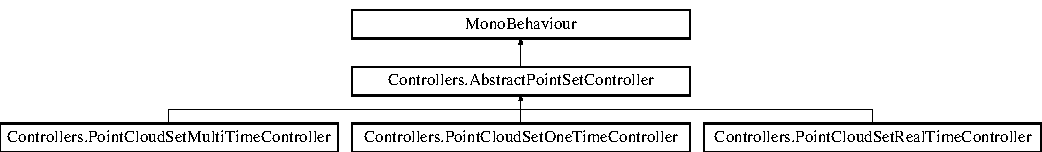
\includegraphics[height=2.043796cm]{class_controllers_1_1_abstract_point_set_controller}
\end{center}
\end{figure}
\subsection*{Public Member Functions}
\begin{DoxyCompactItemize}
\item 
\mbox{\Hypertarget{class_controllers_1_1_abstract_point_set_controller_a8bfeeed26c2cbc95ecfc3906fe39d932}\label{class_controllers_1_1_abstract_point_set_controller_a8bfeeed26c2cbc95ecfc3906fe39d932}} 
void {\bfseries Register\+Controller} (Mono\+Behaviour controller)
\item 
\mbox{\Hypertarget{class_controllers_1_1_abstract_point_set_controller_a10ea36265d82091cd92355ed64c2581c}\label{class_controllers_1_1_abstract_point_set_controller_a10ea36265d82091cd92355ed64c2581c}} 
void {\bfseries Update\+Bounding\+Box} (Mono\+Behaviour controller, \hyperlink{class_cloud_data_1_1_bounding_box}{Bounding\+Box} bounding\+Box)
\item 
\mbox{\Hypertarget{class_controllers_1_1_abstract_point_set_controller_aafa007a9fb523364254042ce85abbaf0}\label{class_controllers_1_1_abstract_point_set_controller_aafa007a9fb523364254042ce85abbaf0}} 
void {\bfseries Add\+Root\+Node} (\hyperlink{class_cloud_data_1_1_node}{Node} node)
\item 
\mbox{\Hypertarget{class_controllers_1_1_abstract_point_set_controller_a702c76d6d9a81a5a2878aafa428f8615}\label{class_controllers_1_1_abstract_point_set_controller_a702c76d6d9a81a5a2878aafa428f8615}} 
void {\bfseries On\+Application\+Quit} ()
\item 
\mbox{\Hypertarget{class_controllers_1_1_abstract_point_set_controller_a82db4e310b3d53990ca4ebffddd45bea}\label{class_controllers_1_1_abstract_point_set_controller_a82db4e310b3d53990ca4ebffddd45bea}} 
uint {\bfseries Get\+Point\+Count} ()
\end{DoxyCompactItemize}
\subsection*{Public Attributes}
\begin{DoxyCompactItemize}
\item 
\mbox{\Hypertarget{class_controllers_1_1_abstract_point_set_controller_a3c7db48c8fefd07e67df31986a265a30}\label{class_controllers_1_1_abstract_point_set_controller_a3c7db48c8fefd07e67df31986a265a30}} 
bool {\bfseries move\+Center\+To\+Transform\+Position} = true
\end{DoxyCompactItemize}
\subsection*{Protected Member Functions}
\begin{DoxyCompactItemize}
\item 
\mbox{\Hypertarget{class_controllers_1_1_abstract_point_set_controller_a8c7a3bc2173d6b23d8cd37b09c6cfe19}\label{class_controllers_1_1_abstract_point_set_controller_a8c7a3bc2173d6b23d8cd37b09c6cfe19}} 
abstract void {\bfseries Initialize} ()
\item 
\mbox{\Hypertarget{class_controllers_1_1_abstract_point_set_controller_a55485e0fbdd9f8154e140b2b79d0c787}\label{class_controllers_1_1_abstract_point_set_controller_a55485e0fbdd9f8154e140b2b79d0c787}} 
bool {\bfseries Check\+Ready} ()
\end{DoxyCompactItemize}
\subsection*{Properties}
\begin{DoxyCompactItemize}
\item 
\mbox{\Hypertarget{class_controllers_1_1_abstract_point_set_controller_ae05783b13871739392e1ce5fdb23ffbe}\label{class_controllers_1_1_abstract_point_set_controller_ae05783b13871739392e1ce5fdb23ffbe}} 
\hyperlink{interface_loading_1_1_abstract_renderer}{Abstract\+Renderer} {\bfseries Point\+Renderer}\hspace{0.3cm}{\ttfamily  \mbox{[}get, set\mbox{]}}
\end{DoxyCompactItemize}


The documentation for this class was generated from the following file\+:\begin{DoxyCompactItemize}
\item 
Controllers/Abstract\+Point\+Set\+Controller.\+cs\end{DoxyCompactItemize}

\hypertarget{interface_loading_1_1_abstract_renderer}{}\section{Loading.\+Abstract\+Renderer Interface Reference}
\label{interface_loading_1_1_abstract_renderer}\index{Loading.\+Abstract\+Renderer@{Loading.\+Abstract\+Renderer}}
Inheritance diagram for Loading.\+Abstract\+Renderer\+:\begin{figure}[H]
\begin{center}
\leavevmode
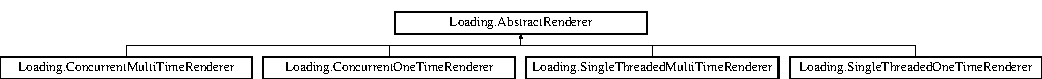
\includegraphics[height=1.060606cm]{interface_loading_1_1_abstract_renderer}
\end{center}
\end{figure}
\subsection*{Public Member Functions}
\begin{DoxyCompactItemize}
\item 
\mbox{\Hypertarget{interface_loading_1_1_abstract_renderer_a107159ee09c733ea8205fe47f8fac216}\label{interface_loading_1_1_abstract_renderer_a107159ee09c733ea8205fe47f8fac216}} 
void {\bfseries Add\+Root\+Node} (\hyperlink{class_cloud_data_1_1_node}{Node} root\+Node)
\item 
\mbox{\Hypertarget{interface_loading_1_1_abstract_renderer_ae6d660153792a10c7633f82be5010542}\label{interface_loading_1_1_abstract_renderer_ae6d660153792a10c7633f82be5010542}} 
int {\bfseries Get\+Root\+Node\+Count} ()
\item 
\mbox{\Hypertarget{interface_loading_1_1_abstract_renderer_a70e3721f67340976d72dd11cabdf4e4b}\label{interface_loading_1_1_abstract_renderer_a70e3721f67340976d72dd11cabdf4e4b}} 
bool {\bfseries Is\+Ready\+For\+Update} ()
\item 
\mbox{\Hypertarget{interface_loading_1_1_abstract_renderer_a0dbb8f2b8ad9ba83be923374bcdeda57}\label{interface_loading_1_1_abstract_renderer_a0dbb8f2b8ad9ba83be923374bcdeda57}} 
void {\bfseries Update\+Visible\+Nodes} ()
\item 
\mbox{\Hypertarget{interface_loading_1_1_abstract_renderer_ab78d3e23e2a4aea1f23337c661f11c54}\label{interface_loading_1_1_abstract_renderer_ab78d3e23e2a4aea1f23337c661f11c54}} 
void {\bfseries Update\+Game\+Objects} ()
\item 
\mbox{\Hypertarget{interface_loading_1_1_abstract_renderer_a005c3f95523559e7aece3f6bd88c6d0c}\label{interface_loading_1_1_abstract_renderer_a005c3f95523559e7aece3f6bd88c6d0c}} 
void {\bfseries Shut\+Down} ()
\item 
\mbox{\Hypertarget{interface_loading_1_1_abstract_renderer_a15b34dc6212c0d72c9e9837e0dd94391}\label{interface_loading_1_1_abstract_renderer_a15b34dc6212c0d72c9e9837e0dd94391}} 
uint {\bfseries Get\+Point\+Count} ()
\end{DoxyCompactItemize}


The documentation for this interface was generated from the following file\+:\begin{DoxyCompactItemize}
\item 
Loading/Abstract\+Renderer.\+cs\end{DoxyCompactItemize}

\hypertarget{class_cloud_data_1_1_bounding_box}{}\section{Cloud\+Data.\+Bounding\+Box Class Reference}
\label{class_cloud_data_1_1_bounding_box}\index{Cloud\+Data.\+Bounding\+Box@{Cloud\+Data.\+Bounding\+Box}}
\subsection*{Public Member Functions}
\begin{DoxyCompactItemize}
\item 
\mbox{\Hypertarget{class_cloud_data_1_1_bounding_box_a86e10f02158869d5ccc808e1826733da}\label{class_cloud_data_1_1_bounding_box_a86e10f02158869d5ccc808e1826733da}} 
{\bfseries Bounding\+Box} (double lx, double ly, double lz, double ux, double uy, double uz)
\item 
\mbox{\Hypertarget{class_cloud_data_1_1_bounding_box_a282c814d3b23ca4cd8597ed7e3ac2267}\label{class_cloud_data_1_1_bounding_box_a282c814d3b23ca4cd8597ed7e3ac2267}} 
{\bfseries Bounding\+Box} (\hyperlink{class_cloud_data_1_1_vector3d}{Vector3d} min, \hyperlink{class_cloud_data_1_1_vector3d}{Vector3d} max)
\item 
\mbox{\Hypertarget{class_cloud_data_1_1_bounding_box_a6e915fefab3d9283d229c0e2b1299c74}\label{class_cloud_data_1_1_bounding_box_a6e915fefab3d9283d229c0e2b1299c74}} 
void {\bfseries Init} ()
\item 
\mbox{\Hypertarget{class_cloud_data_1_1_bounding_box_afdab2adfb0afb14d7b9f92f552d7d768}\label{class_cloud_data_1_1_bounding_box_afdab2adfb0afb14d7b9f92f552d7d768}} 
void {\bfseries Switch\+YZ} ()
\item 
\mbox{\Hypertarget{class_cloud_data_1_1_bounding_box_a00101639964ec22073a0f5b40e65d051}\label{class_cloud_data_1_1_bounding_box_a00101639964ec22073a0f5b40e65d051}} 
void {\bfseries Move\+To\+Origin} ()
\item 
\mbox{\Hypertarget{class_cloud_data_1_1_bounding_box_a46071c421dcd1259018cd1132a70eeb6}\label{class_cloud_data_1_1_bounding_box_a46071c421dcd1259018cd1132a70eeb6}} 
void {\bfseries Move\+Along} (\hyperlink{class_cloud_data_1_1_vector3d}{Vector3d} vector)
\item 
\mbox{\Hypertarget{class_cloud_data_1_1_bounding_box_a080446f806f02227b9b45da11f8d02d6}\label{class_cloud_data_1_1_bounding_box_a080446f806f02227b9b45da11f8d02d6}} 
double {\bfseries Radius} ()
\item 
\mbox{\Hypertarget{class_cloud_data_1_1_bounding_box_adca189994b00ae2faf2293b8ef46f9cd}\label{class_cloud_data_1_1_bounding_box_adca189994b00ae2faf2293b8ef46f9cd}} 
\hyperlink{class_cloud_data_1_1_vector3d}{Vector3d} {\bfseries Size} ()
\item 
\mbox{\Hypertarget{class_cloud_data_1_1_bounding_box_aa477d033f2fb789db62444d388508767}\label{class_cloud_data_1_1_bounding_box_aa477d033f2fb789db62444d388508767}} 
\hyperlink{class_cloud_data_1_1_vector3d}{Vector3d} {\bfseries Min} ()
\item 
\mbox{\Hypertarget{class_cloud_data_1_1_bounding_box_a9fed7b597fc4bcded540dbb8484c9327}\label{class_cloud_data_1_1_bounding_box_a9fed7b597fc4bcded540dbb8484c9327}} 
\hyperlink{class_cloud_data_1_1_vector3d}{Vector3d} {\bfseries Max} ()
\item 
\mbox{\Hypertarget{class_cloud_data_1_1_bounding_box_ad645b50a22a9d532bc64012513b5bae7}\label{class_cloud_data_1_1_bounding_box_ad645b50a22a9d532bc64012513b5bae7}} 
\hyperlink{class_cloud_data_1_1_vector3d}{Vector3d} {\bfseries Center} ()
\item 
\mbox{\Hypertarget{class_cloud_data_1_1_bounding_box_af805e886dc37ca582682256e3f7c282b}\label{class_cloud_data_1_1_bounding_box_af805e886dc37ca582682256e3f7c282b}} 
Bounds {\bfseries Get\+Bounds\+Object} ()
\item 
\mbox{\Hypertarget{class_cloud_data_1_1_bounding_box_ad38a3857856aa40d986d7c692762e05e}\label{class_cloud_data_1_1_bounding_box_ad38a3857856aa40d986d7c692762e05e}} 
override string {\bfseries To\+String} ()
\end{DoxyCompactItemize}
\subsection*{Public Attributes}
\begin{DoxyCompactItemize}
\item 
\mbox{\Hypertarget{class_cloud_data_1_1_bounding_box_afccc6119b7307c1a4847797155455939}\label{class_cloud_data_1_1_bounding_box_afccc6119b7307c1a4847797155455939}} 
double {\bfseries lx}
\item 
\mbox{\Hypertarget{class_cloud_data_1_1_bounding_box_a338a758672564c211249b8eb2388b2b2}\label{class_cloud_data_1_1_bounding_box_a338a758672564c211249b8eb2388b2b2}} 
double {\bfseries ly}
\item 
\mbox{\Hypertarget{class_cloud_data_1_1_bounding_box_a9ce1d3eca3a29640c7c8591802e1c795}\label{class_cloud_data_1_1_bounding_box_a9ce1d3eca3a29640c7c8591802e1c795}} 
double {\bfseries lz}
\item 
\mbox{\Hypertarget{class_cloud_data_1_1_bounding_box_a5eb9a578bd7ed40abc6f7103ae47b3fb}\label{class_cloud_data_1_1_bounding_box_a5eb9a578bd7ed40abc6f7103ae47b3fb}} 
double {\bfseries ux}
\item 
\mbox{\Hypertarget{class_cloud_data_1_1_bounding_box_ae25969523e322b6bd1f181476cf2243c}\label{class_cloud_data_1_1_bounding_box_ae25969523e322b6bd1f181476cf2243c}} 
double {\bfseries uy}
\item 
\mbox{\Hypertarget{class_cloud_data_1_1_bounding_box_a35362a75e3fe95e287464c370f1b6f99}\label{class_cloud_data_1_1_bounding_box_a35362a75e3fe95e287464c370f1b6f99}} 
double {\bfseries uz}
\end{DoxyCompactItemize}
\subsection*{Properties}
\begin{DoxyCompactItemize}
\item 
\mbox{\Hypertarget{class_cloud_data_1_1_bounding_box_a5b1c5fb7f1aa969b229ddc3b90eebd4f}\label{class_cloud_data_1_1_bounding_box_a5b1c5fb7f1aa969b229ddc3b90eebd4f}} 
double {\bfseries Lx}\hspace{0.3cm}{\ttfamily  \mbox{[}get, set\mbox{]}}
\item 
\mbox{\Hypertarget{class_cloud_data_1_1_bounding_box_a8c6bc25680269352356dd8dfbdba6d56}\label{class_cloud_data_1_1_bounding_box_a8c6bc25680269352356dd8dfbdba6d56}} 
double {\bfseries Ly}\hspace{0.3cm}{\ttfamily  \mbox{[}get, set\mbox{]}}
\item 
\mbox{\Hypertarget{class_cloud_data_1_1_bounding_box_a419d5665cf475e9f21747d651162e7e4}\label{class_cloud_data_1_1_bounding_box_a419d5665cf475e9f21747d651162e7e4}} 
double {\bfseries Lz}\hspace{0.3cm}{\ttfamily  \mbox{[}get, set\mbox{]}}
\item 
\mbox{\Hypertarget{class_cloud_data_1_1_bounding_box_aebeb49a340501e573d02d828c4457560}\label{class_cloud_data_1_1_bounding_box_aebeb49a340501e573d02d828c4457560}} 
double {\bfseries Ux}\hspace{0.3cm}{\ttfamily  \mbox{[}get, set\mbox{]}}
\item 
\mbox{\Hypertarget{class_cloud_data_1_1_bounding_box_a6949e58d591077d9989177883bbd46ea}\label{class_cloud_data_1_1_bounding_box_a6949e58d591077d9989177883bbd46ea}} 
double {\bfseries Uy}\hspace{0.3cm}{\ttfamily  \mbox{[}get, set\mbox{]}}
\item 
\mbox{\Hypertarget{class_cloud_data_1_1_bounding_box_a5d242c32897b18aa60d6ce3659278ee6}\label{class_cloud_data_1_1_bounding_box_a5d242c32897b18aa60d6ce3659278ee6}} 
double {\bfseries Uz}\hspace{0.3cm}{\ttfamily  \mbox{[}get, set\mbox{]}}
\end{DoxyCompactItemize}


The documentation for this class was generated from the following file\+:\begin{DoxyCompactItemize}
\item 
Cloud\+Data/Bounding\+Box.\+cs\end{DoxyCompactItemize}

\hypertarget{class_controllers_1_1_camera_controller}{}\section{Controllers.\+Camera\+Controller Class Reference}
\label{class_controllers_1_1_camera_controller}\index{Controllers.\+Camera\+Controller@{Controllers.\+Camera\+Controller}}
Inheritance diagram for Controllers.\+Camera\+Controller\+:\begin{figure}[H]
\begin{center}
\leavevmode
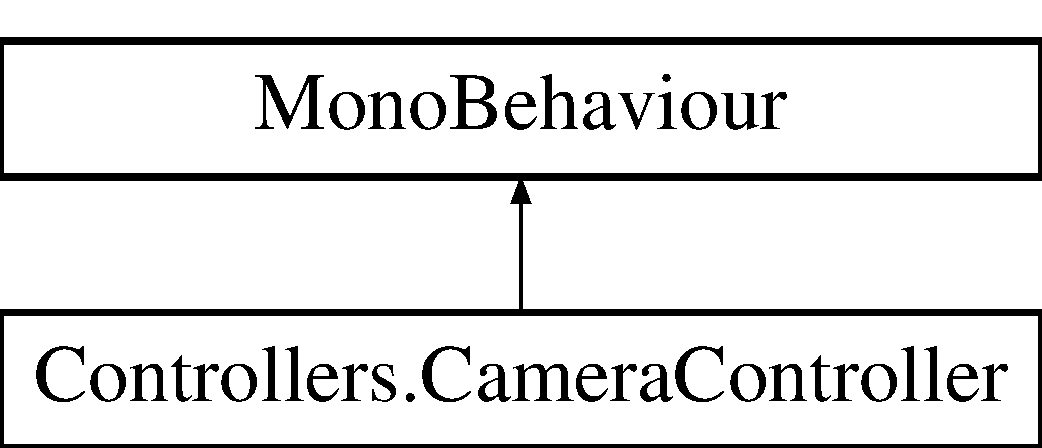
\includegraphics[height=2.000000cm]{class_controllers_1_1_camera_controller}
\end{center}
\end{figure}


The documentation for this class was generated from the following file\+:\begin{DoxyCompactItemize}
\item 
Controllers/Camera\+Controller.\+cs\end{DoxyCompactItemize}

\hypertarget{class_loading_1_1_cloud_loader}{}\section{Loading.\+Cloud\+Loader Class Reference}
\label{class_loading_1_1_cloud_loader}\index{Loading.\+Cloud\+Loader@{Loading.\+Cloud\+Loader}}
\subsection*{Static Public Member Functions}
\begin{DoxyCompactItemize}
\item 
\mbox{\Hypertarget{class_loading_1_1_cloud_loader_a234660c32f4fa182426e11b597149821}\label{class_loading_1_1_cloud_loader_a234660c32f4fa182426e11b597149821}} 
static \hyperlink{class_cloud_data_1_1_point_cloud_meta_data}{Point\+Cloud\+Meta\+Data} {\bfseries Load\+Meta\+Data} (string cloud\+Path, bool move\+To\+Origin=false)
\item 
\mbox{\Hypertarget{class_loading_1_1_cloud_loader_a4a3de7574dec7b35d70ff2a51c09353f}\label{class_loading_1_1_cloud_loader_a4a3de7574dec7b35d70ff2a51c09353f}} 
static \hyperlink{class_cloud_data_1_1_node}{Node} {\bfseries Load\+Point\+Cloud} (string cloud\+Path, \hyperlink{class_cloud_data_1_1_point_cloud_meta_data}{Point\+Cloud\+Meta\+Data} meta\+Data)
\item 
\mbox{\Hypertarget{class_loading_1_1_cloud_loader_a13e35349e28c5091565880d77bc3423a}\label{class_loading_1_1_cloud_loader_a13e35349e28c5091565880d77bc3423a}} 
static \hyperlink{class_cloud_data_1_1_node}{Node} {\bfseries Load\+Hierarchy\+Only} (\hyperlink{class_cloud_data_1_1_point_cloud_meta_data}{Point\+Cloud\+Meta\+Data} meta\+Data)
\item 
\mbox{\Hypertarget{class_loading_1_1_cloud_loader_a623c96ee2eee44b30b86fea2661fcbd8}\label{class_loading_1_1_cloud_loader_a623c96ee2eee44b30b86fea2661fcbd8}} 
static void {\bfseries Load\+Points\+For\+Node} (\hyperlink{class_cloud_data_1_1_node}{Node} node)
\end{DoxyCompactItemize}


The documentation for this class was generated from the following file\+:\begin{DoxyCompactItemize}
\item 
Loading/Cloud\+Loader.\+cs\end{DoxyCompactItemize}

\hypertarget{class_controllers_1_1_clouds_from_directory_loader}{}\section{Controllers.\+Clouds\+From\+Directory\+Loader Class Reference}
\label{class_controllers_1_1_clouds_from_directory_loader}\index{Controllers.\+Clouds\+From\+Directory\+Loader@{Controllers.\+Clouds\+From\+Directory\+Loader}}
Inheritance diagram for Controllers.\+Clouds\+From\+Directory\+Loader\+:\begin{figure}[H]
\begin{center}
\leavevmode
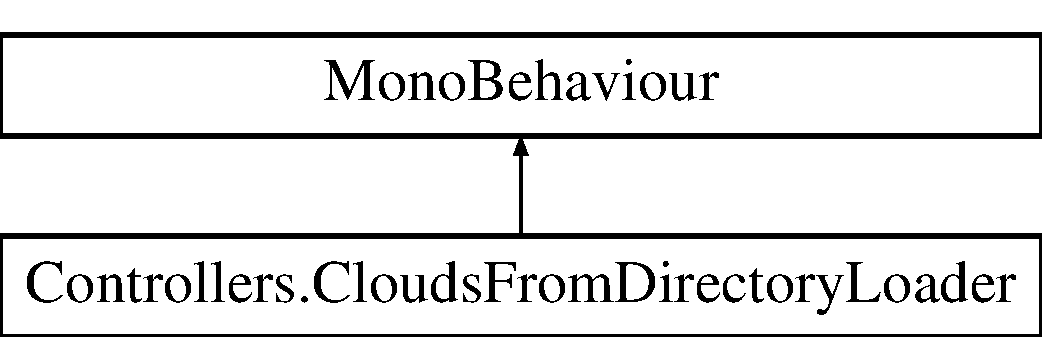
\includegraphics[height=2.000000cm]{class_controllers_1_1_clouds_from_directory_loader}
\end{center}
\end{figure}
\subsection*{Public Attributes}
\begin{DoxyCompactItemize}
\item 
\mbox{\Hypertarget{class_controllers_1_1_clouds_from_directory_loader_a51d5ebe509e8dd85161489c163bebe42}\label{class_controllers_1_1_clouds_from_directory_loader_a51d5ebe509e8dd85161489c163bebe42}} 
string {\bfseries path}
\item 
\mbox{\Hypertarget{class_controllers_1_1_clouds_from_directory_loader_ae8b5d29d07e3e737498199a90c43e8f6}\label{class_controllers_1_1_clouds_from_directory_loader_ae8b5d29d07e3e737498199a90c43e8f6}} 
\hyperlink{class_controllers_1_1_abstract_point_set_controller}{Abstract\+Point\+Set\+Controller} {\bfseries pointset}
\end{DoxyCompactItemize}


The documentation for this class was generated from the following file\+:\begin{DoxyCompactItemize}
\item 
Controllers/Clouds\+From\+Directory\+Loader.\+cs\end{DoxyCompactItemize}

\hypertarget{class_loading_1_1_concurrent_multi_time_renderer}{}\section{Loading.\+Concurrent\+Multi\+Time\+Renderer Class Reference}
\label{class_loading_1_1_concurrent_multi_time_renderer}\index{Loading.\+Concurrent\+Multi\+Time\+Renderer@{Loading.\+Concurrent\+Multi\+Time\+Renderer}}
Inheritance diagram for Loading.\+Concurrent\+Multi\+Time\+Renderer\+:\begin{figure}[H]
\begin{center}
\leavevmode
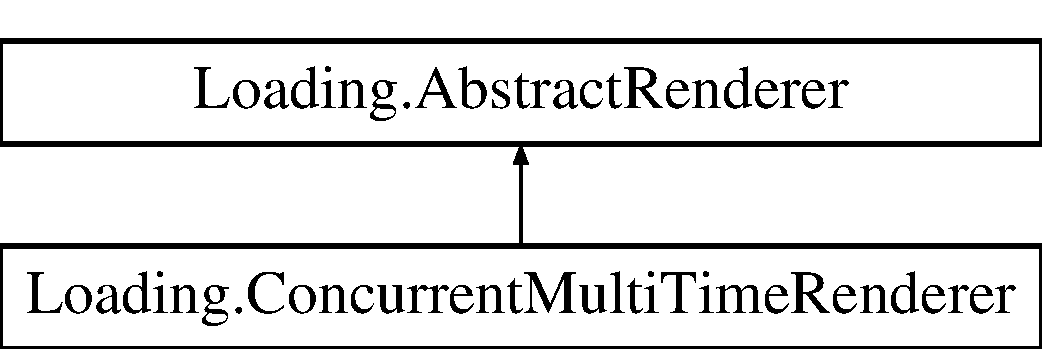
\includegraphics[height=2.000000cm]{class_loading_1_1_concurrent_multi_time_renderer}
\end{center}
\end{figure}
\subsection*{Public Member Functions}
\begin{DoxyCompactItemize}
\item 
\mbox{\Hypertarget{class_loading_1_1_concurrent_multi_time_renderer_ad368df666c756e4541af205b930640bf}\label{class_loading_1_1_concurrent_multi_time_renderer_ad368df666c756e4541af205b930640bf}} 
{\bfseries Concurrent\+Multi\+Time\+Renderer} (int min\+Node\+Size, uint point\+Budget, uint nodes\+Per\+Frame, Camera camera, \hyperlink{class_object_creation_1_1_mesh_configuration}{Mesh\+Configuration} config, uint cache\+Size\+In\+Points)
\item 
\mbox{\Hypertarget{class_loading_1_1_concurrent_multi_time_renderer_a92ef20bfb5177d3e1afa9ee3327f3449}\label{class_loading_1_1_concurrent_multi_time_renderer_a92ef20bfb5177d3e1afa9ee3327f3449}} 
void {\bfseries Add\+Root\+Node} (\hyperlink{class_cloud_data_1_1_node}{Node} root\+Node)
\item 
\mbox{\Hypertarget{class_loading_1_1_concurrent_multi_time_renderer_adceaa06267aefc6cca72ff9f44f354d8}\label{class_loading_1_1_concurrent_multi_time_renderer_adceaa06267aefc6cca72ff9f44f354d8}} 
int {\bfseries Get\+Root\+Node\+Count} ()
\item 
\mbox{\Hypertarget{class_loading_1_1_concurrent_multi_time_renderer_a161bda4ed67d267fec6ba5ccce44d5b9}\label{class_loading_1_1_concurrent_multi_time_renderer_a161bda4ed67d267fec6ba5ccce44d5b9}} 
bool {\bfseries Is\+Ready\+For\+Update} ()
\item 
\mbox{\Hypertarget{class_loading_1_1_concurrent_multi_time_renderer_abe0bd3b605af54b60630d9a558dda7b2}\label{class_loading_1_1_concurrent_multi_time_renderer_abe0bd3b605af54b60630d9a558dda7b2}} 
void {\bfseries Update\+Visible\+Nodes} ()
\item 
\mbox{\Hypertarget{class_loading_1_1_concurrent_multi_time_renderer_a147eb4990903757e4fde6968f0ef50dc}\label{class_loading_1_1_concurrent_multi_time_renderer_a147eb4990903757e4fde6968f0ef50dc}} 
void {\bfseries Update\+Game\+Objects} ()
\item 
\mbox{\Hypertarget{class_loading_1_1_concurrent_multi_time_renderer_a5d4c4db0c0d0fd7ae91a5129e89d12f3}\label{class_loading_1_1_concurrent_multi_time_renderer_a5d4c4db0c0d0fd7ae91a5129e89d12f3}} 
void {\bfseries Shut\+Down} ()
\item 
\mbox{\Hypertarget{class_loading_1_1_concurrent_multi_time_renderer_a1f3e936364cb90d633aa1ca97f2e3981}\label{class_loading_1_1_concurrent_multi_time_renderer_a1f3e936364cb90d633aa1ca97f2e3981}} 
uint {\bfseries Get\+Point\+Count} ()
\end{DoxyCompactItemize}


The documentation for this class was generated from the following file\+:\begin{DoxyCompactItemize}
\item 
Loading/Concurrent\+Multi\+Time\+Renderer.\+cs\end{DoxyCompactItemize}

\hypertarget{class_loading_1_1_concurrent_one_time_renderer}{}\section{Loading.\+Concurrent\+One\+Time\+Renderer Class Reference}
\label{class_loading_1_1_concurrent_one_time_renderer}\index{Loading.\+Concurrent\+One\+Time\+Renderer@{Loading.\+Concurrent\+One\+Time\+Renderer}}
Inheritance diagram for Loading.\+Concurrent\+One\+Time\+Renderer\+:\begin{figure}[H]
\begin{center}
\leavevmode
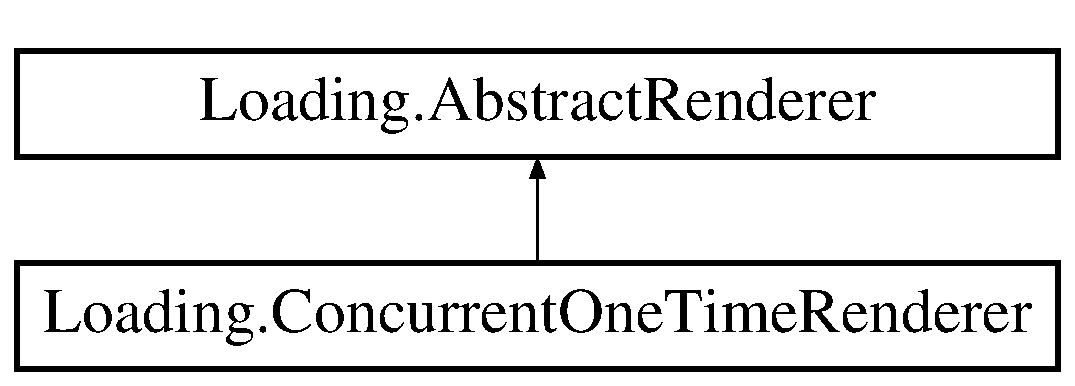
\includegraphics[height=2.000000cm]{class_loading_1_1_concurrent_one_time_renderer}
\end{center}
\end{figure}
\subsection*{Public Member Functions}
\begin{DoxyCompactItemize}
\item 
\mbox{\Hypertarget{class_loading_1_1_concurrent_one_time_renderer_ad51208fab2b19f9641b0143d9138101f}\label{class_loading_1_1_concurrent_one_time_renderer_ad51208fab2b19f9641b0143d9138101f}} 
{\bfseries Concurrent\+One\+Time\+Renderer} (int min\+Node\+Size, uint point\+Budget, Camera camera, \hyperlink{class_object_creation_1_1_mesh_configuration}{Mesh\+Configuration} config)
\item 
\mbox{\Hypertarget{class_loading_1_1_concurrent_one_time_renderer_a60a4f399a0640015374a5c31e7ea20ce}\label{class_loading_1_1_concurrent_one_time_renderer_a60a4f399a0640015374a5c31e7ea20ce}} 
void {\bfseries Add\+Root\+Node} (\hyperlink{class_cloud_data_1_1_node}{Node} root\+Node)
\item 
\mbox{\Hypertarget{class_loading_1_1_concurrent_one_time_renderer_afaf15e37da51bde9eb28474b77e1e2c6}\label{class_loading_1_1_concurrent_one_time_renderer_afaf15e37da51bde9eb28474b77e1e2c6}} 
int {\bfseries Get\+Root\+Node\+Count} ()
\item 
\mbox{\Hypertarget{class_loading_1_1_concurrent_one_time_renderer_a8484b61d6d8f790acb3760835c309d39}\label{class_loading_1_1_concurrent_one_time_renderer_a8484b61d6d8f790acb3760835c309d39}} 
bool {\bfseries Is\+Ready\+For\+Update} ()
\item 
\mbox{\Hypertarget{class_loading_1_1_concurrent_one_time_renderer_a86dccdf9d91c01272901bc8f6c106939}\label{class_loading_1_1_concurrent_one_time_renderer_a86dccdf9d91c01272901bc8f6c106939}} 
void {\bfseries Update\+Visible\+Nodes} ()
\item 
\mbox{\Hypertarget{class_loading_1_1_concurrent_one_time_renderer_a4b6e2f1b866ba77102e3db297cc53d0c}\label{class_loading_1_1_concurrent_one_time_renderer_a4b6e2f1b866ba77102e3db297cc53d0c}} 
void {\bfseries Update\+Game\+Objects} ()
\item 
\mbox{\Hypertarget{class_loading_1_1_concurrent_one_time_renderer_a5174a5558f8fb4221cf0b29264108d17}\label{class_loading_1_1_concurrent_one_time_renderer_a5174a5558f8fb4221cf0b29264108d17}} 
void {\bfseries Shut\+Down} ()
\item 
\mbox{\Hypertarget{class_loading_1_1_concurrent_one_time_renderer_a9aa238b23680098aab7a36f1dd9363d5}\label{class_loading_1_1_concurrent_one_time_renderer_a9aa238b23680098aab7a36f1dd9363d5}} 
uint {\bfseries Get\+Point\+Count} ()
\end{DoxyCompactItemize}


The documentation for this class was generated from the following file\+:\begin{DoxyCompactItemize}
\item 
Loading/Concurrent\+One\+Time\+Renderer.\+cs\end{DoxyCompactItemize}

\hypertarget{class_data_structures_1_1_dictionary_priority_queue}{}\section{Data\+Structures.\+Dictionary\+Priority\+Queue$<$ I, T $>$ Class Template Reference}
\label{class_data_structures_1_1_dictionary_priority_queue}\index{Data\+Structures.\+Dictionary\+Priority\+Queue$<$ I, T $>$@{Data\+Structures.\+Dictionary\+Priority\+Queue$<$ I, T $>$}}
Inheritance diagram for Data\+Structures.\+Dictionary\+Priority\+Queue$<$ I, T $>$\+:\begin{figure}[H]
\begin{center}
\leavevmode
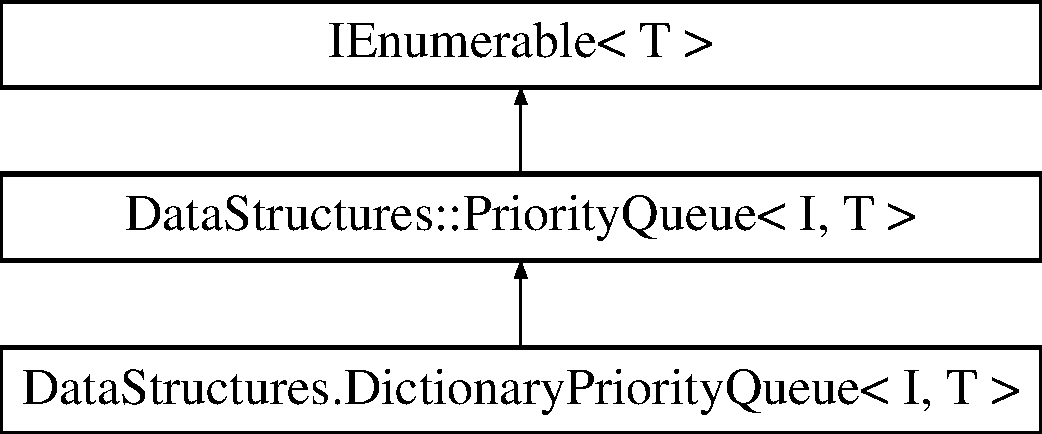
\includegraphics[height=3.000000cm]{class_data_structures_1_1_dictionary_priority_queue}
\end{center}
\end{figure}
\subsection*{Public Member Functions}
\begin{DoxyCompactItemize}
\item 
\mbox{\Hypertarget{class_data_structures_1_1_dictionary_priority_queue_ae1a318c96ce4c1883ddacd54e8f6ba1b}\label{class_data_structures_1_1_dictionary_priority_queue_ae1a318c96ce4c1883ddacd54e8f6ba1b}} 
override void {\bfseries Enqueue} (T element, I priority)
\item 
\mbox{\Hypertarget{class_data_structures_1_1_dictionary_priority_queue_ad7c339039d268e493bcf409f47132bac}\label{class_data_structures_1_1_dictionary_priority_queue_ad7c339039d268e493bcf409f47132bac}} 
override T {\bfseries Dequeue} ()
\item 
\mbox{\Hypertarget{class_data_structures_1_1_dictionary_priority_queue_a6e14cf527b211617ad0ca35f1ca858df}\label{class_data_structures_1_1_dictionary_priority_queue_a6e14cf527b211617ad0ca35f1ca858df}} 
override T {\bfseries Dequeue} (out I priority)
\item 
\mbox{\Hypertarget{class_data_structures_1_1_dictionary_priority_queue_a9078255b0ea0c46dab3a733cb3873def}\label{class_data_structures_1_1_dictionary_priority_queue_a9078255b0ea0c46dab3a733cb3873def}} 
override I {\bfseries Max\+Priority} ()
\item 
\mbox{\Hypertarget{class_data_structures_1_1_dictionary_priority_queue_a7a3d883ab0c5c4996283f09f6815bd39}\label{class_data_structures_1_1_dictionary_priority_queue_a7a3d883ab0c5c4996283f09f6815bd39}} 
override T {\bfseries Peek} ()
\item 
\mbox{\Hypertarget{class_data_structures_1_1_dictionary_priority_queue_abc1dc4375ee6ce2763ff97ead9ad3e32}\label{class_data_structures_1_1_dictionary_priority_queue_abc1dc4375ee6ce2763ff97ead9ad3e32}} 
override void {\bfseries Clear} ()
\item 
\mbox{\Hypertarget{class_data_structures_1_1_dictionary_priority_queue_a53d92460413448967da3a78749b498fa}\label{class_data_structures_1_1_dictionary_priority_queue_a53d92460413448967da3a78749b498fa}} 
override bool {\bfseries Is\+Empty} ()
\item 
\mbox{\Hypertarget{class_data_structures_1_1_dictionary_priority_queue_a295d48e96f81382cf6c4a5da209f87ec}\label{class_data_structures_1_1_dictionary_priority_queue_a295d48e96f81382cf6c4a5da209f87ec}} 
override I\+Enumerator$<$ T $>$ {\bfseries Get\+Enumerator} ()
\item 
\mbox{\Hypertarget{class_data_structures_1_1_dictionary_priority_queue_aa53f5407a243ffd3e34b1c592fad1519}\label{class_data_structures_1_1_dictionary_priority_queue_aa53f5407a243ffd3e34b1c592fad1519}} 
override void {\bfseries Remove} (T element, I priority)
\item 
\mbox{\Hypertarget{class_data_structures_1_1_dictionary_priority_queue_addcd9304fb91872988246d6685e48d84}\label{class_data_structures_1_1_dictionary_priority_queue_addcd9304fb91872988246d6685e48d84}} 
override void {\bfseries Remove} (T element)
\end{DoxyCompactItemize}
\subsection*{Properties}
\begin{DoxyCompactItemize}
\item 
\mbox{\Hypertarget{class_data_structures_1_1_dictionary_priority_queue_a1bd59231ffc3caf8826a8a10bb4fbf03}\label{class_data_structures_1_1_dictionary_priority_queue_a1bd59231ffc3caf8826a8a10bb4fbf03}} 
override int {\bfseries Count}\hspace{0.3cm}{\ttfamily  \mbox{[}get\mbox{]}}
\end{DoxyCompactItemize}


The documentation for this class was generated from the following file\+:\begin{DoxyCompactItemize}
\item 
Data\+Structures/Dictionary\+Priority\+Queue.\+cs\end{DoxyCompactItemize}

\hypertarget{class_controllers_1_1_dynamic_loader_controller}{}\section{Controllers.\+Dynamic\+Loader\+Controller Class Reference}
\label{class_controllers_1_1_dynamic_loader_controller}\index{Controllers.\+Dynamic\+Loader\+Controller@{Controllers.\+Dynamic\+Loader\+Controller}}
Inheritance diagram for Controllers.\+Dynamic\+Loader\+Controller\+:\begin{figure}[H]
\begin{center}
\leavevmode
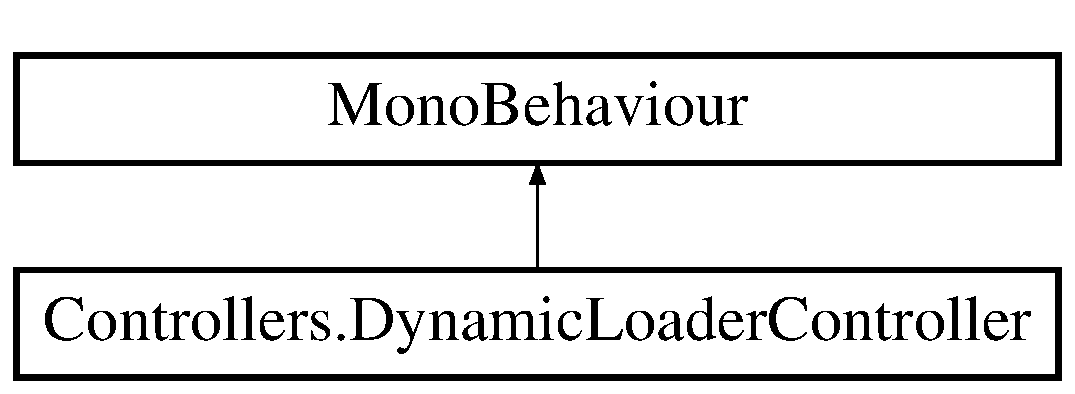
\includegraphics[height=2.000000cm]{class_controllers_1_1_dynamic_loader_controller}
\end{center}
\end{figure}
\subsection*{Public Attributes}
\begin{DoxyCompactItemize}
\item 
\mbox{\Hypertarget{class_controllers_1_1_dynamic_loader_controller_afe909bbcb95428500b939c911a21ea4a}\label{class_controllers_1_1_dynamic_loader_controller_afe909bbcb95428500b939c911a21ea4a}} 
string {\bfseries cloud\+Path}
\item 
\mbox{\Hypertarget{class_controllers_1_1_dynamic_loader_controller_a521c29ad1518e963c692df3e462fd168}\label{class_controllers_1_1_dynamic_loader_controller_a521c29ad1518e963c692df3e462fd168}} 
\hyperlink{class_controllers_1_1_abstract_point_set_controller}{Abstract\+Point\+Set\+Controller} {\bfseries set\+Controller}
\end{DoxyCompactItemize}


The documentation for this class was generated from the following file\+:\begin{DoxyCompactItemize}
\item 
Controllers/Dynamic\+Loader\+Controller.\+cs\end{DoxyCompactItemize}

\hypertarget{class_controllers_1_1_f_p_s_output_controller}{}\section{Controllers.\+F\+P\+S\+Output\+Controller Class Reference}
\label{class_controllers_1_1_f_p_s_output_controller}\index{Controllers.\+F\+P\+S\+Output\+Controller@{Controllers.\+F\+P\+S\+Output\+Controller}}
Inheritance diagram for Controllers.\+F\+P\+S\+Output\+Controller\+:\begin{figure}[H]
\begin{center}
\leavevmode
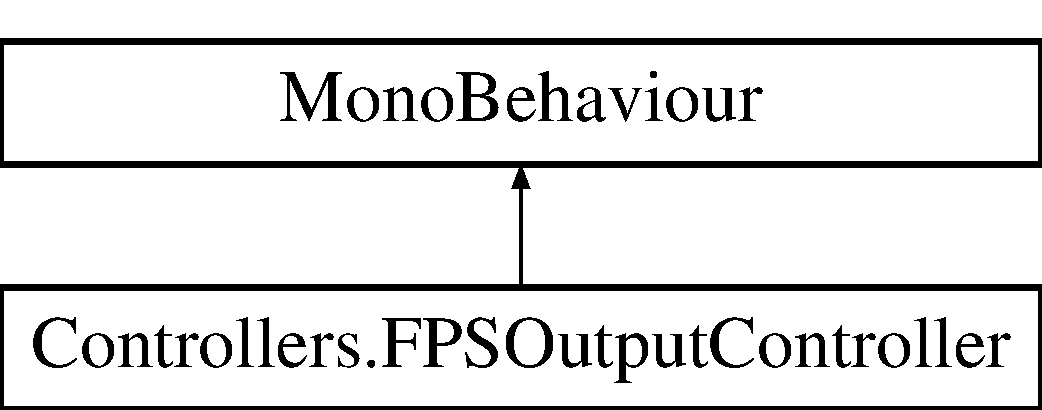
\includegraphics[height=2.000000cm]{class_controllers_1_1_f_p_s_output_controller}
\end{center}
\end{figure}
\subsection*{Static Public Member Functions}
\begin{DoxyCompactItemize}
\item 
\mbox{\Hypertarget{class_controllers_1_1_f_p_s_output_controller_a628a1c694c212ad4148aef85aa6a5634}\label{class_controllers_1_1_f_p_s_output_controller_a628a1c694c212ad4148aef85aa6a5634}} 
static void {\bfseries Note\+F\+PS} (bool flush)
\end{DoxyCompactItemize}
\subsection*{Public Attributes}
\begin{DoxyCompactItemize}
\item 
\mbox{\Hypertarget{class_controllers_1_1_f_p_s_output_controller_ad70bd399d1f66b55969d7bd731647503}\label{class_controllers_1_1_f_p_s_output_controller_ad70bd399d1f66b55969d7bd731647503}} 
float {\bfseries output\+Interval} = 1
\item 
\mbox{\Hypertarget{class_controllers_1_1_f_p_s_output_controller_ae5e3b6dfd49f7fa25df8309a98980865}\label{class_controllers_1_1_f_p_s_output_controller_ae5e3b6dfd49f7fa25df8309a98980865}} 
\hyperlink{class_controllers_1_1_abstract_point_set_controller}{Abstract\+Point\+Set\+Controller} {\bfseries pointset} = null
\end{DoxyCompactItemize}


The documentation for this class was generated from the following file\+:\begin{DoxyCompactItemize}
\item 
Controllers/F\+P\+S\+Output\+Controller.\+cs\end{DoxyCompactItemize}

\hypertarget{class_loading_1_1_game_object_l_r_u_cache}{}\section{Loading.\+Game\+Object\+L\+R\+U\+Cache Class Reference}
\label{class_loading_1_1_game_object_l_r_u_cache}\index{Loading.\+Game\+Object\+L\+R\+U\+Cache@{Loading.\+Game\+Object\+L\+R\+U\+Cache}}
\subsection*{Public Member Functions}
\begin{DoxyCompactItemize}
\item 
\mbox{\Hypertarget{class_loading_1_1_game_object_l_r_u_cache_a5b9fce889473f38bab25a33d1679801f}\label{class_loading_1_1_game_object_l_r_u_cache_a5b9fce889473f38bab25a33d1679801f}} 
void {\bfseries Insert} (\hyperlink{class_cloud_data_1_1_node}{Node} node)
\item 
\mbox{\Hypertarget{class_loading_1_1_game_object_l_r_u_cache_ac6cd29fdf26f70d74c205b02f150367d}\label{class_loading_1_1_game_object_l_r_u_cache_ac6cd29fdf26f70d74c205b02f150367d}} 
void {\bfseries Withdraw} (\hyperlink{class_cloud_data_1_1_node}{Node} node)
\end{DoxyCompactItemize}
\subsection*{Static Public Member Functions}
\begin{DoxyCompactItemize}
\item 
\mbox{\Hypertarget{class_loading_1_1_game_object_l_r_u_cache_a2e91558444a80a8240d03218fbc33e63}\label{class_loading_1_1_game_object_l_r_u_cache_a2e91558444a80a8240d03218fbc33e63}} 
static \hyperlink{class_loading_1_1_game_object_l_r_u_cache}{Game\+Object\+L\+R\+U\+Cache} {\bfseries Cache\+From\+Byte\+Size} (uint byte\+Size, \hyperlink{class_object_creation_1_1_mesh_configuration}{Mesh\+Configuration} config)
\item 
\mbox{\Hypertarget{class_loading_1_1_game_object_l_r_u_cache_af42e0f3663aaea70de0e054c2111ffcf}\label{class_loading_1_1_game_object_l_r_u_cache_af42e0f3663aaea70de0e054c2111ffcf}} 
static \hyperlink{class_loading_1_1_game_object_l_r_u_cache}{Game\+Object\+L\+R\+U\+Cache} {\bfseries Cache\+From\+Point\+Count} (uint point\+Count, \hyperlink{class_object_creation_1_1_mesh_configuration}{Mesh\+Configuration} config)
\end{DoxyCompactItemize}


The documentation for this class was generated from the following file\+:\begin{DoxyCompactItemize}
\item 
Loading/Game\+Object\+L\+R\+U\+Cache.\+cs\end{DoxyCompactItemize}

\hypertarget{class_object_creation_1_1_geo_quad_mesh_configuration}{}\section{Object\+Creation.\+Geo\+Quad\+Mesh\+Configuration Class Reference}
\label{class_object_creation_1_1_geo_quad_mesh_configuration}\index{Object\+Creation.\+Geo\+Quad\+Mesh\+Configuration@{Object\+Creation.\+Geo\+Quad\+Mesh\+Configuration}}
Inheritance diagram for Object\+Creation.\+Geo\+Quad\+Mesh\+Configuration\+:\begin{figure}[H]
\begin{center}
\leavevmode
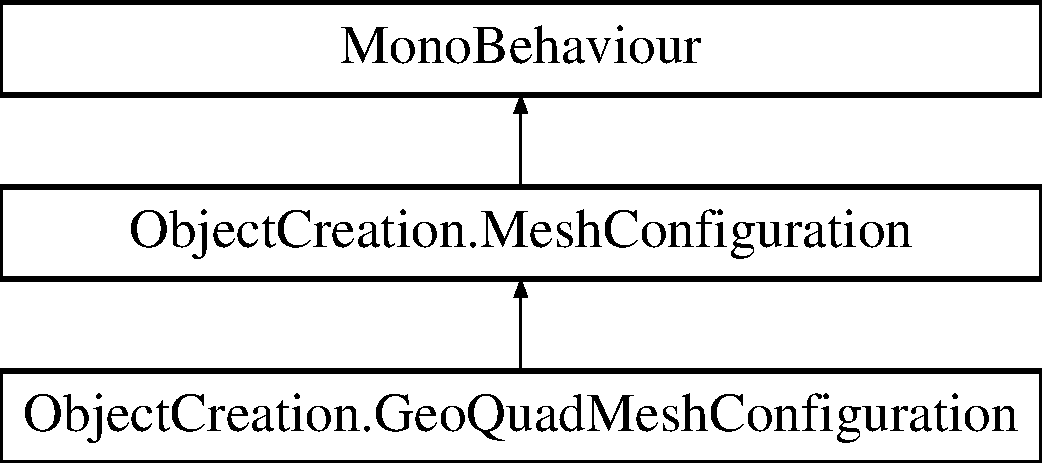
\includegraphics[height=3.000000cm]{class_object_creation_1_1_geo_quad_mesh_configuration}
\end{center}
\end{figure}
\subsection*{Public Member Functions}
\begin{DoxyCompactItemize}
\item 
\mbox{\Hypertarget{class_object_creation_1_1_geo_quad_mesh_configuration_aa3be631b1edfd389b2b4c26d434336e6}\label{class_object_creation_1_1_geo_quad_mesh_configuration_aa3be631b1edfd389b2b4c26d434336e6}} 
void {\bfseries Start} ()
\item 
\mbox{\Hypertarget{class_object_creation_1_1_geo_quad_mesh_configuration_ae18fc554f81e3097e555d05fc28cbb85}\label{class_object_creation_1_1_geo_quad_mesh_configuration_ae18fc554f81e3097e555d05fc28cbb85}} 
void {\bfseries Update} ()
\item 
\mbox{\Hypertarget{class_object_creation_1_1_geo_quad_mesh_configuration_a659c706aa4c19f3e50e7fdde21322774}\label{class_object_creation_1_1_geo_quad_mesh_configuration_a659c706aa4c19f3e50e7fdde21322774}} 
override Game\+Object {\bfseries Create\+Game\+Object} (string name, Vector3\mbox{[}$\,$\mbox{]} vertex\+Data, Color\mbox{[}$\,$\mbox{]} color\+Data, \hyperlink{class_cloud_data_1_1_bounding_box}{Bounding\+Box} bounding\+Box)
\item 
\mbox{\Hypertarget{class_object_creation_1_1_geo_quad_mesh_configuration_a96328d95bf86ab70dfd7208579862b0a}\label{class_object_creation_1_1_geo_quad_mesh_configuration_a96328d95bf86ab70dfd7208579862b0a}} 
override int {\bfseries Get\+Maximum\+Points\+Per\+Mesh} ()
\item 
\mbox{\Hypertarget{class_object_creation_1_1_geo_quad_mesh_configuration_a90cc3c3d05e99f0dd3c2a7407c92fe5c}\label{class_object_creation_1_1_geo_quad_mesh_configuration_a90cc3c3d05e99f0dd3c2a7407c92fe5c}} 
override void {\bfseries Remove\+Game\+Object} (Game\+Object game\+Object)
\end{DoxyCompactItemize}
\subsection*{Public Attributes}
\begin{DoxyCompactItemize}
\item 
\mbox{\Hypertarget{class_object_creation_1_1_geo_quad_mesh_configuration_aff59f06e3541855f30b70d4d589c64d4}\label{class_object_creation_1_1_geo_quad_mesh_configuration_aff59f06e3541855f30b70d4d589c64d4}} 
float {\bfseries point\+Radius} = 10
\item 
\mbox{\Hypertarget{class_object_creation_1_1_geo_quad_mesh_configuration_a9b7234402b85c6dbb4c7f8620d381247}\label{class_object_creation_1_1_geo_quad_mesh_configuration_a9b7234402b85c6dbb4c7f8620d381247}} 
bool {\bfseries render\+Circles} = true
\item 
\mbox{\Hypertarget{class_object_creation_1_1_geo_quad_mesh_configuration_a093c1cdd45e0daea6daf3023aff7b7f3}\label{class_object_creation_1_1_geo_quad_mesh_configuration_a093c1cdd45e0daea6daf3023aff7b7f3}} 
bool {\bfseries screen\+Size} = true
\item 
\mbox{\Hypertarget{class_object_creation_1_1_geo_quad_mesh_configuration_a1c427af67f0caba9bef241dca7288b7d}\label{class_object_creation_1_1_geo_quad_mesh_configuration_a1c427af67f0caba9bef241dca7288b7d}} 
Paraboloid\+Mode {\bfseries paraboloid} = Paraboloid\+Mode.\+O\+FF
\item 
\mbox{\Hypertarget{class_object_creation_1_1_geo_quad_mesh_configuration_ab055ea50c12df3cf1917221f824b9656}\label{class_object_creation_1_1_geo_quad_mesh_configuration_ab055ea50c12df3cf1917221f824b9656}} 
bool {\bfseries reloading\+Possible} = true
\item 
\mbox{\Hypertarget{class_object_creation_1_1_geo_quad_mesh_configuration_ace6bec46c5c6c315462d389ac172e67e}\label{class_object_creation_1_1_geo_quad_mesh_configuration_ace6bec46c5c6c315462d389ac172e67e}} 
bool {\bfseries reload} = false
\end{DoxyCompactItemize}


The documentation for this class was generated from the following file\+:\begin{DoxyCompactItemize}
\item 
Object\+Creation/Geo\+Quad\+Mesh\+Configuration.\+cs\end{DoxyCompactItemize}

\hypertarget{class_data_structures_1_1_heap_priority_queue}{}\section{Data\+Structures.\+Heap\+Priority\+Queue$<$ I, T $>$ Class Template Reference}
\label{class_data_structures_1_1_heap_priority_queue}\index{Data\+Structures.\+Heap\+Priority\+Queue$<$ I, T $>$@{Data\+Structures.\+Heap\+Priority\+Queue$<$ I, T $>$}}
Inheritance diagram for Data\+Structures.\+Heap\+Priority\+Queue$<$ I, T $>$\+:\begin{figure}[H]
\begin{center}
\leavevmode
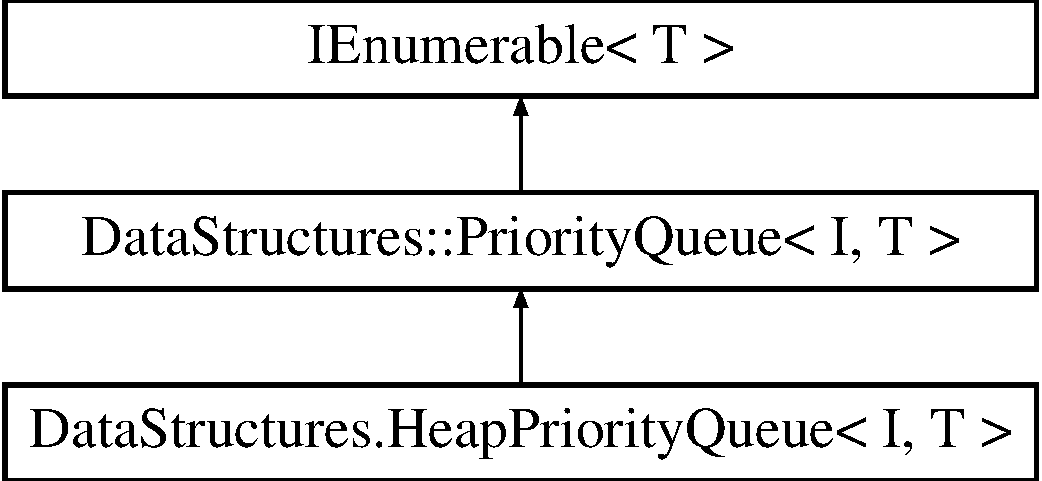
\includegraphics[height=3.000000cm]{class_data_structures_1_1_heap_priority_queue}
\end{center}
\end{figure}
\subsection*{Public Member Functions}
\begin{DoxyCompactItemize}
\item 
\mbox{\Hypertarget{class_data_structures_1_1_heap_priority_queue_a534860c61751a4b72ec6960259f0202e}\label{class_data_structures_1_1_heap_priority_queue_a534860c61751a4b72ec6960259f0202e}} 
{\bfseries Heap\+Priority\+Queue} (int capacity)
\item 
\mbox{\Hypertarget{class_data_structures_1_1_heap_priority_queue_ad591fc63bc6be7028267e66d90f55d22}\label{class_data_structures_1_1_heap_priority_queue_ad591fc63bc6be7028267e66d90f55d22}} 
{\bfseries Heap\+Priority\+Queue} (\hyperlink{class_data_structures_1_1_heap_priority_queue}{Heap\+Priority\+Queue}$<$ I, T $>$ original)
\item 
\mbox{\Hypertarget{class_data_structures_1_1_heap_priority_queue_a00b61bd157c306de51be32441419521b}\label{class_data_structures_1_1_heap_priority_queue_a00b61bd157c306de51be32441419521b}} 
override void {\bfseries Clear} ()
\item 
\mbox{\Hypertarget{class_data_structures_1_1_heap_priority_queue_a09e40d86cc08d7476bb3319e6b37515b}\label{class_data_structures_1_1_heap_priority_queue_a09e40d86cc08d7476bb3319e6b37515b}} 
override T {\bfseries Dequeue} ()
\item 
\mbox{\Hypertarget{class_data_structures_1_1_heap_priority_queue_abc2b3a152c93202b4e3a7cf9292ce9d1}\label{class_data_structures_1_1_heap_priority_queue_abc2b3a152c93202b4e3a7cf9292ce9d1}} 
override T {\bfseries Dequeue} (out I priority)
\item 
\mbox{\Hypertarget{class_data_structures_1_1_heap_priority_queue_abb33bb5d4372b108889f6bf26084860c}\label{class_data_structures_1_1_heap_priority_queue_abb33bb5d4372b108889f6bf26084860c}} 
override I {\bfseries Max\+Priority} ()
\item 
\mbox{\Hypertarget{class_data_structures_1_1_heap_priority_queue_ae76c92ec00718a34dc2c97fc79088d5f}\label{class_data_structures_1_1_heap_priority_queue_ae76c92ec00718a34dc2c97fc79088d5f}} 
override void {\bfseries Enqueue} (T element, I priority)
\item 
\mbox{\Hypertarget{class_data_structures_1_1_heap_priority_queue_a1a494343382d19d56e05302ce33c9104}\label{class_data_structures_1_1_heap_priority_queue_a1a494343382d19d56e05302ce33c9104}} 
override I\+Enumerator$<$ T $>$ {\bfseries Get\+Enumerator} ()
\item 
\mbox{\Hypertarget{class_data_structures_1_1_heap_priority_queue_ab867fe3b8dbbe4635445e0e2209cab57}\label{class_data_structures_1_1_heap_priority_queue_ab867fe3b8dbbe4635445e0e2209cab57}} 
override bool {\bfseries Is\+Empty} ()
\item 
\mbox{\Hypertarget{class_data_structures_1_1_heap_priority_queue_a2ba85a275a772c791c3a3e794a67429c}\label{class_data_structures_1_1_heap_priority_queue_a2ba85a275a772c791c3a3e794a67429c}} 
override T {\bfseries Peek} ()
\item 
\mbox{\Hypertarget{class_data_structures_1_1_heap_priority_queue_ae082d3747d6a2421a34abea334fbb560}\label{class_data_structures_1_1_heap_priority_queue_ae082d3747d6a2421a34abea334fbb560}} 
override void {\bfseries Remove} (T element)
\item 
\mbox{\Hypertarget{class_data_structures_1_1_heap_priority_queue_a8caf23c97ecbbb8ed80c81fa5031fbad}\label{class_data_structures_1_1_heap_priority_queue_a8caf23c97ecbbb8ed80c81fa5031fbad}} 
override void {\bfseries Remove} (T element, I priority)
\end{DoxyCompactItemize}
\subsection*{Properties}
\begin{DoxyCompactItemize}
\item 
\mbox{\Hypertarget{class_data_structures_1_1_heap_priority_queue_a39882f58019d6f6c16702ef5dd16b174}\label{class_data_structures_1_1_heap_priority_queue_a39882f58019d6f6c16702ef5dd16b174}} 
override int {\bfseries Count}\hspace{0.3cm}{\ttfamily  \mbox{[}get\mbox{]}}
\end{DoxyCompactItemize}


The documentation for this class was generated from the following file\+:\begin{DoxyCompactItemize}
\item 
Data\+Structures/Heap\+Priority\+Queue.\+cs\end{DoxyCompactItemize}

\hypertarget{class_data_structures_1_1_list_priority_queue}{}\section{Data\+Structures.\+List\+Priority\+Queue$<$ I, T $>$ Class Template Reference}
\label{class_data_structures_1_1_list_priority_queue}\index{Data\+Structures.\+List\+Priority\+Queue$<$ I, T $>$@{Data\+Structures.\+List\+Priority\+Queue$<$ I, T $>$}}
Inheritance diagram for Data\+Structures.\+List\+Priority\+Queue$<$ I, T $>$\+:\begin{figure}[H]
\begin{center}
\leavevmode
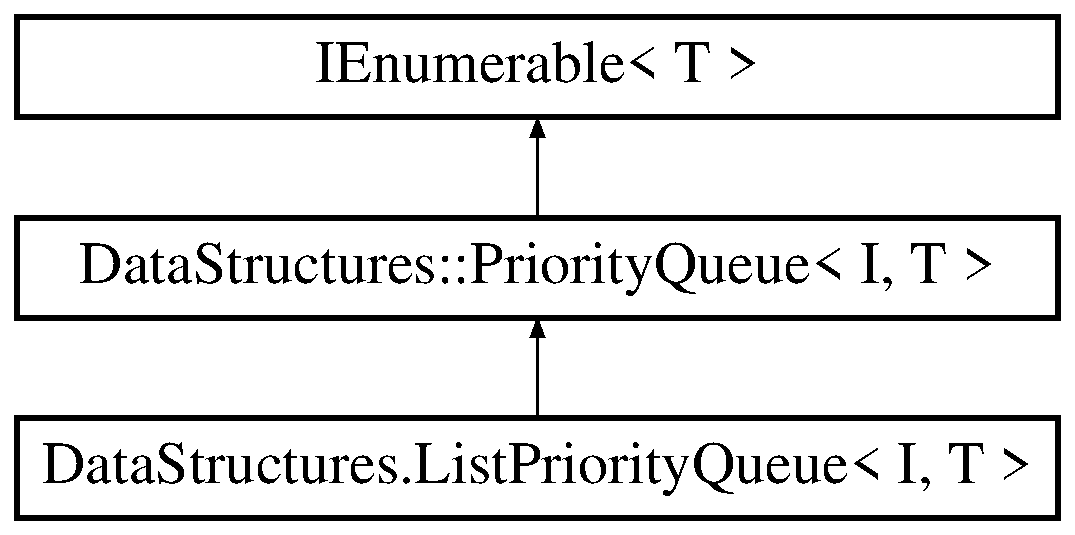
\includegraphics[height=3.000000cm]{class_data_structures_1_1_list_priority_queue}
\end{center}
\end{figure}
\subsection*{Public Member Functions}
\begin{DoxyCompactItemize}
\item 
\mbox{\Hypertarget{class_data_structures_1_1_list_priority_queue_a722492a974e4ae345f8765a6834b8ffb}\label{class_data_structures_1_1_list_priority_queue_a722492a974e4ae345f8765a6834b8ffb}} 
override void {\bfseries Clear} ()
\item 
\mbox{\Hypertarget{class_data_structures_1_1_list_priority_queue_aa4291e0b9ea3a1612682335e80a6b010}\label{class_data_structures_1_1_list_priority_queue_aa4291e0b9ea3a1612682335e80a6b010}} 
override T {\bfseries Dequeue} ()
\item 
\mbox{\Hypertarget{class_data_structures_1_1_list_priority_queue_ac8f364895f67970aaed6dcfaf1290db1}\label{class_data_structures_1_1_list_priority_queue_ac8f364895f67970aaed6dcfaf1290db1}} 
override T {\bfseries Dequeue} (out I priority)
\item 
\mbox{\Hypertarget{class_data_structures_1_1_list_priority_queue_addd32118f7f7876c3d5b3a0757f6863c}\label{class_data_structures_1_1_list_priority_queue_addd32118f7f7876c3d5b3a0757f6863c}} 
override I {\bfseries Max\+Priority} ()
\item 
\mbox{\Hypertarget{class_data_structures_1_1_list_priority_queue_a1538115fa88eb48f79acb5b8c800b6a9}\label{class_data_structures_1_1_list_priority_queue_a1538115fa88eb48f79acb5b8c800b6a9}} 
override T {\bfseries Peek} ()
\item 
\mbox{\Hypertarget{class_data_structures_1_1_list_priority_queue_a7aa8356d1d5029d49bed7824ecaf22e7}\label{class_data_structures_1_1_list_priority_queue_a7aa8356d1d5029d49bed7824ecaf22e7}} 
override void {\bfseries Enqueue} (T element, I priority)
\item 
\mbox{\Hypertarget{class_data_structures_1_1_list_priority_queue_a5e5a94d66964576ff2d0e6b8e3203d8a}\label{class_data_structures_1_1_list_priority_queue_a5e5a94d66964576ff2d0e6b8e3203d8a}} 
override I\+Enumerator$<$ T $>$ {\bfseries Get\+Enumerator} ()
\item 
\mbox{\Hypertarget{class_data_structures_1_1_list_priority_queue_a601185c727c36ac12fca2a3653690a58}\label{class_data_structures_1_1_list_priority_queue_a601185c727c36ac12fca2a3653690a58}} 
override bool {\bfseries Is\+Empty} ()
\item 
\mbox{\Hypertarget{class_data_structures_1_1_list_priority_queue_a8456610791d091dff91553039630607c}\label{class_data_structures_1_1_list_priority_queue_a8456610791d091dff91553039630607c}} 
override void {\bfseries Remove} (T element, I priority)
\item 
\mbox{\Hypertarget{class_data_structures_1_1_list_priority_queue_a2cf5a418704255f9d0f837de6f7fa107}\label{class_data_structures_1_1_list_priority_queue_a2cf5a418704255f9d0f837de6f7fa107}} 
override void {\bfseries Remove} (T element)
\item 
\mbox{\Hypertarget{class_data_structures_1_1_list_priority_queue_a60d2e558bd2110d0d183fb47a5e7d93a}\label{class_data_structures_1_1_list_priority_queue_a60d2e558bd2110d0d183fb47a5e7d93a}} 
T {\bfseries Pop} ()
\end{DoxyCompactItemize}
\subsection*{Properties}
\begin{DoxyCompactItemize}
\item 
\mbox{\Hypertarget{class_data_structures_1_1_list_priority_queue_a7bc9b2551d95ed8d9a56376d2098e4eb}\label{class_data_structures_1_1_list_priority_queue_a7bc9b2551d95ed8d9a56376d2098e4eb}} 
override int {\bfseries Count}\hspace{0.3cm}{\ttfamily  \mbox{[}get\mbox{]}}
\end{DoxyCompactItemize}


The documentation for this class was generated from the following file\+:\begin{DoxyCompactItemize}
\item 
Data\+Structures/List\+Priority\+Queue.\+cs\end{DoxyCompactItemize}

\hypertarget{struct_loading_1_1_loading_priority}{}\section{Loading.\+Loading\+Priority Struct Reference}
\label{struct_loading_1_1_loading_priority}\index{Loading.\+Loading\+Priority@{Loading.\+Loading\+Priority}}
Inheritance diagram for Loading.\+Loading\+Priority\+:\begin{figure}[H]
\begin{center}
\leavevmode
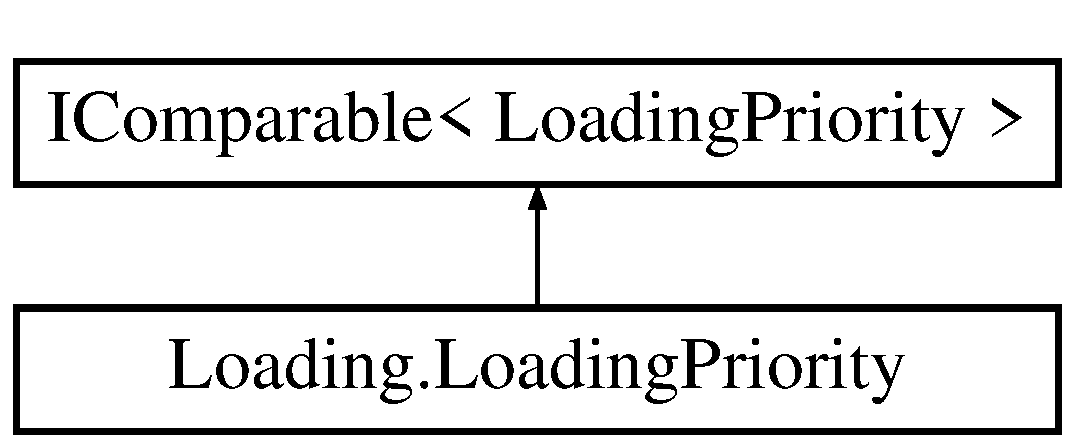
\includegraphics[height=2.000000cm]{struct_loading_1_1_loading_priority}
\end{center}
\end{figure}
\subsection*{Public Member Functions}
\begin{DoxyCompactItemize}
\item 
\mbox{\Hypertarget{struct_loading_1_1_loading_priority_a598efdfb29010f81259575c1b5b6a4bc}\label{struct_loading_1_1_loading_priority_a598efdfb29010f81259575c1b5b6a4bc}} 
{\bfseries Loading\+Priority} (\hyperlink{class_cloud_data_1_1_point_cloud_meta_data}{Point\+Cloud\+Meta\+Data} cloud, string node\+Name, double calculated\+Priority, bool invert)
\item 
\mbox{\Hypertarget{struct_loading_1_1_loading_priority_a953a6e0248f7224fe88ec1eca46c832d}\label{struct_loading_1_1_loading_priority_a953a6e0248f7224fe88ec1eca46c832d}} 
int {\bfseries Compare\+To} (\hyperlink{struct_loading_1_1_loading_priority}{Loading\+Priority} other)
\end{DoxyCompactItemize}
\subsection*{Static Public Member Functions}
\begin{DoxyCompactItemize}
\item 
\mbox{\Hypertarget{struct_loading_1_1_loading_priority_a1334e418137649e7ff008fe08eb41f3d}\label{struct_loading_1_1_loading_priority_a1334e418137649e7ff008fe08eb41f3d}} 
static bool {\bfseries operator$<$} (\hyperlink{struct_loading_1_1_loading_priority}{Loading\+Priority} a, \hyperlink{struct_loading_1_1_loading_priority}{Loading\+Priority} b)
\item 
\mbox{\Hypertarget{struct_loading_1_1_loading_priority_ab5fd0b00e75e50839a0d3ddfe115112c}\label{struct_loading_1_1_loading_priority_ab5fd0b00e75e50839a0d3ddfe115112c}} 
static bool {\bfseries operator$>$} (\hyperlink{struct_loading_1_1_loading_priority}{Loading\+Priority} a, \hyperlink{struct_loading_1_1_loading_priority}{Loading\+Priority} b)
\item 
\mbox{\Hypertarget{struct_loading_1_1_loading_priority_a5edd56d05daf22b47d1d6375627f3487}\label{struct_loading_1_1_loading_priority_a5edd56d05daf22b47d1d6375627f3487}} 
static \hyperlink{struct_loading_1_1_loading_priority}{Loading\+Priority} {\bfseries operator-\/} (\hyperlink{struct_loading_1_1_loading_priority}{Loading\+Priority} p)
\end{DoxyCompactItemize}
\subsection*{Public Attributes}
\begin{DoxyCompactItemize}
\item 
\mbox{\Hypertarget{struct_loading_1_1_loading_priority_a27bfeb4785cc81c21b372bdcc5b9bb8e}\label{struct_loading_1_1_loading_priority_a27bfeb4785cc81c21b372bdcc5b9bb8e}} 
readonly \hyperlink{class_cloud_data_1_1_point_cloud_meta_data}{Point\+Cloud\+Meta\+Data} {\bfseries cloud}
\item 
\mbox{\Hypertarget{struct_loading_1_1_loading_priority_ae0f94ed4d076a7c133d578a19de02734}\label{struct_loading_1_1_loading_priority_ae0f94ed4d076a7c133d578a19de02734}} 
readonly string {\bfseries node\+Name}
\item 
\mbox{\Hypertarget{struct_loading_1_1_loading_priority_a9bafe1ba3ebb9c10188b9cd5d0f09faf}\label{struct_loading_1_1_loading_priority_a9bafe1ba3ebb9c10188b9cd5d0f09faf}} 
readonly double {\bfseries calculated\+Priority}
\item 
\mbox{\Hypertarget{struct_loading_1_1_loading_priority_a3e1cca3f2f6b39cb1f213754a45f2541}\label{struct_loading_1_1_loading_priority_a3e1cca3f2f6b39cb1f213754a45f2541}} 
readonly int {\bfseries invert}
\end{DoxyCompactItemize}


The documentation for this struct was generated from the following file\+:\begin{DoxyCompactItemize}
\item 
Loading/Loading\+Priority.\+cs\end{DoxyCompactItemize}

\hypertarget{class_object_creation_1_1_mesh_configuration}{}\section{Object\+Creation.\+Mesh\+Configuration Class Reference}
\label{class_object_creation_1_1_mesh_configuration}\index{Object\+Creation.\+Mesh\+Configuration@{Object\+Creation.\+Mesh\+Configuration}}
Inheritance diagram for Object\+Creation.\+Mesh\+Configuration\+:\begin{figure}[H]
\begin{center}
\leavevmode
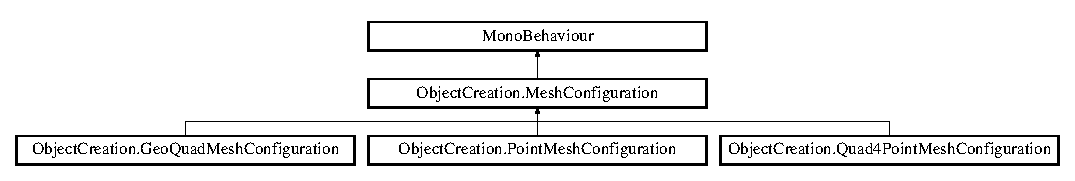
\includegraphics[height=1.985816cm]{class_object_creation_1_1_mesh_configuration}
\end{center}
\end{figure}
\subsection*{Public Member Functions}
\begin{DoxyCompactItemize}
\item 
\mbox{\Hypertarget{class_object_creation_1_1_mesh_configuration_ad5c68a195c3dcf49d75b3b6d57765265}\label{class_object_creation_1_1_mesh_configuration_ad5c68a195c3dcf49d75b3b6d57765265}} 
abstract int {\bfseries Get\+Maximum\+Points\+Per\+Mesh} ()
\item 
\mbox{\Hypertarget{class_object_creation_1_1_mesh_configuration_a23fa629a42465c46ab797169344c233c}\label{class_object_creation_1_1_mesh_configuration_a23fa629a42465c46ab797169344c233c}} 
abstract Game\+Object {\bfseries Create\+Game\+Object} (string name, Vector3\mbox{[}$\,$\mbox{]} vertex\+Data, Color\mbox{[}$\,$\mbox{]} color\+Data, \hyperlink{class_cloud_data_1_1_bounding_box}{Bounding\+Box} bounding\+Box)
\item 
\mbox{\Hypertarget{class_object_creation_1_1_mesh_configuration_ad6658e84abae937703fdad3b7e64de6e}\label{class_object_creation_1_1_mesh_configuration_ad6658e84abae937703fdad3b7e64de6e}} 
abstract void {\bfseries Remove\+Game\+Object} (Game\+Object game\+Object)
\end{DoxyCompactItemize}


The documentation for this class was generated from the following file\+:\begin{DoxyCompactItemize}
\item 
Object\+Creation/Mesh\+Configuration.\+cs\end{DoxyCompactItemize}

\hypertarget{class_cloud_data_1_1_node}{}\section{Cloud\+Data.\+Node Class Reference}
\label{class_cloud_data_1_1_node}\index{Cloud\+Data.\+Node@{Cloud\+Data.\+Node}}


Resembles a node of the nested octree.  


Inheritance diagram for Cloud\+Data.\+Node\+:\begin{figure}[H]
\begin{center}
\leavevmode
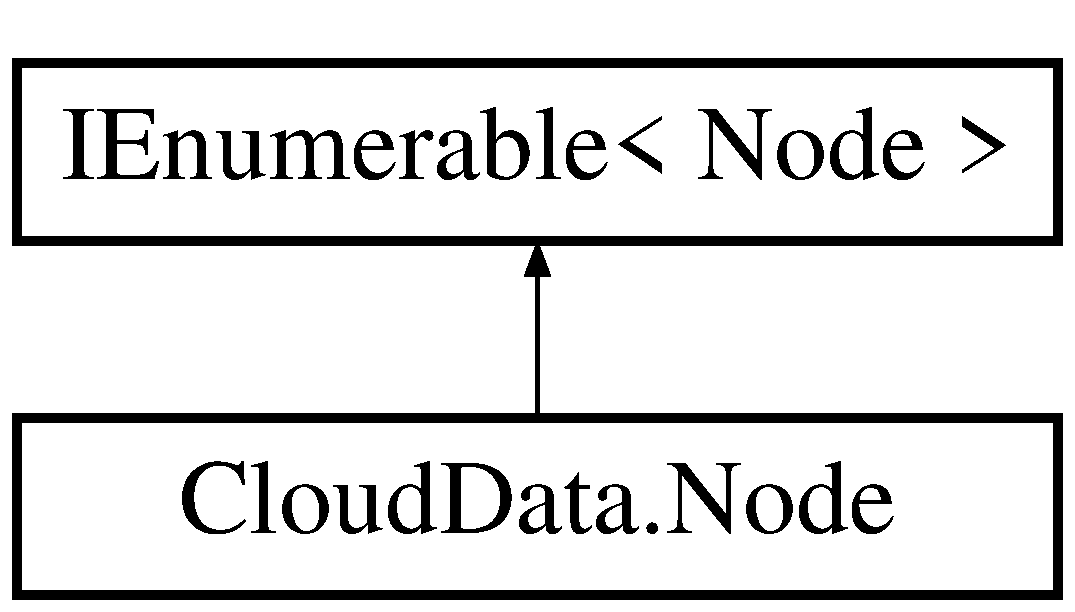
\includegraphics[height=2.000000cm]{class_cloud_data_1_1_node}
\end{center}
\end{figure}
\subsection*{Public Member Functions}
\begin{DoxyCompactItemize}
\item 
\hyperlink{class_cloud_data_1_1_node_a6540b5d8cb8fc40067560b3c002d574c}{Node} (string name, \hyperlink{class_cloud_data_1_1_point_cloud_meta_data}{Point\+Cloud\+Meta\+Data} meta\+Data, \hyperlink{class_cloud_data_1_1_bounding_box}{Bounding\+Box} bounding\+Box, \hyperlink{class_cloud_data_1_1_node}{Node} parent)
\begin{DoxyCompactList}\small\item\em Creates a new node object. \end{DoxyCompactList}\item 
int \hyperlink{class_cloud_data_1_1_node_af70f14b2486f62d63e1155a1a7d4f34f}{Get\+Level} ()
\begin{DoxyCompactList}\small\item\em Returns how deep in the tree this node is. 0 means it is the root node, 1 means it is a child of the root node and so on... \end{DoxyCompactList}\item 
void \hyperlink{class_cloud_data_1_1_node_a5d81b4c9928dbdc1d204c13feb645da0}{Create\+Game\+Objects} (\hyperlink{class_object_creation_1_1_mesh_configuration}{Mesh\+Configuration} configuration)
\begin{DoxyCompactList}\small\item\em Creates the Game Object(s) containing the points of this node. Vertices and Colors have to be set before calling this function (via Set\+Points)! This function has to be called from the main thread! \end{DoxyCompactList}\item 
Game\+Object \hyperlink{class_cloud_data_1_1_node_a79ada8b9a0cf64c7d23f70b862681f4c}{Create\+Bounding\+Box\+Game\+Object} ()
\begin{DoxyCompactList}\small\item\em Creates a transparent box game object with the shape of the bounding box of this node. The color is determined by the hashcode of this node. Used for debugging purposes only. \end{DoxyCompactList}\item 
void \hyperlink{class_cloud_data_1_1_node_a75101ac753ab2b540c0a1f8e761f79df}{Create\+All\+Game\+Objects} (\hyperlink{class_object_creation_1_1_mesh_configuration}{Mesh\+Configuration} configuration)
\begin{DoxyCompactList}\small\item\em Creates Game\+Objects for this node and all its (grand-\/)children. Useable for displaying a whole point cloud at once. Vertices and Colors have to be set before calling this function (via Set\+Points) for this object and all its children! This function has to be called from the main thread! \end{DoxyCompactList}\item 
void \hyperlink{class_cloud_data_1_1_node_a98647399470b2adc5c6ac27ca78c5ddb}{Remove\+Game\+Objects} (\hyperlink{class_object_creation_1_1_mesh_configuration}{Mesh\+Configuration} config)
\begin{DoxyCompactList}\small\item\em Removes the Game\+Objects of this node. Has to be called from the main thread. \end{DoxyCompactList}\item 
void \hyperlink{class_cloud_data_1_1_node_a397ec14bfc75899441b6edfcabb004ad}{Deactivate\+Game\+Objects} ()
\begin{DoxyCompactList}\small\item\em Deactivates the Game\+Objects of this node. Has to be called from the main thread. \end{DoxyCompactList}\item 
void \hyperlink{class_cloud_data_1_1_node_a8a7c01462a603882108e401c8119e388}{Reactivate\+Game\+Objects} ()
\begin{DoxyCompactList}\small\item\em Activates the Game\+Objects of this node (Game\+Objects are usually active after creation. A call of this function only makes sense after previously calling Deactivate\+Game\+Objects). Has to be called from the main thread. \end{DoxyCompactList}\item 
bool \hyperlink{class_cloud_data_1_1_node_aeb88a03cff66169770082a2e72a9f326}{Are\+Game\+Objects\+Active} ()
\begin{DoxyCompactList}\small\item\em Returns true, iff there are Game Objects and they are active OR there are not Game Objects for this object. \end{DoxyCompactList}\item 
void \hyperlink{class_cloud_data_1_1_node_af82be4d0f143e8894ec6d2ecf4ae8c31}{Set\+Points} (Vector3\mbox{[}$\,$\mbox{]} vertices, Color\mbox{[}$\,$\mbox{]} colors)
\begin{DoxyCompactList}\small\item\em Sets the point data. Throws an exception if gameobjects already exist or vertices or colors are null or their length do not match. Also sets the point count. \end{DoxyCompactList}\item 
void \hyperlink{class_cloud_data_1_1_node_a42cf1e1f98f40a542173abce2b82a078}{Forget\+Points} ()
\begin{DoxyCompactList}\small\item\em Deletes the loaded vertex-\/ and color-\/information (to release the used memory). The point count stays saved however. \end{DoxyCompactList}\item 
bool \hyperlink{class_cloud_data_1_1_node_add8b3fc44e4abc6572f7a723deda352d}{Has\+Points\+To\+Render} ()
\begin{DoxyCompactList}\small\item\em Returns true, iff vertices and colors are set \end{DoxyCompactList}\item 
bool \hyperlink{class_cloud_data_1_1_node_aa253c61651daa14e2377ddb189f56320}{Has\+Game\+Objects} ()
\begin{DoxyCompactList}\small\item\em Returns true, iff this object has Game\+Objects. \end{DoxyCompactList}\item 
void \hyperlink{class_cloud_data_1_1_node_aa4164d93a7380b4f3704c0ac36663164}{Set\+Child} (int index, \hyperlink{class_cloud_data_1_1_node}{Node} node)
\begin{DoxyCompactList}\small\item\em Sets the child with the given index \end{DoxyCompactList}\item 
\hyperlink{class_cloud_data_1_1_node}{Node} \hyperlink{class_cloud_data_1_1_node_a93ba39401d22c904ec3a9631fca1c222}{Get\+Child} (int index)
\begin{DoxyCompactList}\small\item\em Returns the child at the given index \end{DoxyCompactList}\item 
bool \hyperlink{class_cloud_data_1_1_node_a42e31008a7772d196ce770ff2244cc26}{Has\+Child} (int index)
\begin{DoxyCompactList}\small\item\em Returns true, iff the node has a child at the given index. \end{DoxyCompactList}\item 
I\+Enumerator$<$ \hyperlink{class_cloud_data_1_1_node}{Node} $>$ \hyperlink{class_cloud_data_1_1_node_adbc0168d2d1b1c9600c2f91720f00c18}{Get\+Enumerator} ()
\begin{DoxyCompactList}\small\item\em Returns an enumerator with which it is possible to enumerate through the children of the node (not including null-\/values) \end{DoxyCompactList}\item 
override string \hyperlink{class_cloud_data_1_1_node_af070c6770edc822d95393383c70aa055}{To\+String} ()
\begin{DoxyCompactList}\small\item\em Returns a string representation of the \hyperlink{class_cloud_data_1_1_node}{Node} (for example \char`\"{}\+Node\+: r123\char`\"{}) \end{DoxyCompactList}\end{DoxyCompactItemize}
\subsection*{Properties}
\begin{DoxyCompactItemize}
\item 
string \hyperlink{class_cloud_data_1_1_node_ad6676243e485f19675af4055c164071b}{Name}\hspace{0.3cm}{\ttfamily  \mbox{[}get\mbox{]}}
\begin{DoxyCompactList}\small\item\em The name of the node, which is the path of the node in the tree. For example \char`\"{}023\char`\"{} for the forth child of the third child of the first child of the root node. (readonly) \end{DoxyCompactList}\item 
\hyperlink{class_cloud_data_1_1_bounding_box}{Bounding\+Box} \hyperlink{class_cloud_data_1_1_node_ad82330bd7fb62f8c25512d2f3ecd7888}{Bounding\+Box}\hspace{0.3cm}{\ttfamily  \mbox{[}get\mbox{]}}
\begin{DoxyCompactList}\small\item\em The \hyperlink{class_cloud_data_1_1_bounding_box}{Bounding\+Box} of the node (readonly) \end{DoxyCompactList}\item 
\hyperlink{class_cloud_data_1_1_node}{Node} \hyperlink{class_cloud_data_1_1_node_ae7600b8769acc09e7d3a6d4a5382fed8}{Parent}\hspace{0.3cm}{\ttfamily  \mbox{[}get, set\mbox{]}}
\begin{DoxyCompactList}\small\item\em The parent of this node (may be null, if this is a root node) \end{DoxyCompactList}\item 
int \hyperlink{class_cloud_data_1_1_node_a5d9df7ed9ea8c45472d032591e7ea99c}{Point\+Count}\hspace{0.3cm}{\ttfamily  \mbox{[}get\mbox{]}}
\begin{DoxyCompactList}\small\item\em Number of points given the last time Set\+Points was called. Or -\/1 if it hasn\textquotesingle{}t been called yet \end{DoxyCompactList}\item 
\hyperlink{class_cloud_data_1_1_point_cloud_meta_data}{Point\+Cloud\+Meta\+Data} \hyperlink{class_cloud_data_1_1_node_acc0afd56fb7f3c0c22fdfda9c43dce0c}{Meta\+Data}\hspace{0.3cm}{\ttfamily  \mbox{[}get\mbox{]}}
\begin{DoxyCompactList}\small\item\em The metadata identifying which pointcloud this node belongs to \end{DoxyCompactList}\item 
byte \hyperlink{class_cloud_data_1_1_node_add6b3b455a1b95a74506a849a1081f28}{Node\+Status}\hspace{0.3cm}{\ttfamily  \mbox{[}get, set\mbox{]}}
\begin{DoxyCompactList}\small\item\em The status of this node. The meaning and use of the \hyperlink{class_cloud_data_1_1_node_status}{Node\+Status} is dependent from the used renderer and does not have to be used consistently by all renders. Currently its only used by the Concurrent\+Multi\+Time\+Renderer. \end{DoxyCompactList}\end{DoxyCompactItemize}


\subsection{Detailed Description}
Resembles a node of the nested octree. 



\subsection{Constructor \& Destructor Documentation}
\mbox{\Hypertarget{class_cloud_data_1_1_node_a6540b5d8cb8fc40067560b3c002d574c}\label{class_cloud_data_1_1_node_a6540b5d8cb8fc40067560b3c002d574c}} 
\index{Cloud\+Data\+::\+Node@{Cloud\+Data\+::\+Node}!Node@{Node}}
\index{Node@{Node}!Cloud\+Data\+::\+Node@{Cloud\+Data\+::\+Node}}
\subsubsection{\texorpdfstring{Node()}{Node()}}
{\footnotesize\ttfamily Cloud\+Data.\+Node.\+Node (\begin{DoxyParamCaption}\item[{string}]{name,  }\item[{\hyperlink{class_cloud_data_1_1_point_cloud_meta_data}{Point\+Cloud\+Meta\+Data}}]{meta\+Data,  }\item[{\hyperlink{class_cloud_data_1_1_bounding_box}{Bounding\+Box}}]{bounding\+Box,  }\item[{\hyperlink{class_cloud_data_1_1_node}{Node}}]{parent }\end{DoxyParamCaption})\hspace{0.3cm}{\ttfamily [inline]}}



Creates a new node object. 


\begin{DoxyParams}{Parameters}
{\em name} & The path of the node in the tree. For example \char`\"{}023\char`\"{} for the forth child of the third child of the first child of the root node.\\
\hline
{\em meta\+Data} & The meta data of the point cloud, to identify which cloud this node belongs to.\\
\hline
{\em bounding\+Box} & The bounding box of this node.\\
\hline
{\em parent} & The parent node. May be null if this is the root node.\\
\hline
\end{DoxyParams}


\subsection{Member Function Documentation}
\mbox{\Hypertarget{class_cloud_data_1_1_node_aeb88a03cff66169770082a2e72a9f326}\label{class_cloud_data_1_1_node_aeb88a03cff66169770082a2e72a9f326}} 
\index{Cloud\+Data\+::\+Node@{Cloud\+Data\+::\+Node}!Are\+Game\+Objects\+Active@{Are\+Game\+Objects\+Active}}
\index{Are\+Game\+Objects\+Active@{Are\+Game\+Objects\+Active}!Cloud\+Data\+::\+Node@{Cloud\+Data\+::\+Node}}
\subsubsection{\texorpdfstring{Are\+Game\+Objects\+Active()}{AreGameObjectsActive()}}
{\footnotesize\ttfamily bool Cloud\+Data.\+Node.\+Are\+Game\+Objects\+Active (\begin{DoxyParamCaption}{ }\end{DoxyParamCaption})\hspace{0.3cm}{\ttfamily [inline]}}



Returns true, iff there are Game Objects and they are active OR there are not Game Objects for this object. 

\mbox{\Hypertarget{class_cloud_data_1_1_node_a75101ac753ab2b540c0a1f8e761f79df}\label{class_cloud_data_1_1_node_a75101ac753ab2b540c0a1f8e761f79df}} 
\index{Cloud\+Data\+::\+Node@{Cloud\+Data\+::\+Node}!Create\+All\+Game\+Objects@{Create\+All\+Game\+Objects}}
\index{Create\+All\+Game\+Objects@{Create\+All\+Game\+Objects}!Cloud\+Data\+::\+Node@{Cloud\+Data\+::\+Node}}
\subsubsection{\texorpdfstring{Create\+All\+Game\+Objects()}{CreateAllGameObjects()}}
{\footnotesize\ttfamily void Cloud\+Data.\+Node.\+Create\+All\+Game\+Objects (\begin{DoxyParamCaption}\item[{\hyperlink{class_object_creation_1_1_mesh_configuration}{Mesh\+Configuration}}]{configuration }\end{DoxyParamCaption})\hspace{0.3cm}{\ttfamily [inline]}}



Creates Game\+Objects for this node and all its (grand-\/)children. Useable for displaying a whole point cloud at once. Vertices and Colors have to be set before calling this function (via Set\+Points) for this object and all its children! This function has to be called from the main thread! 


\begin{DoxyParams}{Parameters}
{\em configuration} & The Mesh\+Configuration which should be used for creating the Game Objects\\
\hline
\end{DoxyParams}
\mbox{\Hypertarget{class_cloud_data_1_1_node_a79ada8b9a0cf64c7d23f70b862681f4c}\label{class_cloud_data_1_1_node_a79ada8b9a0cf64c7d23f70b862681f4c}} 
\index{Cloud\+Data\+::\+Node@{Cloud\+Data\+::\+Node}!Create\+Bounding\+Box\+Game\+Object@{Create\+Bounding\+Box\+Game\+Object}}
\index{Create\+Bounding\+Box\+Game\+Object@{Create\+Bounding\+Box\+Game\+Object}!Cloud\+Data\+::\+Node@{Cloud\+Data\+::\+Node}}
\subsubsection{\texorpdfstring{Create\+Bounding\+Box\+Game\+Object()}{CreateBoundingBoxGameObject()}}
{\footnotesize\ttfamily Game\+Object Cloud\+Data.\+Node.\+Create\+Bounding\+Box\+Game\+Object (\begin{DoxyParamCaption}{ }\end{DoxyParamCaption})\hspace{0.3cm}{\ttfamily [inline]}}



Creates a transparent box game object with the shape of the bounding box of this node. The color is determined by the hashcode of this node. Used for debugging purposes only. 

\mbox{\Hypertarget{class_cloud_data_1_1_node_a5d81b4c9928dbdc1d204c13feb645da0}\label{class_cloud_data_1_1_node_a5d81b4c9928dbdc1d204c13feb645da0}} 
\index{Cloud\+Data\+::\+Node@{Cloud\+Data\+::\+Node}!Create\+Game\+Objects@{Create\+Game\+Objects}}
\index{Create\+Game\+Objects@{Create\+Game\+Objects}!Cloud\+Data\+::\+Node@{Cloud\+Data\+::\+Node}}
\subsubsection{\texorpdfstring{Create\+Game\+Objects()}{CreateGameObjects()}}
{\footnotesize\ttfamily void Cloud\+Data.\+Node.\+Create\+Game\+Objects (\begin{DoxyParamCaption}\item[{\hyperlink{class_object_creation_1_1_mesh_configuration}{Mesh\+Configuration}}]{configuration }\end{DoxyParamCaption})\hspace{0.3cm}{\ttfamily [inline]}}



Creates the Game Object(s) containing the points of this node. Vertices and Colors have to be set before calling this function (via Set\+Points)! This function has to be called from the main thread! 


\begin{DoxyParams}{Parameters}
{\em configuration} & The Mesh\+Configuration which should be used for creating the Game Objects\\
\hline
\end{DoxyParams}
\mbox{\Hypertarget{class_cloud_data_1_1_node_a397ec14bfc75899441b6edfcabb004ad}\label{class_cloud_data_1_1_node_a397ec14bfc75899441b6edfcabb004ad}} 
\index{Cloud\+Data\+::\+Node@{Cloud\+Data\+::\+Node}!Deactivate\+Game\+Objects@{Deactivate\+Game\+Objects}}
\index{Deactivate\+Game\+Objects@{Deactivate\+Game\+Objects}!Cloud\+Data\+::\+Node@{Cloud\+Data\+::\+Node}}
\subsubsection{\texorpdfstring{Deactivate\+Game\+Objects()}{DeactivateGameObjects()}}
{\footnotesize\ttfamily void Cloud\+Data.\+Node.\+Deactivate\+Game\+Objects (\begin{DoxyParamCaption}{ }\end{DoxyParamCaption})\hspace{0.3cm}{\ttfamily [inline]}}



Deactivates the Game\+Objects of this node. Has to be called from the main thread. 

\mbox{\Hypertarget{class_cloud_data_1_1_node_a42cf1e1f98f40a542173abce2b82a078}\label{class_cloud_data_1_1_node_a42cf1e1f98f40a542173abce2b82a078}} 
\index{Cloud\+Data\+::\+Node@{Cloud\+Data\+::\+Node}!Forget\+Points@{Forget\+Points}}
\index{Forget\+Points@{Forget\+Points}!Cloud\+Data\+::\+Node@{Cloud\+Data\+::\+Node}}
\subsubsection{\texorpdfstring{Forget\+Points()}{ForgetPoints()}}
{\footnotesize\ttfamily void Cloud\+Data.\+Node.\+Forget\+Points (\begin{DoxyParamCaption}{ }\end{DoxyParamCaption})\hspace{0.3cm}{\ttfamily [inline]}}



Deletes the loaded vertex-\/ and color-\/information (to release the used memory). The point count stays saved however. 

\mbox{\Hypertarget{class_cloud_data_1_1_node_a93ba39401d22c904ec3a9631fca1c222}\label{class_cloud_data_1_1_node_a93ba39401d22c904ec3a9631fca1c222}} 
\index{Cloud\+Data\+::\+Node@{Cloud\+Data\+::\+Node}!Get\+Child@{Get\+Child}}
\index{Get\+Child@{Get\+Child}!Cloud\+Data\+::\+Node@{Cloud\+Data\+::\+Node}}
\subsubsection{\texorpdfstring{Get\+Child()}{GetChild()}}
{\footnotesize\ttfamily \hyperlink{class_cloud_data_1_1_node}{Node} Cloud\+Data.\+Node.\+Get\+Child (\begin{DoxyParamCaption}\item[{int}]{index }\end{DoxyParamCaption})\hspace{0.3cm}{\ttfamily [inline]}}



Returns the child at the given index 


\begin{DoxyParams}{Parameters}
{\em index} & 0 $<$= index $<$ 8\\
\hline
\end{DoxyParams}
\begin{DoxyReturn}{Returns}
The child (may be null, if no child exists at that index)
\end{DoxyReturn}
\mbox{\Hypertarget{class_cloud_data_1_1_node_adbc0168d2d1b1c9600c2f91720f00c18}\label{class_cloud_data_1_1_node_adbc0168d2d1b1c9600c2f91720f00c18}} 
\index{Cloud\+Data\+::\+Node@{Cloud\+Data\+::\+Node}!Get\+Enumerator@{Get\+Enumerator}}
\index{Get\+Enumerator@{Get\+Enumerator}!Cloud\+Data\+::\+Node@{Cloud\+Data\+::\+Node}}
\subsubsection{\texorpdfstring{Get\+Enumerator()}{GetEnumerator()}}
{\footnotesize\ttfamily I\+Enumerator$<$\hyperlink{class_cloud_data_1_1_node}{Node}$>$ Cloud\+Data.\+Node.\+Get\+Enumerator (\begin{DoxyParamCaption}{ }\end{DoxyParamCaption})\hspace{0.3cm}{\ttfamily [inline]}}



Returns an enumerator with which it is possible to enumerate through the children of the node (not including null-\/values) 

\begin{DoxyReturn}{Returns}

\end{DoxyReturn}
\mbox{\Hypertarget{class_cloud_data_1_1_node_af70f14b2486f62d63e1155a1a7d4f34f}\label{class_cloud_data_1_1_node_af70f14b2486f62d63e1155a1a7d4f34f}} 
\index{Cloud\+Data\+::\+Node@{Cloud\+Data\+::\+Node}!Get\+Level@{Get\+Level}}
\index{Get\+Level@{Get\+Level}!Cloud\+Data\+::\+Node@{Cloud\+Data\+::\+Node}}
\subsubsection{\texorpdfstring{Get\+Level()}{GetLevel()}}
{\footnotesize\ttfamily int Cloud\+Data.\+Node.\+Get\+Level (\begin{DoxyParamCaption}{ }\end{DoxyParamCaption})\hspace{0.3cm}{\ttfamily [inline]}}



Returns how deep in the tree this node is. 0 means it is the root node, 1 means it is a child of the root node and so on... 

\begin{DoxyReturn}{Returns}
the level in the tree ($>$=0)
\end{DoxyReturn}
\mbox{\Hypertarget{class_cloud_data_1_1_node_a42e31008a7772d196ce770ff2244cc26}\label{class_cloud_data_1_1_node_a42e31008a7772d196ce770ff2244cc26}} 
\index{Cloud\+Data\+::\+Node@{Cloud\+Data\+::\+Node}!Has\+Child@{Has\+Child}}
\index{Has\+Child@{Has\+Child}!Cloud\+Data\+::\+Node@{Cloud\+Data\+::\+Node}}
\subsubsection{\texorpdfstring{Has\+Child()}{HasChild()}}
{\footnotesize\ttfamily bool Cloud\+Data.\+Node.\+Has\+Child (\begin{DoxyParamCaption}\item[{int}]{index }\end{DoxyParamCaption})\hspace{0.3cm}{\ttfamily [inline]}}



Returns true, iff the node has a child at the given index. 


\begin{DoxyParams}{Parameters}
{\em index} & 0 $<$= index $<$ 8\\
\hline
\end{DoxyParams}
\mbox{\Hypertarget{class_cloud_data_1_1_node_aa253c61651daa14e2377ddb189f56320}\label{class_cloud_data_1_1_node_aa253c61651daa14e2377ddb189f56320}} 
\index{Cloud\+Data\+::\+Node@{Cloud\+Data\+::\+Node}!Has\+Game\+Objects@{Has\+Game\+Objects}}
\index{Has\+Game\+Objects@{Has\+Game\+Objects}!Cloud\+Data\+::\+Node@{Cloud\+Data\+::\+Node}}
\subsubsection{\texorpdfstring{Has\+Game\+Objects()}{HasGameObjects()}}
{\footnotesize\ttfamily bool Cloud\+Data.\+Node.\+Has\+Game\+Objects (\begin{DoxyParamCaption}{ }\end{DoxyParamCaption})\hspace{0.3cm}{\ttfamily [inline]}}



Returns true, iff this object has Game\+Objects. 

\mbox{\Hypertarget{class_cloud_data_1_1_node_add8b3fc44e4abc6572f7a723deda352d}\label{class_cloud_data_1_1_node_add8b3fc44e4abc6572f7a723deda352d}} 
\index{Cloud\+Data\+::\+Node@{Cloud\+Data\+::\+Node}!Has\+Points\+To\+Render@{Has\+Points\+To\+Render}}
\index{Has\+Points\+To\+Render@{Has\+Points\+To\+Render}!Cloud\+Data\+::\+Node@{Cloud\+Data\+::\+Node}}
\subsubsection{\texorpdfstring{Has\+Points\+To\+Render()}{HasPointsToRender()}}
{\footnotesize\ttfamily bool Cloud\+Data.\+Node.\+Has\+Points\+To\+Render (\begin{DoxyParamCaption}{ }\end{DoxyParamCaption})\hspace{0.3cm}{\ttfamily [inline]}}



Returns true, iff vertices and colors are set 

\mbox{\Hypertarget{class_cloud_data_1_1_node_a8a7c01462a603882108e401c8119e388}\label{class_cloud_data_1_1_node_a8a7c01462a603882108e401c8119e388}} 
\index{Cloud\+Data\+::\+Node@{Cloud\+Data\+::\+Node}!Reactivate\+Game\+Objects@{Reactivate\+Game\+Objects}}
\index{Reactivate\+Game\+Objects@{Reactivate\+Game\+Objects}!Cloud\+Data\+::\+Node@{Cloud\+Data\+::\+Node}}
\subsubsection{\texorpdfstring{Reactivate\+Game\+Objects()}{ReactivateGameObjects()}}
{\footnotesize\ttfamily void Cloud\+Data.\+Node.\+Reactivate\+Game\+Objects (\begin{DoxyParamCaption}{ }\end{DoxyParamCaption})\hspace{0.3cm}{\ttfamily [inline]}}



Activates the Game\+Objects of this node (Game\+Objects are usually active after creation. A call of this function only makes sense after previously calling Deactivate\+Game\+Objects). Has to be called from the main thread. 

\mbox{\Hypertarget{class_cloud_data_1_1_node_a98647399470b2adc5c6ac27ca78c5ddb}\label{class_cloud_data_1_1_node_a98647399470b2adc5c6ac27ca78c5ddb}} 
\index{Cloud\+Data\+::\+Node@{Cloud\+Data\+::\+Node}!Remove\+Game\+Objects@{Remove\+Game\+Objects}}
\index{Remove\+Game\+Objects@{Remove\+Game\+Objects}!Cloud\+Data\+::\+Node@{Cloud\+Data\+::\+Node}}
\subsubsection{\texorpdfstring{Remove\+Game\+Objects()}{RemoveGameObjects()}}
{\footnotesize\ttfamily void Cloud\+Data.\+Node.\+Remove\+Game\+Objects (\begin{DoxyParamCaption}\item[{\hyperlink{class_object_creation_1_1_mesh_configuration}{Mesh\+Configuration}}]{config }\end{DoxyParamCaption})\hspace{0.3cm}{\ttfamily [inline]}}



Removes the Game\+Objects of this node. Has to be called from the main thread. 


\begin{DoxyParams}{Parameters}
{\em config} & The Mesh\+Configuration which should be used for removing the Game Objects\\
\hline
\end{DoxyParams}
\mbox{\Hypertarget{class_cloud_data_1_1_node_aa4164d93a7380b4f3704c0ac36663164}\label{class_cloud_data_1_1_node_aa4164d93a7380b4f3704c0ac36663164}} 
\index{Cloud\+Data\+::\+Node@{Cloud\+Data\+::\+Node}!Set\+Child@{Set\+Child}}
\index{Set\+Child@{Set\+Child}!Cloud\+Data\+::\+Node@{Cloud\+Data\+::\+Node}}
\subsubsection{\texorpdfstring{Set\+Child()}{SetChild()}}
{\footnotesize\ttfamily void Cloud\+Data.\+Node.\+Set\+Child (\begin{DoxyParamCaption}\item[{int}]{index,  }\item[{\hyperlink{class_cloud_data_1_1_node}{Node}}]{node }\end{DoxyParamCaption})\hspace{0.3cm}{\ttfamily [inline]}}



Sets the child with the given index 


\begin{DoxyParams}{Parameters}
{\em index} & 0 $<$= index $<$ 8\\
\hline
{\em node} & Child node.\\
\hline
\end{DoxyParams}
\mbox{\Hypertarget{class_cloud_data_1_1_node_af82be4d0f143e8894ec6d2ecf4ae8c31}\label{class_cloud_data_1_1_node_af82be4d0f143e8894ec6d2ecf4ae8c31}} 
\index{Cloud\+Data\+::\+Node@{Cloud\+Data\+::\+Node}!Set\+Points@{Set\+Points}}
\index{Set\+Points@{Set\+Points}!Cloud\+Data\+::\+Node@{Cloud\+Data\+::\+Node}}
\subsubsection{\texorpdfstring{Set\+Points()}{SetPoints()}}
{\footnotesize\ttfamily void Cloud\+Data.\+Node.\+Set\+Points (\begin{DoxyParamCaption}\item[{Vector3 \mbox{[}$\,$\mbox{]}}]{vertices,  }\item[{Color \mbox{[}$\,$\mbox{]}}]{colors }\end{DoxyParamCaption})\hspace{0.3cm}{\ttfamily [inline]}}



Sets the point data. Throws an exception if gameobjects already exist or vertices or colors are null or their length do not match. Also sets the point count. 


\begin{DoxyParams}{Parameters}
{\em vertices} & Position-\/\+Data\\
\hline
{\em colors} & Color-\/\+Data (has to have the same length as vertices)\\
\hline
\end{DoxyParams}
\mbox{\Hypertarget{class_cloud_data_1_1_node_af070c6770edc822d95393383c70aa055}\label{class_cloud_data_1_1_node_af070c6770edc822d95393383c70aa055}} 
\index{Cloud\+Data\+::\+Node@{Cloud\+Data\+::\+Node}!To\+String@{To\+String}}
\index{To\+String@{To\+String}!Cloud\+Data\+::\+Node@{Cloud\+Data\+::\+Node}}
\subsubsection{\texorpdfstring{To\+String()}{ToString()}}
{\footnotesize\ttfamily override string Cloud\+Data.\+Node.\+To\+String (\begin{DoxyParamCaption}{ }\end{DoxyParamCaption})\hspace{0.3cm}{\ttfamily [inline]}}



Returns a string representation of the \hyperlink{class_cloud_data_1_1_node}{Node} (for example \char`\"{}\+Node\+: r123\char`\"{}) 

\begin{DoxyReturn}{Returns}

\end{DoxyReturn}


\subsection{Property Documentation}
\mbox{\Hypertarget{class_cloud_data_1_1_node_ad82330bd7fb62f8c25512d2f3ecd7888}\label{class_cloud_data_1_1_node_ad82330bd7fb62f8c25512d2f3ecd7888}} 
\index{Cloud\+Data\+::\+Node@{Cloud\+Data\+::\+Node}!Bounding\+Box@{Bounding\+Box}}
\index{Bounding\+Box@{Bounding\+Box}!Cloud\+Data\+::\+Node@{Cloud\+Data\+::\+Node}}
\subsubsection{\texorpdfstring{Bounding\+Box}{BoundingBox}}
{\footnotesize\ttfamily \hyperlink{class_cloud_data_1_1_bounding_box}{Bounding\+Box} Cloud\+Data.\+Node.\+Bounding\+Box\hspace{0.3cm}{\ttfamily [get]}}



The \hyperlink{class_cloud_data_1_1_bounding_box}{Bounding\+Box} of the node (readonly) 

\mbox{\Hypertarget{class_cloud_data_1_1_node_acc0afd56fb7f3c0c22fdfda9c43dce0c}\label{class_cloud_data_1_1_node_acc0afd56fb7f3c0c22fdfda9c43dce0c}} 
\index{Cloud\+Data\+::\+Node@{Cloud\+Data\+::\+Node}!Meta\+Data@{Meta\+Data}}
\index{Meta\+Data@{Meta\+Data}!Cloud\+Data\+::\+Node@{Cloud\+Data\+::\+Node}}
\subsubsection{\texorpdfstring{Meta\+Data}{MetaData}}
{\footnotesize\ttfamily \hyperlink{class_cloud_data_1_1_point_cloud_meta_data}{Point\+Cloud\+Meta\+Data} Cloud\+Data.\+Node.\+Meta\+Data\hspace{0.3cm}{\ttfamily [get]}}



The metadata identifying which pointcloud this node belongs to 

\mbox{\Hypertarget{class_cloud_data_1_1_node_ad6676243e485f19675af4055c164071b}\label{class_cloud_data_1_1_node_ad6676243e485f19675af4055c164071b}} 
\index{Cloud\+Data\+::\+Node@{Cloud\+Data\+::\+Node}!Name@{Name}}
\index{Name@{Name}!Cloud\+Data\+::\+Node@{Cloud\+Data\+::\+Node}}
\subsubsection{\texorpdfstring{Name}{Name}}
{\footnotesize\ttfamily string Cloud\+Data.\+Node.\+Name\hspace{0.3cm}{\ttfamily [get]}}



The name of the node, which is the path of the node in the tree. For example \char`\"{}023\char`\"{} for the forth child of the third child of the first child of the root node. (readonly) 

\mbox{\Hypertarget{class_cloud_data_1_1_node_add6b3b455a1b95a74506a849a1081f28}\label{class_cloud_data_1_1_node_add6b3b455a1b95a74506a849a1081f28}} 
\index{Cloud\+Data\+::\+Node@{Cloud\+Data\+::\+Node}!Node\+Status@{Node\+Status}}
\index{Node\+Status@{Node\+Status}!Cloud\+Data\+::\+Node@{Cloud\+Data\+::\+Node}}
\subsubsection{\texorpdfstring{Node\+Status}{NodeStatus}}
{\footnotesize\ttfamily byte Cloud\+Data.\+Node.\+Node\+Status\hspace{0.3cm}{\ttfamily [get]}, {\ttfamily [set]}}



The status of this node. The meaning and use of the \hyperlink{class_cloud_data_1_1_node_status}{Node\+Status} is dependent from the used renderer and does not have to be used consistently by all renders. Currently its only used by the Concurrent\+Multi\+Time\+Renderer. 

\mbox{\Hypertarget{class_cloud_data_1_1_node_ae7600b8769acc09e7d3a6d4a5382fed8}\label{class_cloud_data_1_1_node_ae7600b8769acc09e7d3a6d4a5382fed8}} 
\index{Cloud\+Data\+::\+Node@{Cloud\+Data\+::\+Node}!Parent@{Parent}}
\index{Parent@{Parent}!Cloud\+Data\+::\+Node@{Cloud\+Data\+::\+Node}}
\subsubsection{\texorpdfstring{Parent}{Parent}}
{\footnotesize\ttfamily \hyperlink{class_cloud_data_1_1_node}{Node} Cloud\+Data.\+Node.\+Parent\hspace{0.3cm}{\ttfamily [get]}, {\ttfamily [set]}}



The parent of this node (may be null, if this is a root node) 

\mbox{\Hypertarget{class_cloud_data_1_1_node_a5d9df7ed9ea8c45472d032591e7ea99c}\label{class_cloud_data_1_1_node_a5d9df7ed9ea8c45472d032591e7ea99c}} 
\index{Cloud\+Data\+::\+Node@{Cloud\+Data\+::\+Node}!Point\+Count@{Point\+Count}}
\index{Point\+Count@{Point\+Count}!Cloud\+Data\+::\+Node@{Cloud\+Data\+::\+Node}}
\subsubsection{\texorpdfstring{Point\+Count}{PointCount}}
{\footnotesize\ttfamily int Cloud\+Data.\+Node.\+Point\+Count\hspace{0.3cm}{\ttfamily [get]}}



Number of points given the last time Set\+Points was called. Or -\/1 if it hasn\textquotesingle{}t been called yet 



The documentation for this class was generated from the following file\+:\begin{DoxyCompactItemize}
\item 
Cloud\+Data/Node.\+cs\end{DoxyCompactItemize}

\hypertarget{class_cloud_data_1_1_node_status}{}\section{Cloud\+Data.\+Node\+Status Class Reference}
\label{class_cloud_data_1_1_node_status}\index{Cloud\+Data.\+Node\+Status@{Cloud\+Data.\+Node\+Status}}
\subsection*{Public Attributes}
\begin{DoxyCompactItemize}
\item 
\mbox{\Hypertarget{class_cloud_data_1_1_node_status_a25b14adab04420375b9662534775b5ed}\label{class_cloud_data_1_1_node_status_a25b14adab04420375b9662534775b5ed}} 
const byte {\bfseries U\+N\+D\+E\+F\+I\+N\+ED} = 0
\item 
\mbox{\Hypertarget{class_cloud_data_1_1_node_status_a1e92a889b9c916f2aadfbbab1fcf44b7}\label{class_cloud_data_1_1_node_status_a1e92a889b9c916f2aadfbbab1fcf44b7}} 
const byte {\bfseries I\+N\+V\+I\+S\+I\+B\+LE} = 1
\item 
\mbox{\Hypertarget{class_cloud_data_1_1_node_status_a6c5addd73d19f87bcf3b6da9aa8c5543}\label{class_cloud_data_1_1_node_status_a6c5addd73d19f87bcf3b6da9aa8c5543}} 
const byte {\bfseries T\+O\+L\+O\+AD} = 2
\item 
\mbox{\Hypertarget{class_cloud_data_1_1_node_status_a64bcc523704b3b66684ccb832cc82edd}\label{class_cloud_data_1_1_node_status_a64bcc523704b3b66684ccb832cc82edd}} 
const byte {\bfseries L\+O\+A\+D\+I\+NG} = 3
\item 
\mbox{\Hypertarget{class_cloud_data_1_1_node_status_a753f31245c81cf53c4f88784ea0d07cc}\label{class_cloud_data_1_1_node_status_a753f31245c81cf53c4f88784ea0d07cc}} 
const byte {\bfseries T\+O\+R\+E\+N\+D\+ER} = 4
\item 
\mbox{\Hypertarget{class_cloud_data_1_1_node_status_ac526d13f6f73a705ba4f2adbf9f0fc03}\label{class_cloud_data_1_1_node_status_ac526d13f6f73a705ba4f2adbf9f0fc03}} 
const byte {\bfseries R\+E\+N\+D\+E\+R\+ED} = 5
\item 
\mbox{\Hypertarget{class_cloud_data_1_1_node_status_a8d2081213b558350b9cd0283ef173dbf}\label{class_cloud_data_1_1_node_status_a8d2081213b558350b9cd0283ef173dbf}} 
const byte {\bfseries T\+O\+D\+E\+L\+E\+TE} = 6
\end{DoxyCompactItemize}


The documentation for this class was generated from the following file\+:\begin{DoxyCompactItemize}
\item 
Cloud\+Data/Node\+Status.\+cs\end{DoxyCompactItemize}

\hypertarget{class_loading_1_1_point_attributes}{}\section{Loading.\+Point\+Attributes Class Reference}
\label{class_loading_1_1_point_attributes}\index{Loading.\+Point\+Attributes@{Loading.\+Point\+Attributes}}
\subsection*{Public Attributes}
\begin{DoxyCompactItemize}
\item 
\mbox{\Hypertarget{class_loading_1_1_point_attributes_ad05ff721affc38ec90a24828f2b13085}\label{class_loading_1_1_point_attributes_ad05ff721affc38ec90a24828f2b13085}} 
const string {\bfseries P\+O\+S\+I\+T\+I\+O\+N\+\_\+\+C\+A\+R\+T\+E\+S\+I\+AN} = \char`\"{}P\+O\+S\+I\+T\+I\+O\+N\+\_\+\+C\+A\+R\+T\+E\+S\+I\+AN\char`\"{}
\item 
\mbox{\Hypertarget{class_loading_1_1_point_attributes_a63fa00f1f84ef19017c52116aa5eaf95}\label{class_loading_1_1_point_attributes_a63fa00f1f84ef19017c52116aa5eaf95}} 
const string {\bfseries C\+O\+L\+O\+R\+\_\+\+P\+A\+C\+K\+ED} = \char`\"{}C\+O\+L\+O\+R\+\_\+\+P\+A\+C\+K\+ED\char`\"{}
\end{DoxyCompactItemize}


The documentation for this class was generated from the following file\+:\begin{DoxyCompactItemize}
\item 
Loading/Point\+Attributes.\+cs\end{DoxyCompactItemize}

\hypertarget{class_controllers_1_1_point_cloud_loader_controller}{}\section{Controllers.\+Point\+Cloud\+Loader\+Controller Class Reference}
\label{class_controllers_1_1_point_cloud_loader_controller}\index{Controllers.\+Point\+Cloud\+Loader\+Controller@{Controllers.\+Point\+Cloud\+Loader\+Controller}}
Inheritance diagram for Controllers.\+Point\+Cloud\+Loader\+Controller\+:\begin{figure}[H]
\begin{center}
\leavevmode
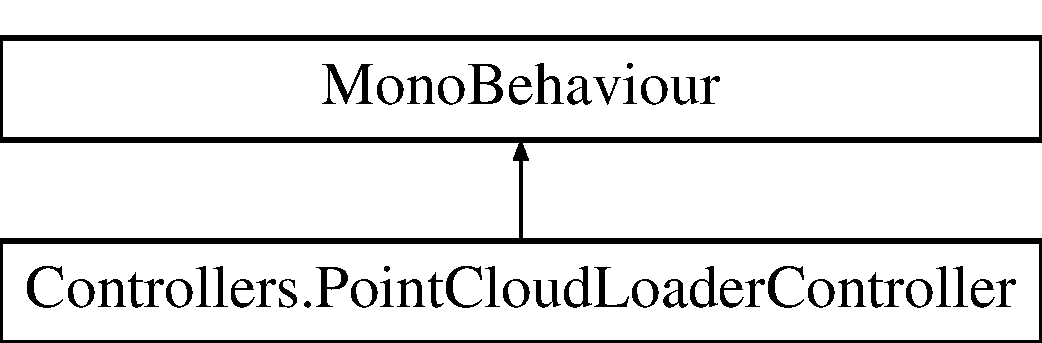
\includegraphics[height=2.000000cm]{class_controllers_1_1_point_cloud_loader_controller}
\end{center}
\end{figure}
\subsection*{Public Attributes}
\begin{DoxyCompactItemize}
\item 
\mbox{\Hypertarget{class_controllers_1_1_point_cloud_loader_controller_ab078f86da48d6f30533fc56e55afd46a}\label{class_controllers_1_1_point_cloud_loader_controller_ab078f86da48d6f30533fc56e55afd46a}} 
string {\bfseries cloud\+Path}
\item 
\mbox{\Hypertarget{class_controllers_1_1_point_cloud_loader_controller_a9bb507914cb9523f6199752ea6f94408}\label{class_controllers_1_1_point_cloud_loader_controller_a9bb507914cb9523f6199752ea6f94408}} 
\hyperlink{class_object_creation_1_1_mesh_configuration}{Mesh\+Configuration} {\bfseries mesh\+Configuration}
\item 
\mbox{\Hypertarget{class_controllers_1_1_point_cloud_loader_controller_a44e6b8b4c81612f9376d587033b4220f}\label{class_controllers_1_1_point_cloud_loader_controller_a44e6b8b4c81612f9376d587033b4220f}} 
bool {\bfseries move\+To\+Origin}
\end{DoxyCompactItemize}


The documentation for this class was generated from the following file\+:\begin{DoxyCompactItemize}
\item 
Controllers/Point\+Cloud\+Loader\+Controller.\+cs\end{DoxyCompactItemize}

\hypertarget{class_cloud_data_1_1_point_cloud_meta_data}{}\section{Cloud\+Data.\+Point\+Cloud\+Meta\+Data Class Reference}
\label{class_cloud_data_1_1_point_cloud_meta_data}\index{Cloud\+Data.\+Point\+Cloud\+Meta\+Data@{Cloud\+Data.\+Point\+Cloud\+Meta\+Data}}
\subsection*{Static Public Member Functions}
\begin{DoxyCompactItemize}
\item 
\mbox{\Hypertarget{class_cloud_data_1_1_point_cloud_meta_data_a3b43afa4f8f1dd2dc70582d011e05327}\label{class_cloud_data_1_1_point_cloud_meta_data_a3b43afa4f8f1dd2dc70582d011e05327}} 
static \hyperlink{class_cloud_data_1_1_point_cloud_meta_data}{Point\+Cloud\+Meta\+Data} {\bfseries Read\+From\+Json} (string json, bool move\+To\+Origin)
\end{DoxyCompactItemize}
\subsection*{Public Attributes}
\begin{DoxyCompactItemize}
\item 
\mbox{\Hypertarget{class_cloud_data_1_1_point_cloud_meta_data_af39846e8106b90f681faff8ca445445d}\label{class_cloud_data_1_1_point_cloud_meta_data_af39846e8106b90f681faff8ca445445d}} 
string {\bfseries version}
\item 
\mbox{\Hypertarget{class_cloud_data_1_1_point_cloud_meta_data_afeacf4f57521e3eb85436adb634649c7}\label{class_cloud_data_1_1_point_cloud_meta_data_afeacf4f57521e3eb85436adb634649c7}} 
string {\bfseries octree\+Dir}
\item 
\mbox{\Hypertarget{class_cloud_data_1_1_point_cloud_meta_data_aeadb3d09144c4c83949aab25f29cf795}\label{class_cloud_data_1_1_point_cloud_meta_data_aeadb3d09144c4c83949aab25f29cf795}} 
string {\bfseries projection}
\item 
\mbox{\Hypertarget{class_cloud_data_1_1_point_cloud_meta_data_a61452987f78f29198e3dd0e43361934f}\label{class_cloud_data_1_1_point_cloud_meta_data_a61452987f78f29198e3dd0e43361934f}} 
int {\bfseries points}
\item 
\mbox{\Hypertarget{class_cloud_data_1_1_point_cloud_meta_data_ac2cddb5b550b32f17f1e773182c30746}\label{class_cloud_data_1_1_point_cloud_meta_data_ac2cddb5b550b32f17f1e773182c30746}} 
\hyperlink{class_cloud_data_1_1_bounding_box}{Bounding\+Box} {\bfseries bounding\+Box}
\item 
\mbox{\Hypertarget{class_cloud_data_1_1_point_cloud_meta_data_ae418096ef0fa99cb2175815b6b06aa5a}\label{class_cloud_data_1_1_point_cloud_meta_data_ae418096ef0fa99cb2175815b6b06aa5a}} 
\hyperlink{class_cloud_data_1_1_bounding_box}{Bounding\+Box} {\bfseries tight\+Bounding\+Box}
\item 
\mbox{\Hypertarget{class_cloud_data_1_1_point_cloud_meta_data_a35a71dbacff0d6af6edec8ecb726b928}\label{class_cloud_data_1_1_point_cloud_meta_data_a35a71dbacff0d6af6edec8ecb726b928}} 
List$<$ string $>$ {\bfseries point\+Attributes}
\item 
\mbox{\Hypertarget{class_cloud_data_1_1_point_cloud_meta_data_a498ba71c24542bd0b1adaf7638398fb4}\label{class_cloud_data_1_1_point_cloud_meta_data_a498ba71c24542bd0b1adaf7638398fb4}} 
double {\bfseries spacing}
\item 
\mbox{\Hypertarget{class_cloud_data_1_1_point_cloud_meta_data_a91b4f77e084227c8513d9c7aa16dc4b8}\label{class_cloud_data_1_1_point_cloud_meta_data_a91b4f77e084227c8513d9c7aa16dc4b8}} 
double {\bfseries scale}
\item 
\mbox{\Hypertarget{class_cloud_data_1_1_point_cloud_meta_data_a8d61903ad4dcd1ba3911f186f05ed52a}\label{class_cloud_data_1_1_point_cloud_meta_data_a8d61903ad4dcd1ba3911f186f05ed52a}} 
int {\bfseries hierarchy\+Step\+Size}
\item 
\mbox{\Hypertarget{class_cloud_data_1_1_point_cloud_meta_data_aab3f73c48181a9dc31ec03926af2da8a}\label{class_cloud_data_1_1_point_cloud_meta_data_aab3f73c48181a9dc31ec03926af2da8a}} 
string {\bfseries cloud\+Path}
\item 
\mbox{\Hypertarget{class_cloud_data_1_1_point_cloud_meta_data_a0c5632a8cf45f3ec60dabb7f9dd65864}\label{class_cloud_data_1_1_point_cloud_meta_data_a0c5632a8cf45f3ec60dabb7f9dd65864}} 
string {\bfseries cloud\+Name}
\end{DoxyCompactItemize}


The documentation for this class was generated from the following file\+:\begin{DoxyCompactItemize}
\item 
Cloud\+Data/Point\+Cloud\+Meta\+Data.\+cs\end{DoxyCompactItemize}

\hypertarget{class_controllers_1_1_point_cloud_set_multi_time_controller}{}\section{Controllers.\+Point\+Cloud\+Set\+Multi\+Time\+Controller Class Reference}
\label{class_controllers_1_1_point_cloud_set_multi_time_controller}\index{Controllers.\+Point\+Cloud\+Set\+Multi\+Time\+Controller@{Controllers.\+Point\+Cloud\+Set\+Multi\+Time\+Controller}}
Inheritance diagram for Controllers.\+Point\+Cloud\+Set\+Multi\+Time\+Controller\+:\begin{figure}[H]
\begin{center}
\leavevmode
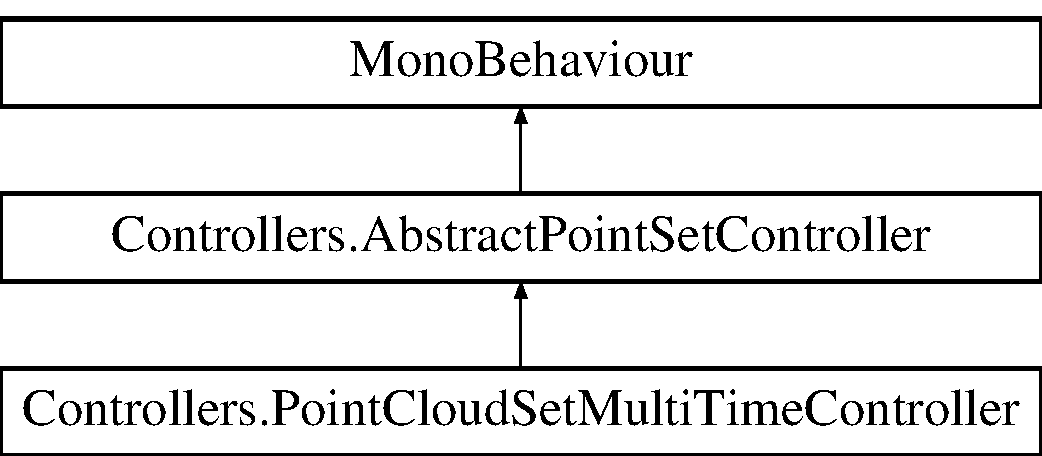
\includegraphics[height=3.000000cm]{class_controllers_1_1_point_cloud_set_multi_time_controller}
\end{center}
\end{figure}
\subsection*{Public Attributes}
\begin{DoxyCompactItemize}
\item 
\mbox{\Hypertarget{class_controllers_1_1_point_cloud_set_multi_time_controller_a645044db6bfd8f471e92324429676fc8}\label{class_controllers_1_1_point_cloud_set_multi_time_controller_a645044db6bfd8f471e92324429676fc8}} 
uint {\bfseries point\+Budget}
\item 
\mbox{\Hypertarget{class_controllers_1_1_point_cloud_set_multi_time_controller_adbd6ce51c56a5a12dd9e64263287335e}\label{class_controllers_1_1_point_cloud_set_multi_time_controller_adbd6ce51c56a5a12dd9e64263287335e}} 
int {\bfseries min\+Node\+Size}
\item 
\mbox{\Hypertarget{class_controllers_1_1_point_cloud_set_multi_time_controller_a9936cdc4a0ab3bdedc96856631d52224}\label{class_controllers_1_1_point_cloud_set_multi_time_controller_a9936cdc4a0ab3bdedc96856631d52224}} 
uint {\bfseries nodes\+Per\+Frame} = 15
\item 
\mbox{\Hypertarget{class_controllers_1_1_point_cloud_set_multi_time_controller_a6fd1ae91dff4c3735195caa4d3f7ea43}\label{class_controllers_1_1_point_cloud_set_multi_time_controller_a6fd1ae91dff4c3735195caa4d3f7ea43}} 
\hyperlink{class_object_creation_1_1_mesh_configuration}{Mesh\+Configuration} {\bfseries mesh\+Configuration}
\item 
\mbox{\Hypertarget{class_controllers_1_1_point_cloud_set_multi_time_controller_a41371a0c5548dce88c52b6005e77015f}\label{class_controllers_1_1_point_cloud_set_multi_time_controller_a41371a0c5548dce88c52b6005e77015f}} 
bool {\bfseries multithreaded} = true
\item 
\mbox{\Hypertarget{class_controllers_1_1_point_cloud_set_multi_time_controller_ab4767a6ab9bc35316f03fa94f3eca6cc}\label{class_controllers_1_1_point_cloud_set_multi_time_controller_ab4767a6ab9bc35316f03fa94f3eca6cc}} 
uint {\bfseries cache\+Size\+In\+Points} = 0
\end{DoxyCompactItemize}
\subsection*{Protected Member Functions}
\begin{DoxyCompactItemize}
\item 
\mbox{\Hypertarget{class_controllers_1_1_point_cloud_set_multi_time_controller_ada6df0cc7f76cb03cc1d2cbd948c8e9e}\label{class_controllers_1_1_point_cloud_set_multi_time_controller_ada6df0cc7f76cb03cc1d2cbd948c8e9e}} 
override void {\bfseries Initialize} ()
\end{DoxyCompactItemize}
\subsection*{Additional Inherited Members}


The documentation for this class was generated from the following file\+:\begin{DoxyCompactItemize}
\item 
Controllers/Point\+Cloud\+Set\+Multi\+Time\+Controller.\+cs\end{DoxyCompactItemize}

\hypertarget{class_controllers_1_1_point_cloud_set_one_time_controller}{}\section{Controllers.\+Point\+Cloud\+Set\+One\+Time\+Controller Class Reference}
\label{class_controllers_1_1_point_cloud_set_one_time_controller}\index{Controllers.\+Point\+Cloud\+Set\+One\+Time\+Controller@{Controllers.\+Point\+Cloud\+Set\+One\+Time\+Controller}}
Inheritance diagram for Controllers.\+Point\+Cloud\+Set\+One\+Time\+Controller\+:\begin{figure}[H]
\begin{center}
\leavevmode
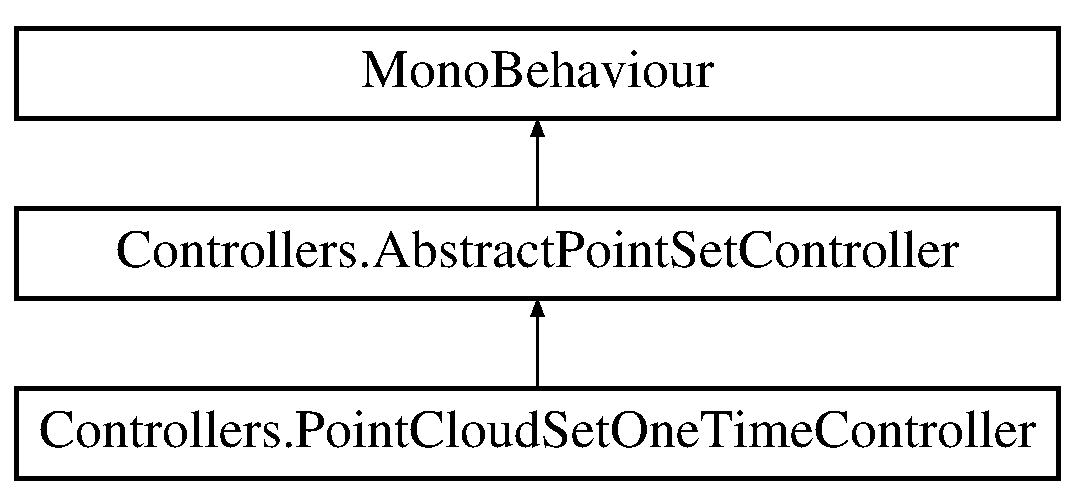
\includegraphics[height=3.000000cm]{class_controllers_1_1_point_cloud_set_one_time_controller}
\end{center}
\end{figure}
\subsection*{Public Attributes}
\begin{DoxyCompactItemize}
\item 
\mbox{\Hypertarget{class_controllers_1_1_point_cloud_set_one_time_controller_a3b44cbf21a49063a9f2d64ffe4147802}\label{class_controllers_1_1_point_cloud_set_one_time_controller_a3b44cbf21a49063a9f2d64ffe4147802}} 
uint {\bfseries point\+Budget}
\item 
\mbox{\Hypertarget{class_controllers_1_1_point_cloud_set_one_time_controller_ad7a699c80cdcd10dc56ac948205f9de4}\label{class_controllers_1_1_point_cloud_set_one_time_controller_ad7a699c80cdcd10dc56ac948205f9de4}} 
int {\bfseries min\+Node\+Size}
\item 
\mbox{\Hypertarget{class_controllers_1_1_point_cloud_set_one_time_controller_a20ba15a4209ad45a45b0ea5560a66088}\label{class_controllers_1_1_point_cloud_set_one_time_controller_a20ba15a4209ad45a45b0ea5560a66088}} 
\hyperlink{class_object_creation_1_1_mesh_configuration}{Mesh\+Configuration} {\bfseries mesh\+Configuration}
\item 
\mbox{\Hypertarget{class_controllers_1_1_point_cloud_set_one_time_controller_aaa3813d070269d1e779b4dccd4c09793}\label{class_controllers_1_1_point_cloud_set_one_time_controller_aaa3813d070269d1e779b4dccd4c09793}} 
bool {\bfseries multithreaded} = true
\end{DoxyCompactItemize}
\subsection*{Protected Member Functions}
\begin{DoxyCompactItemize}
\item 
\mbox{\Hypertarget{class_controllers_1_1_point_cloud_set_one_time_controller_a36b5907637583779902ab0ab8307c441}\label{class_controllers_1_1_point_cloud_set_one_time_controller_a36b5907637583779902ab0ab8307c441}} 
override void {\bfseries Initialize} ()
\end{DoxyCompactItemize}
\subsection*{Additional Inherited Members}


The documentation for this class was generated from the following file\+:\begin{DoxyCompactItemize}
\item 
Controllers/Point\+Cloud\+Set\+One\+Time\+Controller.\+cs\end{DoxyCompactItemize}

\hypertarget{class_controllers_1_1_point_cloud_set_real_time_controller}{}\section{Controllers.\+Point\+Cloud\+Set\+Real\+Time\+Controller Class Reference}
\label{class_controllers_1_1_point_cloud_set_real_time_controller}\index{Controllers.\+Point\+Cloud\+Set\+Real\+Time\+Controller@{Controllers.\+Point\+Cloud\+Set\+Real\+Time\+Controller}}
Inheritance diagram for Controllers.\+Point\+Cloud\+Set\+Real\+Time\+Controller\+:\begin{figure}[H]
\begin{center}
\leavevmode
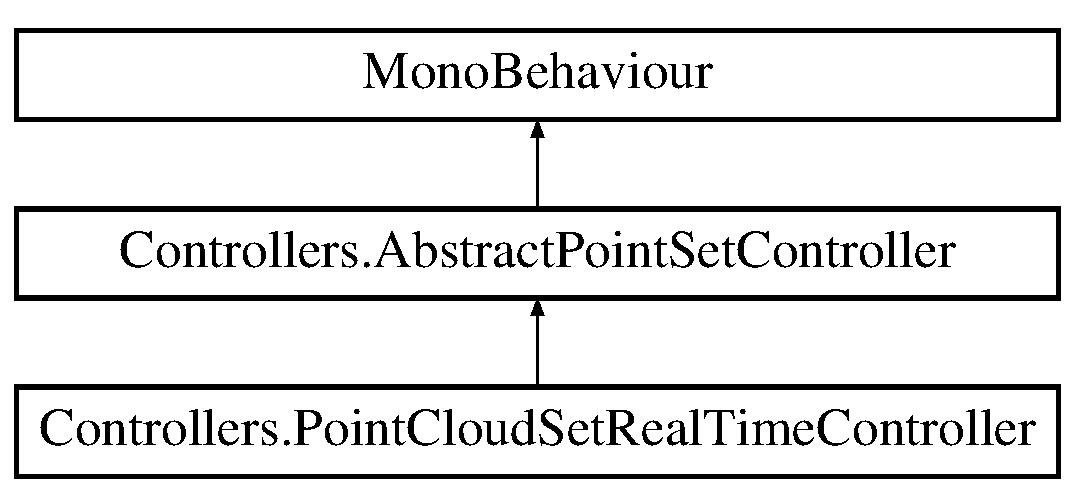
\includegraphics[height=3.000000cm]{class_controllers_1_1_point_cloud_set_real_time_controller}
\end{center}
\end{figure}
\subsection*{Public Attributes}
\begin{DoxyCompactItemize}
\item 
\mbox{\Hypertarget{class_controllers_1_1_point_cloud_set_real_time_controller_a549628d8ed3f25f10c3b76dbae85f21f}\label{class_controllers_1_1_point_cloud_set_real_time_controller_a549628d8ed3f25f10c3b76dbae85f21f}} 
uint {\bfseries point\+Budget}
\item 
\mbox{\Hypertarget{class_controllers_1_1_point_cloud_set_real_time_controller_a9f1a28c90565a0fc6682d696fb9a69f8}\label{class_controllers_1_1_point_cloud_set_real_time_controller_a9f1a28c90565a0fc6682d696fb9a69f8}} 
int {\bfseries min\+Node\+Size}
\item 
\mbox{\Hypertarget{class_controllers_1_1_point_cloud_set_real_time_controller_adc4813fd0699df3a3f346cf1f7b5fed5}\label{class_controllers_1_1_point_cloud_set_real_time_controller_adc4813fd0699df3a3f346cf1f7b5fed5}} 
uint {\bfseries nodes\+Per\+Frame} = 15
\item 
\mbox{\Hypertarget{class_controllers_1_1_point_cloud_set_real_time_controller_a8f86af88e750db2c7fea237ce00eaa5d}\label{class_controllers_1_1_point_cloud_set_real_time_controller_a8f86af88e750db2c7fea237ce00eaa5d}} 
\hyperlink{class_object_creation_1_1_mesh_configuration}{Mesh\+Configuration} {\bfseries mesh\+Configuration}
\item 
\mbox{\Hypertarget{class_controllers_1_1_point_cloud_set_real_time_controller_aa38ef6c83b9ceb3ea8389164c5c05e77}\label{class_controllers_1_1_point_cloud_set_real_time_controller_aa38ef6c83b9ceb3ea8389164c5c05e77}} 
bool {\bfseries multithreaded} = true
\item 
\mbox{\Hypertarget{class_controllers_1_1_point_cloud_set_real_time_controller_aa957e5447cd6ec2bc1c387bbb65a90ad}\label{class_controllers_1_1_point_cloud_set_real_time_controller_aa957e5447cd6ec2bc1c387bbb65a90ad}} 
uint {\bfseries cache\+Size\+In\+Points} = 0
\end{DoxyCompactItemize}
\subsection*{Protected Member Functions}
\begin{DoxyCompactItemize}
\item 
\mbox{\Hypertarget{class_controllers_1_1_point_cloud_set_real_time_controller_a201cc0a4cf300d304ee090d138fc8637}\label{class_controllers_1_1_point_cloud_set_real_time_controller_a201cc0a4cf300d304ee090d138fc8637}} 
override void {\bfseries Initialize} ()
\end{DoxyCompactItemize}
\subsection*{Additional Inherited Members}


The documentation for this class was generated from the following file\+:\begin{DoxyCompactItemize}
\item 
Controllers/Point\+Cloud\+Set\+Real\+Time\+Controller.\+cs\end{DoxyCompactItemize}

\hypertarget{class_object_creation_1_1_point_mesh_configuration}{}\section{Object\+Creation.\+Point\+Mesh\+Configuration Class Reference}
\label{class_object_creation_1_1_point_mesh_configuration}\index{Object\+Creation.\+Point\+Mesh\+Configuration@{Object\+Creation.\+Point\+Mesh\+Configuration}}
Inheritance diagram for Object\+Creation.\+Point\+Mesh\+Configuration\+:\begin{figure}[H]
\begin{center}
\leavevmode
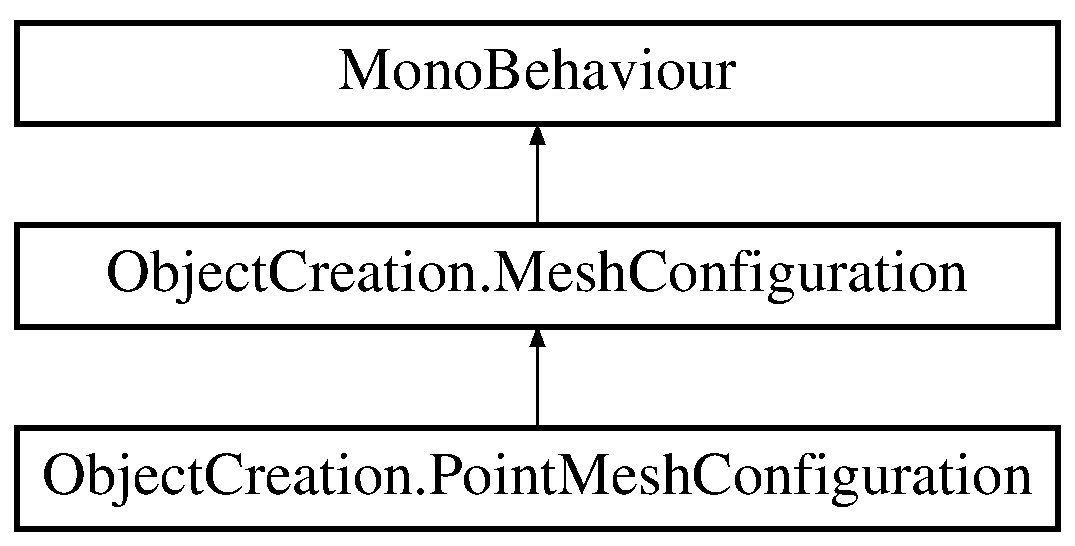
\includegraphics[height=3.000000cm]{class_object_creation_1_1_point_mesh_configuration}
\end{center}
\end{figure}
\subsection*{Public Member Functions}
\begin{DoxyCompactItemize}
\item 
\mbox{\Hypertarget{class_object_creation_1_1_point_mesh_configuration_ad910bfac398c68f9b65103df5de9f9ec}\label{class_object_creation_1_1_point_mesh_configuration_ad910bfac398c68f9b65103df5de9f9ec}} 
void {\bfseries Start} ()
\item 
\mbox{\Hypertarget{class_object_creation_1_1_point_mesh_configuration_a9bf5872344d3848dc39b9287396d4bd8}\label{class_object_creation_1_1_point_mesh_configuration_a9bf5872344d3848dc39b9287396d4bd8}} 
override Game\+Object {\bfseries Create\+Game\+Object} (string name, Vector3\mbox{[}$\,$\mbox{]} vertex\+Data, Color\mbox{[}$\,$\mbox{]} color\+Data, \hyperlink{class_cloud_data_1_1_bounding_box}{Bounding\+Box} bounding\+Box)
\item 
\mbox{\Hypertarget{class_object_creation_1_1_point_mesh_configuration_a52ff0f63947113009274de7e815f472a}\label{class_object_creation_1_1_point_mesh_configuration_a52ff0f63947113009274de7e815f472a}} 
override int {\bfseries Get\+Maximum\+Points\+Per\+Mesh} ()
\item 
\mbox{\Hypertarget{class_object_creation_1_1_point_mesh_configuration_aa8b986ffcec27061b4277605b2641aca}\label{class_object_creation_1_1_point_mesh_configuration_aa8b986ffcec27061b4277605b2641aca}} 
override void {\bfseries Remove\+Game\+Object} (Game\+Object game\+Object)
\end{DoxyCompactItemize}


The documentation for this class was generated from the following file\+:\begin{DoxyCompactItemize}
\item 
Object\+Creation/Point\+Mesh\+Configuration.\+cs\end{DoxyCompactItemize}

\hypertarget{class_data_structures_1_1_priority_queue}{}\section{Data\+Structures.\+Priority\+Queue$<$ I, T $>$ Class Template Reference}
\label{class_data_structures_1_1_priority_queue}\index{Data\+Structures.\+Priority\+Queue$<$ I, T $>$@{Data\+Structures.\+Priority\+Queue$<$ I, T $>$}}
Inheritance diagram for Data\+Structures.\+Priority\+Queue$<$ I, T $>$\+:\begin{figure}[H]
\begin{center}
\leavevmode
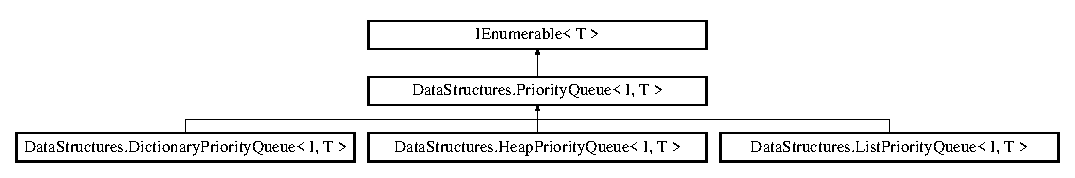
\includegraphics[height=1.944444cm]{class_data_structures_1_1_priority_queue}
\end{center}
\end{figure}
\subsection*{Public Member Functions}
\begin{DoxyCompactItemize}
\item 
\mbox{\Hypertarget{class_data_structures_1_1_priority_queue_a61be8a39a46e024b9c525e303c2e3a9c}\label{class_data_structures_1_1_priority_queue_a61be8a39a46e024b9c525e303c2e3a9c}} 
abstract void {\bfseries Enqueue} (T element, I priority)
\item 
\mbox{\Hypertarget{class_data_structures_1_1_priority_queue_a8a732750bad53930ba59e9d53893efd0}\label{class_data_structures_1_1_priority_queue_a8a732750bad53930ba59e9d53893efd0}} 
abstract T {\bfseries Dequeue} ()
\item 
\mbox{\Hypertarget{class_data_structures_1_1_priority_queue_a9e1ce2ebad51263dee248c2e2538946a}\label{class_data_structures_1_1_priority_queue_a9e1ce2ebad51263dee248c2e2538946a}} 
abstract T {\bfseries Dequeue} (out I priority)
\item 
\mbox{\Hypertarget{class_data_structures_1_1_priority_queue_ab4b2bddca269934a3f208bf0070fd392}\label{class_data_structures_1_1_priority_queue_ab4b2bddca269934a3f208bf0070fd392}} 
abstract I {\bfseries Max\+Priority} ()
\item 
\mbox{\Hypertarget{class_data_structures_1_1_priority_queue_a91777550673283c472a559a87735b7a9}\label{class_data_structures_1_1_priority_queue_a91777550673283c472a559a87735b7a9}} 
abstract T {\bfseries Peek} ()
\item 
\mbox{\Hypertarget{class_data_structures_1_1_priority_queue_abc51f812d0d3fac90e7d5b5ef9a1e245}\label{class_data_structures_1_1_priority_queue_abc51f812d0d3fac90e7d5b5ef9a1e245}} 
abstract void {\bfseries Remove} (T element, I priority)
\item 
\mbox{\Hypertarget{class_data_structures_1_1_priority_queue_a5736c78300aa3cfcb633d3676c8fb20e}\label{class_data_structures_1_1_priority_queue_a5736c78300aa3cfcb633d3676c8fb20e}} 
abstract void {\bfseries Remove} (T element)
\item 
\mbox{\Hypertarget{class_data_structures_1_1_priority_queue_a8dfb2ec9123a0c60c28098b388e1e545}\label{class_data_structures_1_1_priority_queue_a8dfb2ec9123a0c60c28098b388e1e545}} 
abstract void {\bfseries Clear} ()
\item 
\mbox{\Hypertarget{class_data_structures_1_1_priority_queue_ae632f425192bffb62ba226b3c4a09111}\label{class_data_structures_1_1_priority_queue_ae632f425192bffb62ba226b3c4a09111}} 
abstract bool {\bfseries Is\+Empty} ()
\item 
\mbox{\Hypertarget{class_data_structures_1_1_priority_queue_a91546a1854a4aa9c404b83c4f2f630b7}\label{class_data_structures_1_1_priority_queue_a91546a1854a4aa9c404b83c4f2f630b7}} 
abstract I\+Enumerator$<$ T $>$ {\bfseries Get\+Enumerator} ()
\end{DoxyCompactItemize}
\subsection*{Properties}
\begin{DoxyCompactItemize}
\item 
\mbox{\Hypertarget{class_data_structures_1_1_priority_queue_aec35247de1b30d371da5c9d3d2e01407}\label{class_data_structures_1_1_priority_queue_aec35247de1b30d371da5c9d3d2e01407}} 
abstract int {\bfseries Count}\hspace{0.3cm}{\ttfamily  \mbox{[}get\mbox{]}}
\end{DoxyCompactItemize}


The documentation for this class was generated from the following file\+:\begin{DoxyCompactItemize}
\item 
Data\+Structures/Priority\+Queue.\+cs\end{DoxyCompactItemize}

\hypertarget{class_object_creation_1_1_quad4_point_mesh_configuration}{}\section{Object\+Creation.\+Quad4\+Point\+Mesh\+Configuration Class Reference}
\label{class_object_creation_1_1_quad4_point_mesh_configuration}\index{Object\+Creation.\+Quad4\+Point\+Mesh\+Configuration@{Object\+Creation.\+Quad4\+Point\+Mesh\+Configuration}}
Inheritance diagram for Object\+Creation.\+Quad4\+Point\+Mesh\+Configuration\+:\begin{figure}[H]
\begin{center}
\leavevmode
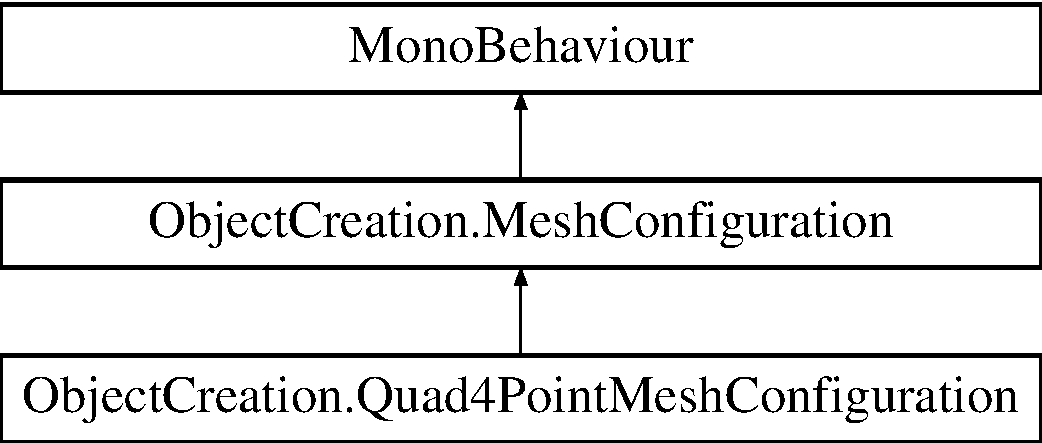
\includegraphics[height=3.000000cm]{class_object_creation_1_1_quad4_point_mesh_configuration}
\end{center}
\end{figure}
\subsection*{Public Member Functions}
\begin{DoxyCompactItemize}
\item 
\mbox{\Hypertarget{class_object_creation_1_1_quad4_point_mesh_configuration_a4dd9de3bf8bf9e370c8d6f88b95e4995}\label{class_object_creation_1_1_quad4_point_mesh_configuration_a4dd9de3bf8bf9e370c8d6f88b95e4995}} 
void {\bfseries Start} ()
\item 
\mbox{\Hypertarget{class_object_creation_1_1_quad4_point_mesh_configuration_a26c187f6c0e3ac5b718be8e0c1d7b57d}\label{class_object_creation_1_1_quad4_point_mesh_configuration_a26c187f6c0e3ac5b718be8e0c1d7b57d}} 
override Game\+Object {\bfseries Create\+Game\+Object} (string name, Vector3\mbox{[}$\,$\mbox{]} vertex\+Data, Color\mbox{[}$\,$\mbox{]} color\+Data, \hyperlink{class_cloud_data_1_1_bounding_box}{Bounding\+Box} bounding\+Box)
\item 
\mbox{\Hypertarget{class_object_creation_1_1_quad4_point_mesh_configuration_a1d54b547c414a98403352fdddef302b9}\label{class_object_creation_1_1_quad4_point_mesh_configuration_a1d54b547c414a98403352fdddef302b9}} 
override int {\bfseries Get\+Maximum\+Points\+Per\+Mesh} ()
\item 
\mbox{\Hypertarget{class_object_creation_1_1_quad4_point_mesh_configuration_a5aaef0f45da279e17151df577a7b7c87}\label{class_object_creation_1_1_quad4_point_mesh_configuration_a5aaef0f45da279e17151df577a7b7c87}} 
override void {\bfseries Remove\+Game\+Object} (Game\+Object game\+Object)
\end{DoxyCompactItemize}
\subsection*{Public Attributes}
\begin{DoxyCompactItemize}
\item 
\mbox{\Hypertarget{class_object_creation_1_1_quad4_point_mesh_configuration_ac73682bf5cf39ce2d854d5463b9ae112}\label{class_object_creation_1_1_quad4_point_mesh_configuration_ac73682bf5cf39ce2d854d5463b9ae112}} 
float {\bfseries point\+Radius} = 10
\item 
\mbox{\Hypertarget{class_object_creation_1_1_quad4_point_mesh_configuration_abb11b39a3a00e3060e2b48f19beb0d3c}\label{class_object_creation_1_1_quad4_point_mesh_configuration_abb11b39a3a00e3060e2b48f19beb0d3c}} 
bool {\bfseries render\+Circles} = false
\end{DoxyCompactItemize}


The documentation for this class was generated from the following file\+:\begin{DoxyCompactItemize}
\item 
Object\+Creation/Quad4\+Point\+Mesh\+Configuration.\+cs\end{DoxyCompactItemize}

\hypertarget{class_data_structures_1_1_random_access_queue}{}\section{Data\+Structures.\+Random\+Access\+Queue$<$ T $>$ Class Template Reference}
\label{class_data_structures_1_1_random_access_queue}\index{Data\+Structures.\+Random\+Access\+Queue$<$ T $>$@{Data\+Structures.\+Random\+Access\+Queue$<$ T $>$}}
\subsection*{Public Member Functions}
\begin{DoxyCompactItemize}
\item 
\mbox{\Hypertarget{class_data_structures_1_1_random_access_queue_a4596a5d2823e0bd998677cc66b2289ed}\label{class_data_structures_1_1_random_access_queue_a4596a5d2823e0bd998677cc66b2289ed}} 
void {\bfseries Enqueue} (T element)
\item 
\mbox{\Hypertarget{class_data_structures_1_1_random_access_queue_a40ceaaa7ccd5cb960daaf2f7ae4cdb66}\label{class_data_structures_1_1_random_access_queue_a40ceaaa7ccd5cb960daaf2f7ae4cdb66}} 
T {\bfseries Dequeue} ()
\item 
\mbox{\Hypertarget{class_data_structures_1_1_random_access_queue_a754cec5b81c1339d5050d89377a249a4}\label{class_data_structures_1_1_random_access_queue_a754cec5b81c1339d5050d89377a249a4}} 
bool {\bfseries Is\+Empty} ()
\item 
\mbox{\Hypertarget{class_data_structures_1_1_random_access_queue_aea5da6dc093d903a3ed488a32147135e}\label{class_data_structures_1_1_random_access_queue_aea5da6dc093d903a3ed488a32147135e}} 
void {\bfseries Clear} ()
\item 
\mbox{\Hypertarget{class_data_structures_1_1_random_access_queue_a8abf10e6b7f7c3cf7d8f50087c8f7b7f}\label{class_data_structures_1_1_random_access_queue_a8abf10e6b7f7c3cf7d8f50087c8f7b7f}} 
void {\bfseries Remove} (T element)
\item 
\mbox{\Hypertarget{class_data_structures_1_1_random_access_queue_a25e36b80c04362e1e803e529165b7706}\label{class_data_structures_1_1_random_access_queue_a25e36b80c04362e1e803e529165b7706}} 
bool {\bfseries Contains} (T element)
\end{DoxyCompactItemize}


The documentation for this class was generated from the following file\+:\begin{DoxyCompactItemize}
\item 
Data\+Structures/Random\+Access\+Queue.\+cs\end{DoxyCompactItemize}

\hypertarget{class_loading_1_1_single_threaded_multi_time_renderer}{}\section{Loading.\+Single\+Threaded\+Multi\+Time\+Renderer Class Reference}
\label{class_loading_1_1_single_threaded_multi_time_renderer}\index{Loading.\+Single\+Threaded\+Multi\+Time\+Renderer@{Loading.\+Single\+Threaded\+Multi\+Time\+Renderer}}
Inheritance diagram for Loading.\+Single\+Threaded\+Multi\+Time\+Renderer\+:\begin{figure}[H]
\begin{center}
\leavevmode
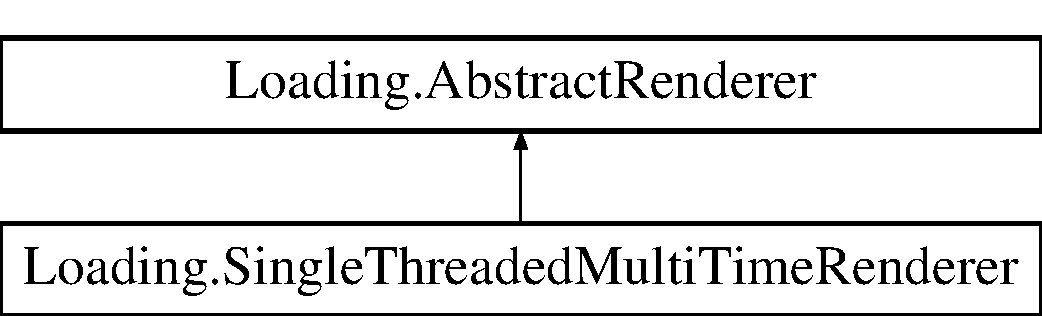
\includegraphics[height=2.000000cm]{class_loading_1_1_single_threaded_multi_time_renderer}
\end{center}
\end{figure}
\subsection*{Public Member Functions}
\begin{DoxyCompactItemize}
\item 
\mbox{\Hypertarget{class_loading_1_1_single_threaded_multi_time_renderer_a649c7e2dade5367b325247c8e52dd6cb}\label{class_loading_1_1_single_threaded_multi_time_renderer_a649c7e2dade5367b325247c8e52dd6cb}} 
{\bfseries Single\+Threaded\+Multi\+Time\+Renderer} (int min\+Node\+Size, uint point\+Budget, uint nodes\+Per\+Frame, Camera camera, \hyperlink{class_object_creation_1_1_mesh_configuration}{Mesh\+Configuration} config)
\item 
\mbox{\Hypertarget{class_loading_1_1_single_threaded_multi_time_renderer_acac293127e86bf366b8f6f1fcf0fcb8d}\label{class_loading_1_1_single_threaded_multi_time_renderer_acac293127e86bf366b8f6f1fcf0fcb8d}} 
void {\bfseries Add\+Root\+Node} (\hyperlink{class_cloud_data_1_1_node}{Node} root\+Node)
\item 
\mbox{\Hypertarget{class_loading_1_1_single_threaded_multi_time_renderer_aac03e886194621b06aee2661a556e199}\label{class_loading_1_1_single_threaded_multi_time_renderer_aac03e886194621b06aee2661a556e199}} 
int {\bfseries Get\+Root\+Node\+Count} ()
\item 
\mbox{\Hypertarget{class_loading_1_1_single_threaded_multi_time_renderer_a388989b16b51b2facbbd9384ebf42bdd}\label{class_loading_1_1_single_threaded_multi_time_renderer_a388989b16b51b2facbbd9384ebf42bdd}} 
bool {\bfseries Is\+Ready\+For\+Update} ()
\item 
\mbox{\Hypertarget{class_loading_1_1_single_threaded_multi_time_renderer_aa9085a1fcd401178f9ad7f091c636c52}\label{class_loading_1_1_single_threaded_multi_time_renderer_aa9085a1fcd401178f9ad7f091c636c52}} 
void {\bfseries Update\+Visible\+Nodes} ()
\item 
\mbox{\Hypertarget{class_loading_1_1_single_threaded_multi_time_renderer_a67525443650af03f6d9a992ca6268e9c}\label{class_loading_1_1_single_threaded_multi_time_renderer_a67525443650af03f6d9a992ca6268e9c}} 
void {\bfseries Update\+Game\+Objects} ()
\item 
\mbox{\Hypertarget{class_loading_1_1_single_threaded_multi_time_renderer_a4ae66f4ef13754c92fb3313e8eb60cb6}\label{class_loading_1_1_single_threaded_multi_time_renderer_a4ae66f4ef13754c92fb3313e8eb60cb6}} 
void {\bfseries Shut\+Down} ()
\item 
\mbox{\Hypertarget{class_loading_1_1_single_threaded_multi_time_renderer_aa2a4d051b7d089ae7d57ca19a0e157e0}\label{class_loading_1_1_single_threaded_multi_time_renderer_aa2a4d051b7d089ae7d57ca19a0e157e0}} 
uint {\bfseries Get\+Point\+Count} ()
\end{DoxyCompactItemize}


The documentation for this class was generated from the following file\+:\begin{DoxyCompactItemize}
\item 
Loading/Single\+Threaded\+Multi\+Time\+Renderer.\+cs\end{DoxyCompactItemize}

\hypertarget{class_loading_1_1_single_threaded_one_time_renderer}{}\section{Loading.\+Single\+Threaded\+One\+Time\+Renderer Class Reference}
\label{class_loading_1_1_single_threaded_one_time_renderer}\index{Loading.\+Single\+Threaded\+One\+Time\+Renderer@{Loading.\+Single\+Threaded\+One\+Time\+Renderer}}
Inheritance diagram for Loading.\+Single\+Threaded\+One\+Time\+Renderer\+:\begin{figure}[H]
\begin{center}
\leavevmode
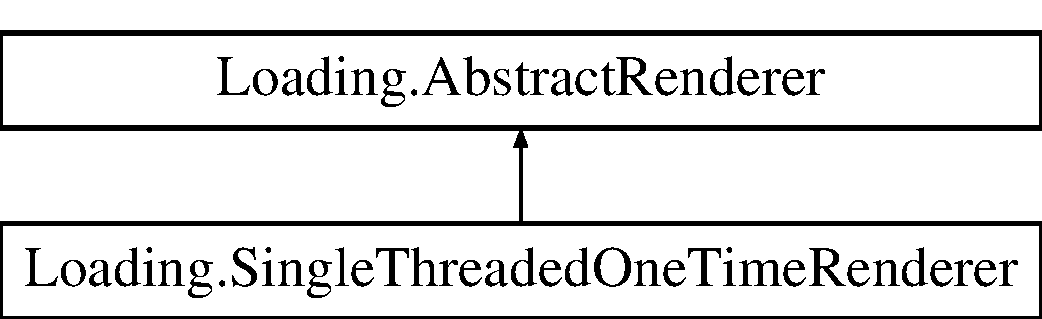
\includegraphics[height=2.000000cm]{class_loading_1_1_single_threaded_one_time_renderer}
\end{center}
\end{figure}
\subsection*{Public Member Functions}
\begin{DoxyCompactItemize}
\item 
\mbox{\Hypertarget{class_loading_1_1_single_threaded_one_time_renderer_a7f261d91f4a021ab8318a7f63b8fc990}\label{class_loading_1_1_single_threaded_one_time_renderer_a7f261d91f4a021ab8318a7f63b8fc990}} 
{\bfseries Single\+Threaded\+One\+Time\+Renderer} (int min\+Node\+Size, uint point\+Budget, Camera camera, \hyperlink{class_object_creation_1_1_mesh_configuration}{Mesh\+Configuration} config)
\item 
\mbox{\Hypertarget{class_loading_1_1_single_threaded_one_time_renderer_a7d3bdf0ddaa09b3e87191038ee4fd483}\label{class_loading_1_1_single_threaded_one_time_renderer_a7d3bdf0ddaa09b3e87191038ee4fd483}} 
void {\bfseries Add\+Root\+Node} (\hyperlink{class_cloud_data_1_1_node}{Node} root\+Node)
\item 
\mbox{\Hypertarget{class_loading_1_1_single_threaded_one_time_renderer_a89b7b8dd02941271027437efba286ea7}\label{class_loading_1_1_single_threaded_one_time_renderer_a89b7b8dd02941271027437efba286ea7}} 
int {\bfseries Get\+Root\+Node\+Count} ()
\item 
\mbox{\Hypertarget{class_loading_1_1_single_threaded_one_time_renderer_acd280bc98ac2c866c891e369a6eb6d2a}\label{class_loading_1_1_single_threaded_one_time_renderer_acd280bc98ac2c866c891e369a6eb6d2a}} 
bool {\bfseries Is\+Ready\+For\+Update} ()
\item 
\mbox{\Hypertarget{class_loading_1_1_single_threaded_one_time_renderer_a6d53bd4a48e64c8755fa2fc394aa17ec}\label{class_loading_1_1_single_threaded_one_time_renderer_a6d53bd4a48e64c8755fa2fc394aa17ec}} 
void {\bfseries Update\+Visible\+Nodes} ()
\item 
\mbox{\Hypertarget{class_loading_1_1_single_threaded_one_time_renderer_a119ad5491373db0ade423c6bd1c05322}\label{class_loading_1_1_single_threaded_one_time_renderer_a119ad5491373db0ade423c6bd1c05322}} 
void {\bfseries Update\+Game\+Objects} ()
\item 
\mbox{\Hypertarget{class_loading_1_1_single_threaded_one_time_renderer_a94efd87eec7c2b0e94a8792d6dcbee8c}\label{class_loading_1_1_single_threaded_one_time_renderer_a94efd87eec7c2b0e94a8792d6dcbee8c}} 
void {\bfseries Shut\+Down} ()
\item 
\mbox{\Hypertarget{class_loading_1_1_single_threaded_one_time_renderer_a653406032c57fa5a6bdc759c36694de9}\label{class_loading_1_1_single_threaded_one_time_renderer_a653406032c57fa5a6bdc759c36694de9}} 
uint {\bfseries Get\+Point\+Count} ()
\end{DoxyCompactItemize}


The documentation for this class was generated from the following file\+:\begin{DoxyCompactItemize}
\item 
Loading/Single\+Threaded\+One\+Time\+Renderer.\+cs\end{DoxyCompactItemize}

\hypertarget{class_data_structures_1_1_thread_safe_hash_set}{}\section{Data\+Structures.\+Thread\+Safe\+Hash\+Set$<$ T $>$ Class Template Reference}
\label{class_data_structures_1_1_thread_safe_hash_set}\index{Data\+Structures.\+Thread\+Safe\+Hash\+Set$<$ T $>$@{Data\+Structures.\+Thread\+Safe\+Hash\+Set$<$ T $>$}}
\subsection*{Public Member Functions}
\begin{DoxyCompactItemize}
\item 
\mbox{\Hypertarget{class_data_structures_1_1_thread_safe_hash_set_a94dea60b9b381fd3c1ec832101fde30e}\label{class_data_structures_1_1_thread_safe_hash_set_a94dea60b9b381fd3c1ec832101fde30e}} 
void {\bfseries Add} (T element)
\item 
\mbox{\Hypertarget{class_data_structures_1_1_thread_safe_hash_set_ae1b471930fe170dd74c91ea00f6768c0}\label{class_data_structures_1_1_thread_safe_hash_set_ae1b471930fe170dd74c91ea00f6768c0}} 
bool {\bfseries Contains} (T element)
\item 
\mbox{\Hypertarget{class_data_structures_1_1_thread_safe_hash_set_a746ae0938ea3ba645fae665db71ec5e9}\label{class_data_structures_1_1_thread_safe_hash_set_a746ae0938ea3ba645fae665db71ec5e9}} 
void {\bfseries Clear} ()
\item 
\mbox{\Hypertarget{class_data_structures_1_1_thread_safe_hash_set_a283fab4177808d5d12d2963eb1fe2cf5}\label{class_data_structures_1_1_thread_safe_hash_set_a283fab4177808d5d12d2963eb1fe2cf5}} 
void {\bfseries Remove} (T element)
\end{DoxyCompactItemize}


The documentation for this class was generated from the following file\+:\begin{DoxyCompactItemize}
\item 
Data\+Structures/Thread\+Safe\+Hash\+Set.\+cs\end{DoxyCompactItemize}

\hypertarget{class_data_structures_1_1_thread_safe_queue}{}\section{Data\+Structures.\+Thread\+Safe\+Queue$<$ T $>$ Class Template Reference}
\label{class_data_structures_1_1_thread_safe_queue}\index{Data\+Structures.\+Thread\+Safe\+Queue$<$ T $>$@{Data\+Structures.\+Thread\+Safe\+Queue$<$ T $>$}}
Inheritance diagram for Data\+Structures.\+Thread\+Safe\+Queue$<$ T $>$\+:\begin{figure}[H]
\begin{center}
\leavevmode
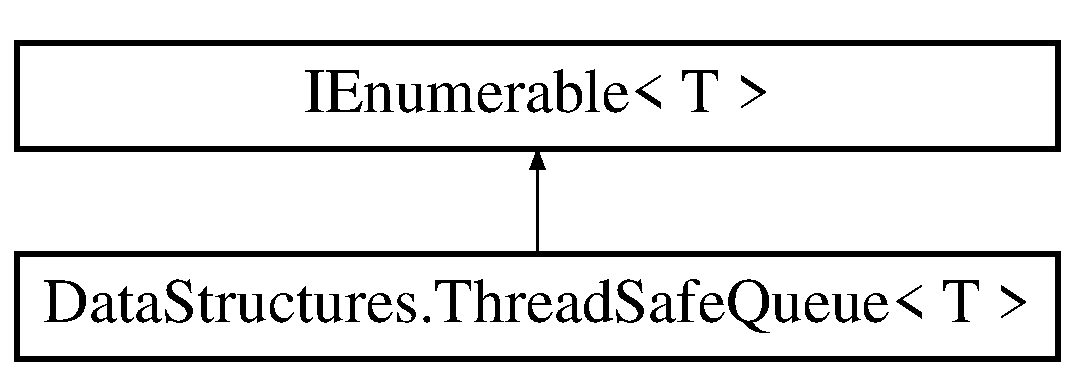
\includegraphics[height=2.000000cm]{class_data_structures_1_1_thread_safe_queue}
\end{center}
\end{figure}
\subsection*{Public Member Functions}
\begin{DoxyCompactItemize}
\item 
\mbox{\Hypertarget{class_data_structures_1_1_thread_safe_queue_a57eb48417bd3dbf530d1497836d8d41c}\label{class_data_structures_1_1_thread_safe_queue_a57eb48417bd3dbf530d1497836d8d41c}} 
void {\bfseries Enqueue} (T element)
\item 
\mbox{\Hypertarget{class_data_structures_1_1_thread_safe_queue_add3e3c658a7ce2fc165f257a7e9a36fb}\label{class_data_structures_1_1_thread_safe_queue_add3e3c658a7ce2fc165f257a7e9a36fb}} 
T {\bfseries Dequeue} ()
\item 
\mbox{\Hypertarget{class_data_structures_1_1_thread_safe_queue_a86d845c86dc2bb0aeed5ed76409dbe36}\label{class_data_structures_1_1_thread_safe_queue_a86d845c86dc2bb0aeed5ed76409dbe36}} 
bool {\bfseries Is\+Empty} ()
\item 
\mbox{\Hypertarget{class_data_structures_1_1_thread_safe_queue_a201ea8199e7fad098a862a26c19f4358}\label{class_data_structures_1_1_thread_safe_queue_a201ea8199e7fad098a862a26c19f4358}} 
void {\bfseries Clear} ()
\item 
\mbox{\Hypertarget{class_data_structures_1_1_thread_safe_queue_ad81782d74263c1758cab54c148800c48}\label{class_data_structures_1_1_thread_safe_queue_ad81782d74263c1758cab54c148800c48}} 
I\+Enumerator$<$ T $>$ {\bfseries Get\+Enumerator} ()
\end{DoxyCompactItemize}
\subsection*{Properties}
\begin{DoxyCompactItemize}
\item 
\mbox{\Hypertarget{class_data_structures_1_1_thread_safe_queue_af36d256d73d824356ad93c686d7c5aff}\label{class_data_structures_1_1_thread_safe_queue_af36d256d73d824356ad93c686d7c5aff}} 
int {\bfseries Count}\hspace{0.3cm}{\ttfamily  \mbox{[}get\mbox{]}}
\end{DoxyCompactItemize}


The documentation for this class was generated from the following file\+:\begin{DoxyCompactItemize}
\item 
Data\+Structures/Thread\+Safe\+Queue.\+cs\end{DoxyCompactItemize}

\hypertarget{class_cloud_data_1_1_vector3d}{}\section{Cloud\+Data.\+Vector3d Class Reference}
\label{class_cloud_data_1_1_vector3d}\index{Cloud\+Data.\+Vector3d@{Cloud\+Data.\+Vector3d}}
\subsection*{Public Member Functions}
\begin{DoxyCompactItemize}
\item 
\mbox{\Hypertarget{class_cloud_data_1_1_vector3d_ad2881cceccb024d4ef4199bfc929fcf8}\label{class_cloud_data_1_1_vector3d_ad2881cceccb024d4ef4199bfc929fcf8}} 
{\bfseries Vector3d} (double x, double y, double z)
\item 
\mbox{\Hypertarget{class_cloud_data_1_1_vector3d_a088e6cdaef20806391cdc35efd2e391c}\label{class_cloud_data_1_1_vector3d_a088e6cdaef20806391cdc35efd2e391c}} 
{\bfseries Vector3d} (Vector3 original)
\item 
\mbox{\Hypertarget{class_cloud_data_1_1_vector3d_aceee287d1095923c8e2daf3bb9065ef8}\label{class_cloud_data_1_1_vector3d_aceee287d1095923c8e2daf3bb9065ef8}} 
double {\bfseries Length} ()
\item 
\mbox{\Hypertarget{class_cloud_data_1_1_vector3d_a5a8514c9c89cfae9e22e4ee5835b0e8f}\label{class_cloud_data_1_1_vector3d_a5a8514c9c89cfae9e22e4ee5835b0e8f}} 
Vector3 {\bfseries To\+Float\+Vector} ()
\item 
\mbox{\Hypertarget{class_cloud_data_1_1_vector3d_ab9c83d4bca9b0f61d30536eb897abf52}\label{class_cloud_data_1_1_vector3d_ab9c83d4bca9b0f61d30536eb897abf52}} 
double {\bfseries Distance} (\hyperlink{class_cloud_data_1_1_vector3d}{Vector3d} other)
\item 
\mbox{\Hypertarget{class_cloud_data_1_1_vector3d_a4c52053302fdfe5c09a69397b80df797}\label{class_cloud_data_1_1_vector3d_a4c52053302fdfe5c09a69397b80df797}} 
\hyperlink{class_cloud_data_1_1_vector3d}{Vector3d} {\bfseries Normalize} ()
\item 
\mbox{\Hypertarget{class_cloud_data_1_1_vector3d_affd049ff0e11d92fffbc0627f31e281f}\label{class_cloud_data_1_1_vector3d_affd049ff0e11d92fffbc0627f31e281f}} 
override string {\bfseries To\+String} ()
\end{DoxyCompactItemize}
\subsection*{Static Public Member Functions}
\begin{DoxyCompactItemize}
\item 
\mbox{\Hypertarget{class_cloud_data_1_1_vector3d_aceaf280765581c7b4f6640fde768c358}\label{class_cloud_data_1_1_vector3d_aceaf280765581c7b4f6640fde768c358}} 
static \hyperlink{class_cloud_data_1_1_vector3d}{Vector3d} {\bfseries operator/} (\hyperlink{class_cloud_data_1_1_vector3d}{Vector3d} v, double divisor)
\item 
\mbox{\Hypertarget{class_cloud_data_1_1_vector3d_aa43cbef9652a38103a8a2e69160fe1bd}\label{class_cloud_data_1_1_vector3d_aa43cbef9652a38103a8a2e69160fe1bd}} 
static \hyperlink{class_cloud_data_1_1_vector3d}{Vector3d} {\bfseries operator+} (\hyperlink{class_cloud_data_1_1_vector3d}{Vector3d} a, \hyperlink{class_cloud_data_1_1_vector3d}{Vector3d} b)
\item 
\mbox{\Hypertarget{class_cloud_data_1_1_vector3d_a0ee87d5fd376a06e4b773608b7e77398}\label{class_cloud_data_1_1_vector3d_a0ee87d5fd376a06e4b773608b7e77398}} 
static \hyperlink{class_cloud_data_1_1_vector3d}{Vector3d} {\bfseries operator-\/} (\hyperlink{class_cloud_data_1_1_vector3d}{Vector3d} a, \hyperlink{class_cloud_data_1_1_vector3d}{Vector3d} b)
\item 
\mbox{\Hypertarget{class_cloud_data_1_1_vector3d_a211814063abd268494242f20e8d3672e}\label{class_cloud_data_1_1_vector3d_a211814063abd268494242f20e8d3672e}} 
static double {\bfseries operator$\ast$} (\hyperlink{class_cloud_data_1_1_vector3d}{Vector3d} a, \hyperlink{class_cloud_data_1_1_vector3d}{Vector3d} b)
\end{DoxyCompactItemize}
\subsection*{Public Attributes}
\begin{DoxyCompactItemize}
\item 
\mbox{\Hypertarget{class_cloud_data_1_1_vector3d_a40246eb4468163107d2d8502e6cc9dce}\label{class_cloud_data_1_1_vector3d_a40246eb4468163107d2d8502e6cc9dce}} 
double {\bfseries x}
\end{DoxyCompactItemize}


The documentation for this class was generated from the following file\+:\begin{DoxyCompactItemize}
\item 
Cloud\+Data/Vector3d.\+cs\end{DoxyCompactItemize}

%--- End generated contents ---

% Index
\backmatter
\newpage
\phantomsection
\clearemptydoublepage
\addcontentsline{toc}{chapter}{Index}
\printindex

\end{document}
